\documentclass[twoside]{book}

% Packages required by doxygen
\usepackage{fixltx2e}
\usepackage{calc}
\usepackage{doxygen}
\usepackage[export]{adjustbox} % also loads graphicx
\usepackage{graphicx}
\usepackage[utf8]{inputenc}
\usepackage{makeidx}
\usepackage{multicol}
\usepackage{multirow}
\PassOptionsToPackage{warn}{textcomp}
\usepackage{textcomp}
\usepackage[nointegrals]{wasysym}
\usepackage[table]{xcolor}

% Font selection
\usepackage[T1]{fontenc}
\usepackage[scaled=.90]{helvet}
\usepackage{courier}
\usepackage{amssymb}
\usepackage{sectsty}
\renewcommand{\familydefault}{\sfdefault}
\allsectionsfont{%
  \fontseries{bc}\selectfont%
  \color{darkgray}%
}
\renewcommand{\DoxyLabelFont}{%
  \fontseries{bc}\selectfont%
  \color{darkgray}%
}
\newcommand{\+}{\discretionary{\mbox{\scriptsize$\hookleftarrow$}}{}{}}

% Page & text layout
\usepackage{geometry}
\geometry{%
  a4paper,%
  top=2.5cm,%
  bottom=2.5cm,%
  left=2.5cm,%
  right=2.5cm%
}
\tolerance=750
\hfuzz=15pt
\hbadness=750
\setlength{\emergencystretch}{15pt}
\setlength{\parindent}{0cm}
\setlength{\parskip}{3ex plus 2ex minus 2ex}
\makeatletter
\renewcommand{\paragraph}{%
  \@startsection{paragraph}{4}{0ex}{-1.0ex}{1.0ex}{%
    \normalfont\normalsize\bfseries\SS@parafont%
  }%
}
\renewcommand{\subparagraph}{%
  \@startsection{subparagraph}{5}{0ex}{-1.0ex}{1.0ex}{%
    \normalfont\normalsize\bfseries\SS@subparafont%
  }%
}
\makeatother

% Headers & footers
\usepackage{fancyhdr}
\pagestyle{fancyplain}
\fancyhead[LE]{\fancyplain{}{\bfseries\thepage}}
\fancyhead[CE]{\fancyplain{}{}}
\fancyhead[RE]{\fancyplain{}{\bfseries\leftmark}}
\fancyhead[LO]{\fancyplain{}{\bfseries\rightmark}}
\fancyhead[CO]{\fancyplain{}{}}
\fancyhead[RO]{\fancyplain{}{\bfseries\thepage}}
\fancyfoot[LE]{\fancyplain{}{}}
\fancyfoot[CE]{\fancyplain{}{}}
\fancyfoot[RE]{\fancyplain{}{\bfseries\scriptsize Generated by Doxygen }}
\fancyfoot[LO]{\fancyplain{}{\bfseries\scriptsize Generated by Doxygen }}
\fancyfoot[CO]{\fancyplain{}{}}
\fancyfoot[RO]{\fancyplain{}{}}
\renewcommand{\footrulewidth}{0.4pt}
\renewcommand{\chaptermark}[1]{%
  \markboth{#1}{}%
}
\renewcommand{\sectionmark}[1]{%
  \markright{\thesection\ #1}%
}

% Indices & bibliography
\usepackage{natbib}
\usepackage[titles]{tocloft}
\setcounter{tocdepth}{3}
\setcounter{secnumdepth}{5}
\makeindex

% Hyperlinks (required, but should be loaded last)
\usepackage{ifpdf}
\ifpdf
  \usepackage[pdftex,pagebackref=true]{hyperref}
\else
  \usepackage[ps2pdf,pagebackref=true]{hyperref}
\fi
\hypersetup{%
  colorlinks=true,%
  linkcolor=blue,%
  citecolor=blue,%
  unicode%
}

% Custom commands
\newcommand{\clearemptydoublepage}{%
  \newpage{\pagestyle{empty}\cleardoublepage}%
}

\usepackage{caption}
\captionsetup{labelsep=space,justification=centering,font={bf},singlelinecheck=off,skip=4pt,position=top}

%===== C O N T E N T S =====

\begin{document}

% Titlepage & ToC
\hypersetup{pageanchor=false,
             bookmarksnumbered=true,
             pdfencoding=unicode
            }
\pagenumbering{roman}
\begin{titlepage}
\vspace*{7cm}
\begin{center}%
{\Large Wolk\+Connect-\/\+Cpp }\\
\vspace*{1cm}
{\large Generated by Doxygen 1.8.11}\\
\end{center}
\end{titlepage}
\clearemptydoublepage
\tableofcontents
\clearemptydoublepage
\pagenumbering{arabic}
\hypersetup{pageanchor=true}

%--- Begin generated contents ---
\chapter{Wolk\+Connect library}
\label{index}\hypertarget{index}{}Wolk\+Connect libraries are used to enable a device’s communication with \href{https://demo.wolkabout.com/#/login}{\tt Wolk\+About IoT Platform}. Using Wolk\+Connect libraries in the software or firmware of a device will drastically decrease the time to market for developers or anyone wanting to integrate their own product with Wolk\+About IoT Platform.

Wolk\+Connect libraries are intended to be used on IP enabled devices. The available Wolk\+Connect libraries (implemented in the following programming languages \href{https://github.com/Wolkabout/WolkConnect-C}{\tt C}, \href{https://github.com/Wolkabout/WolkConnect-Cpp}{\tt C++}, \href{https://github.com/Wolkabout/WolkConnect-Java-}{\tt Java}, \href{https://github.com/Wolkabout/WolkConnect-Python}{\tt Python}) are platform independent for OS based devices, with a special note that the Wolk\+Connect-\/C library is suitable to be adapted for the use on non-\/\+OS devices as Wolk\+Connect libraries have a small memory footprint.

Features of Wolk\+About IoT Platform that have been incorporated into Wolk\+Connect libraries will be disambiguated with information on how to perform these features on devices by using Wolk\+Connect’s A\+PI.

Wolk\+Connect libraries are open-\/source and released under the \href{https://github.com/Wolkabout/WolkConnect-C/blob/master/LICENSE}{\tt Apache Licence 2.\+0}. 

 \section*{Conception}





Wolk\+Connect library is intended to be used as a dependency in other firmwares or softwares that have their own existing business logic. Wolk\+Connect library is not, by any means, a single service to control the device, it is a library intended to handle all the specific communication with Wolk\+About IoT Platform.

Using Wolk\+Connect library requires minimal knowledge of Wolk\+About IoT Platform, no knowledge of the internal mechanisms and protocols of Wolk\+About IoT Platform is necessary. The user only utilises A\+P\+Is provided by Wolk\+Connect library in the User Application Layer, thereby reducing time-\/to-\/market required.

The architecture of software/firmware where Wolk\+Connect library is meant to be used is presented in {\itshape Fig.\+1.\+1}. The gray section in {\itshape Fig.\+1.\+1} represents the developer\textquotesingle{}s software/firmware.

\begin{center} \end{center} 

The gray section between the User Application Layer and the Hardware Abstraction Layer re\+Device Data\+Device Datapresents the user’s libraries and drivers that are required for his project. Providing Wolk\+Connect library with IP connectivity from the Hardware Abstraction Layer is expected from the user.

Wolk\+Connect library is separated into layers as shown in {\itshape Fig.\+1.\+2} \begin{center} \end{center} 

Wolk\+Connect libraries use IP connectivity provided by the OS, but on devices, where this not available, it is user’s responsibility to provide implementations for opening a socket and send/receive methods to the socket.

Communication between Wolk\+Connect library and Wolk\+About IoT Platform is achieved through the use of the \href{http://mqtt.org/}{\tt M\+Q\+TT messaging protocol}. Wolk\+Connect libraries have a common dependency, an implementation of an M\+Q\+TT client that will exchange data with an M\+Q\+TT server that is part of Wolk\+About IoT Platform. The communication between Wolk\+Connect library and Wolk\+About IoT Platform is made secure with the use of Secure Sockets Layer (S\+SL).

Another common dependency for Wolk\+Connect libraries is J\+S\+ON library that is used for parsing data that is exchanged with Wolk\+About IoT Platform. This data is formatted using a custom J\+S\+ON based protocol defined by Wolk\+About IoT Platform.

The high-\/level A\+PI represents what is available to the developer that is using Wolk\+Connect library. A\+P\+Is follow the naming convention of the programming language they were written in. Consult a specific Wolk\+Connect library’s documentation for more information. The A\+PI is divided into two parts\+: data management and device management. Device data is independent of device management on Wolk\+About IoT Platform and therefore has a separe A\+PI. Device management is responsible for device health and this, in turn, increases the device’s lifespan.

The A\+PI has the following functionalities that will be explained in the remainder of this document\+:
\begin{DoxyItemize}
\item \href{#connect-and-disconnect}{\tt Connect \& Disconnect}
\item \href{#sensor-readings}{\tt Sensor readings}
\item \href{#alarms}{\tt Alarm states}
\item \href{#actuators}{\tt Actuators}
\item \href{#keep-alive-mechanism}{\tt Keep alive mechanism}
\item \href{#configuration}{\tt Configuration}
\item \href{#dfu}{\tt Device Software/\+Firmware Update}
\end{DoxyItemize}



 \section*{A\+PI\textquotesingle{}s functional description}



 Wolk\+Connect libraries separate device’s functionality through the A\+PI into two distinct parts\+:


\begin{DoxyItemize}
\item {\bfseries Device data} -\/ valuable data to be exchanged with Wolk\+About IoT Platform
\item {\bfseries Device management} -\/ allows monitoring and controlling the connected device in order to maintain data delivery integrity.
\end{DoxyItemize}





\label{_connect-and-disconnect}%
 \begin{quote}
{\bfseries Connect and disconnect} \end{quote}
Every connection from Wolk\+Connect library to Wolk\+About IoT Platform is authenticated with a device key and a device password. These credentials are created on Wolk\+About IoT Platform when a device is created and are unique to that device. Only one active connection is allowed per device.

Attempting to create an additional connection with the same device credentials will terminate the previous connection. The connection is made secure, by default, in all Wolk\+Connect libraries through the use of Secure Sockets Layer (S\+SL). Connecting without S\+SL is possible. For more information, refer to specific Wolk\+Connect library documentation.

A device can be connected to Wolk\+About IoT Platform in two ways\+:


\begin{DoxyItemize}
\item {\bfseries Always connected devices} -\/ connect once and publish data when necessary. Actuations can only be used in this case, as sending actuations from Wolk\+About IoT Platform are disabled when the device is offline.
\item {\bfseries Periodically connected devices} -\/ connect and publish data when needed. It is important to use disconnect here, as this is a valid device state on Wolk\+About IoT Platform -\/ controlled offline.
\end{DoxyItemize}

Disconnecting will gracefully terminate the connection and the device will momentarily appear offline on Wolk\+About IoT Platform. In cases of ungraceful disconnections, eg. due to a networking error, Wolk\+About IoT Platform will be able to determine if the device is offline based on whether the device has send a message from its keep-\/alive mechanism. After waiting for the keep-\/alive mechanism timeout with no message, Wolk\+About IoT Platform will declare the device offline.

\subsection*{Device Data}





Real world devices can perform a wide variety of operations that result in meaningful data. These operations could be to conduct a measurement, monitor certain condition or execute some form of command. The data resulting from these operations have been modeled into three distinct types of data on Wolk\+About IoT Platform\+: sensors, alarms, and actuators.

Information needs to be distinguishable, so every piece of data sent from the device needs to have an identifier. This identifier is called a reference, and all the references of a device on Wolk\+About IoT Platform must be unique.

\label{_sensor-readings}%
 \begin{quote}
{\bfseries Sensor readings} \end{quote}
Sensor readings are stored on the device before explicitly being published to Wolk\+About IoT Platform. If the exact time when the reading occured is meaningful information, it can be assigned to the reading as a U\+TC timestamp. If this timestamp is not provided, Wolk\+About IoT Platform will assign the reading a timestamp when it has been received, treating the reading like it occured the moment it arrived.

Readings could be of a very high precision, and although this might not be fully displayed on the dashboard, the information is not lost and can be viewed on different parts of Wolk\+About IoT Platform.

Sensors readings like G\+PS and accelerometers hold more than one single information and these types of readings are supported in Wolk\+Connect libraries and on Wolk\+About IoT Platform. This concept is called a multi-\/value reading.

\label{_alarms}%
 \begin{quote}
{\bfseries Alarms} \end{quote}
Alarms are derived from some data on the device and are used to indicate the state of a condition, eg. high-\/temperature alarm which emerged as a result of exceeding a threshold value on the device. Alarm value can either be on or off.

Like sensor readings, alarm messages are stored on the device before being published to Wolk\+About IoT Platform. Alarms can also have a U\+TC timestamp to denote when the alarm occurred, but if the timestamp is omitted then Wolk\+About IoT Platform will assign a timestamp when it receives the alarm message.

\label{_actuators}%
 \begin{quote}
{\bfseries Actuators} \end{quote}
Actuators are used to enable Wolk\+About IoT Platform to set the state of some part of the device, eg. flip a switch or change the gear of a motor.

Single actuation consists of the command to a device and feedback from the device. A command is a message that arrived at the device. Feedback is the current status of the actuator on the device which needs to be sent to Wolk\+About IoT Platform in order to complete a single actuation process. Current status has two parameters\+: actuator value and actuator state. Value is current value of the actuator, eg. for a switch, it can be true or false. Possible actuator states are\+:


\begin{DoxyItemize}
\item {\bfseries R\+E\+A\+DY} -\/ waiting to receive a command to change its value
\item {\bfseries B\+U\+SY} -\/ in the process of changing its value
\item {\bfseries E\+R\+R\+OR} -\/ unable to comply
\end{DoxyItemize}

To perform a successful actuation, user needs to know the actuator references he was required to enter in the manifest, on the Platform, to forward them during the actuation initialisation period. The user has to implement an actuation handler that will execute the commands that have been issued from Wolk\+About IoT Platform. Then the user has to implement an actuation provider that will update Wolk\+About IoT Platform with the current status of the actuator. Publishing actuator statuses is performed immediately, but if the actuator takes time to be executed, eg. closing the gate, then the actuator status will update Wolk\+About IoT Platform with the current values until it reaches the commanded value. If the device is unable to publish the actuator status, then the information will be stored on the device until the next successful publish attempt.

To summarise, when an actuation command is issued from Wolk\+About IoT Platform, it will be passed to the actuation handler that will attempt to execute the command, and then the actuator status provider will report back to Wolk\+About IoT Platform with the current value and state of the actuator.

\subsection*{Device Management}





\label{_keep-alive-mechanism}%
 \begin{quote}
{\bfseries Keep Alive Mechanism} \end{quote}
In cases where the device is connected to the Platform but is not publishing any data for the period of 30 minutes, the device may be declared offline. This is especially true for devices that only have actuators, for example. To prevent this issue, a keep-\/alive mechanism will periodically send a message to Wolk\+About IoT Platform. This mechanism can also be disabled to reduce bandwidth usage.

\label{_configuration}%
 \begin{quote}
{\bfseries Configuration} \end{quote}
Configuration is the dynamical modification of the device properties from Wolk\+About IoT Platform with the goal to change device behavior, eg. measurement heartbeat, sensors delivery reduction, enabling/disabling device interfaces, increase/decrease device logging level.

Configuration requires the same way of handling messages as actuation. When a configuration command is issued from Wolk\+About IoT Platform, it will be passed to the configuration handler that will attempt to execute the command. Then the configuration status provider will report back to Wolk\+About IoT Platform with the current values of the configuration parameters, with the addition that configuration parameters are always sent as a whole, even when only one value changes.

\label{_dfu}%
 \begin{quote}
{\bfseries Device Software/\+Firmware Update} \end{quote}
Wolk\+About IoT Platform gives the possibility of updating the device software/firmware. The process is separated into three autonomous stages\+:


\begin{DoxyItemize}
\item delivering software/firmware file from the Wolk\+About IoT Platform to a device
\item start a process of installing a file on the device
\item verify installed software/firmware
\end{DoxyItemize}

The device needs to be connected to and deliver current software/firmware version to Wolk\+About IoT Platform before starting to exploit software/firmware update.

Wolk\+About IoT Platform actuates the device to start the process of installing. The responsibility to successfully install the file is on a device, not on Wolk\+Connect library. In order to update the firmware, the user must create a firmware handler.

This firmware handler will specify the following parameters\+:


\begin{DoxyItemize}
\item current firmware version,
\item desired size of firmware chunk to be received from Wolk\+About IoT Platform,
\item maximum supported firmware file size,
\item download location,
\item implementation of a firmware installer that will be responsible for the installation process.
\item Optionally, an implementation of firmware download handler that will download a file from an U\+RL issued from Wolk\+About IoT Platform.
\end{DoxyItemize}



 \section*{A\+PI examples}



 To see how to utilize Wolk\+Connect library A\+P\+Is, visit one of the following files and look up detailed information in the Example Usage section\+:


\begin{DoxyItemize}
\item \href{md_README.html}{\tt Simple example R\+E\+A\+D\+M\+E.\+md} -\/ demonstrates the sending of a temperature sensor reading
\item \href{md_examples_full_feature_set_README.html}{\tt Full feature set example R\+E\+A\+D\+M\+E.\+md} -\/ demonstrates full Wolk\+About IoT Platform potential 
\end{DoxyItemize}
\chapter{R\+E\+A\+D\+ME}
\label{md_README}
\hypertarget{md_README}{}

\begin{DoxyCode}
1 ██╗    ██╗ ██████╗ ██╗     ██╗  ██╗ ██████╗ ██████╗ ███╗   ██╗███╗   ██╗███████╗ ██████╗████████╗
2 ██║    ██║██╔═══██╗██║     ██║ ██╔╝██╔════╝██╔═══██╗████╗  ██║████╗  ██║██╔════╝██╔════╝╚══██╔══╝
3 ██║ █╗ ██║██║   ██║██║     █████╔╝ ██║     ██║   ██║██╔██╗ ██║██╔██╗ ██║█████╗  ██║        ██║   
4 ██║███╗██║██║   ██║██║     ██╔═██╗ ██║     ██║   ██║██║╚██╗██║██║╚██╗██║██╔══╝  ██║        ██║   
5 ╚███╔███╔╝╚██████╔╝███████╗██║  ██╗╚██████╗╚██████╔╝██║ ╚████║██║ ╚████║███████╗╚██████╗   ██║   
6  ╚══╝╚══╝  ╚═════╝ ╚══════╝╚═╝  ╚═╝ ╚═════╝ ╚═════╝ ╚═╝  ╚═══╝╚═╝  ╚═══╝╚══════╝ ╚═════╝   ╚═╝   
7 
8                                                                           ██████╗██████╗ ██████╗ 
9                                                                          ██╔════╝██╔══██╗██╔══██╗
10                                                                    █████╗██║     ██████╔╝██████╔╝
11                                                                    ╚════╝██║     ██╔═══╝ ██╔═══╝ 
12                                                                          ╚██████╗██║     ██║     
13                                                                           ╚═════╝╚═╝     ╚═╝     
\end{DoxyCode}


 Wolk\+About C++11 Connector library for connecting devices to \href{https://demo.wolkabout.com/#/login}{\tt Wolk\+About IoT Platform}.

Supported protocol(s)\+:
\begin{DoxyItemize}
\item J\+S\+O\+N\+\_\+\+S\+I\+N\+G\+LE
\end{DoxyItemize}

\subsection*{Installing from source }

This repository must be cloned from the command line using\+: 
\begin{DoxyCode}
1 git clone --recurse-submodules https://github.com/Wolkabout/WolkConnect-Cpp.git
\end{DoxyCode}


\subsection*{Prerequisite }

Following tools/libraries are required in order to build Wolk\+About C++ connector


\begin{DoxyItemize}
\item cmake -\/ version 3.\+5 or later
\item autotools
\item autoconf
\item m4
\item zlib1g-\/dev
\end{DoxyItemize}

Former can be installed on Debian based system from terminal by invoking

{\ttfamily apt-\/get install autotools-\/dev autoconf m4 zlib1g-\/dev cmake}

Afterwards dependencies are built, and Makefile build system is generated by invoking {\ttfamily ./configure}

Generated build system is located inside \textquotesingle{}out\textquotesingle{} directory

Wolk\+About C++ Connector library, and example are built from \textquotesingle{}out\textquotesingle{} directory by invoking {\ttfamily make} in terminal

\subsection*{Example Usage }

Create a device on Wolk\+About IoT platform by importing manifest file {\ttfamily simple-\/example-\/manifest.\+json} located in {\ttfamily examples/simple/} This manifest fits {\ttfamily simple} example and demonstrates the sending of a temperature sensor reading.

{\bfseries Establishing connection with Wolk\+About IoT platform\+:} 
\begin{DoxyCode}
wolkabout::Device device(\textcolor{stringliteral}{"DEVICE\_KEY"}, \textcolor{stringliteral}{"DEVICE\_PASSWORD"});

std::unique\_ptr<wolkabout::Wolk> wolk = \hyperlink{classwolkabout_1_1_wolk_a91270bb8552c2dee634e552111db4bb0}{wolkabout::Wolk::newBuilder}(device).
      \hyperlink{classwolkabout_1_1_wolk_builder_aad4c9b0c925a023cf670dc2fdc6631f3}{build}();

wolk->connect();
\end{DoxyCode}


{\bfseries Publishing sensor readings\+:} 
\begin{DoxyCode}
wolk->addSensorReading(\textcolor{stringliteral}{"TEMPERATURE\_REF"}, 23.4);
\end{DoxyCode}


{\bfseries Data publish strategy\+:}

Sensor readings are pushed to Wolk\+About IoT platform on demand by calling 
\begin{DoxyCode}
wolk->publish();
\end{DoxyCode}


{\bfseries Disconnecting from the platform\+:} 
\begin{DoxyCode}
wolk->disconnect();
\end{DoxyCode}
 {\bfseries Additional functionality}

Wolk\+Connect-\/\+C++ library has integrated additional features which can perform full Wolk\+About IoT platform potential. Read more about full feature set example \href{./examples/full_feature_set/}{\tt H\+E\+RE}. 
\chapter{R\+E\+A\+D\+ME}
\label{md_examples_full_feature_set_README}
\hypertarget{md_examples_full_feature_set_README}{}

\begin{DoxyCode}
1 ██╗    ██╗ ██████╗ ██╗     ██╗  ██╗ ██████╗ ██████╗ ███╗   ██╗███╗   ██╗███████╗ ██████╗████████╗
2 ██║    ██║██╔═══██╗██║     ██║ ██╔╝██╔════╝██╔═══██╗████╗  ██║████╗  ██║██╔════╝██╔════╝╚══██╔══╝
3 ██║ █╗ ██║██║   ██║██║     █████╔╝ ██║     ██║   ██║██╔██╗ ██║██╔██╗ ██║█████╗  ██║        ██║   
4 ██║███╗██║██║   ██║██║     ██╔═██╗ ██║     ██║   ██║██║╚██╗██║██║╚██╗██║██╔══╝  ██║        ██║   
5 ╚███╔███╔╝╚██████╔╝███████╗██║  ██╗╚██████╗╚██████╔╝██║ ╚████║██║ ╚████║███████╗╚██████╗   ██║   
6  ╚══╝╚══╝  ╚═════╝ ╚══════╝╚═╝  ╚═╝ ╚═════╝ ╚═════╝ ╚═╝  ╚═══╝╚═╝  ╚═══╝╚══════╝ ╚═════╝   ╚═╝   
7 
8                                                                           ██████╗██████╗ ██████╗ 
9                                                                          ██╔════╝██╔══██╗██╔══██╗
10                                                                    █████╗██║     ██████╔╝██████╔╝
11                                                                    ╚════╝██║     ██╔═══╝ ██╔═══╝ 
12                                                                          ╚██████╗██║     ██║     
13                                                                           ╚═════╝╚═╝     ╚═╝     
\end{DoxyCode}


 Wolk\+About C++11 Connector library for connecting devices to \href{https://demo.wolkabout.com/#/login}{\tt Wolk\+About IoT Platform}.

Supported protocol(s)\+:
\begin{DoxyItemize}
\item J\+S\+O\+N\+\_\+\+S\+I\+N\+G\+LE
\end{DoxyItemize}

\subsection*{Prerequisite }

Following tools/libraries are required in order to build Wolk\+About C++ connector


\begin{DoxyItemize}
\item cmake -\/ version 3.\+5 or later
\item autotools
\item autoconf
\item m4
\item zlib1g-\/dev
\end{DoxyItemize}

Former can be installed on Debian based system from terminal by invoking

{\ttfamily apt-\/get install autotools-\/dev autoconf m4 zlib1g-\/dev cmake}

Afterwards dependencies are built, and Makefile build system is generated by invoking {\ttfamily ./configure}

Generated build system is located inside \textquotesingle{}out\textquotesingle{} directory

Wolk\+About C++ Connector library, and example are built from \textquotesingle{}out\textquotesingle{} directory by invoking {\ttfamily make} in terminal

\subsection*{Example Usage }

Create a device on Wolk\+About IoT platform by importing manifest file {\ttfamily full-\/example-\/manifest.\+json} located in {\ttfamily examples/full\+\_\+feature\+\_\+set/} This manifest fits {\ttfamily full\+\_\+feature\+\_\+set} example and demonstrates all the functionality of Wolk\+Connect C++

{\bfseries Establishing connection with Wolk\+About IoT platform\+:} 
\begin{DoxyCode}
wolkabout::Device device(\textcolor{stringliteral}{"DEVICE\_KEY"}, \textcolor{stringliteral}{"DEVICE\_PASSWORD"}, \{\textcolor{stringliteral}{"ACTUATOR\_REFERENCE\_ONE"}, \textcolor{stringliteral}{"
      ACTUATOR\_REFERENCE\_TWO"}\});

std::unique\_ptr<wolkabout::Wolk> wolk =
  \hyperlink{classwolkabout_1_1Wolk_a91270bb8552c2dee634e552111db4bb0}{wolkabout::Wolk::newBuilder}(device)
    .\hyperlink{classwolkabout_1_1WolkBuilder_a5c8799ad21b6bb0f0c866af3295a69b7}{actuationHandler}([](\textcolor{keyword}{const} std::string& reference, \textcolor{keyword}{const} std::string& value) -> \textcolor{keywordtype}{void} \{
        \textcolor{comment}{// TODO Invoke your code which activates your actuator.}

        std::cout << \textcolor{stringliteral}{"Actuation request received - Reference: "} << reference << \textcolor{stringliteral}{" value: "} << value << 
      std::endl;
    \})
    .actuatorStatusProvider([](\textcolor{keyword}{const} std::string& reference) -> wolkabout::ActuatorStatus \{
        \textcolor{comment}{// TODO Invoke code which reads the state of the actuator.}

        \textcolor{keywordflow}{if} (reference == \textcolor{stringliteral}{"ACTUATOR\_REFERENCE\_ONE"}) \{
            \textcolor{keywordflow}{return} wolkabout::ActuatorStatus(\textcolor{stringliteral}{"65"}, wolkabout::ActuatorStatus::State::READY);
        \} \textcolor{keywordflow}{else} \textcolor{keywordflow}{if} (reference == \textcolor{stringliteral}{"ACTUATOR\_REFERENCE\_TWO"}) \{
            \textcolor{keywordflow}{return} wolkabout::ActuatorStatus(\textcolor{stringliteral}{"false"}, wolkabout::ActuatorStatus::State::READY);
        \}

        \textcolor{keywordflow}{return} wolkabout::ActuatorStatus(\textcolor{stringliteral}{""}, wolkabout::ActuatorStatus::State::READY);
    \})
    .configurationHandler([](\textcolor{keyword}{const} std::map<std::string, std::string>& configuration) -> \textcolor{keywordtype}{void} \{
        \textcolor{comment}{// TODO invoke code which sets device configuration}
    \})
    .configurationProvider([]() -> \textcolor{keyword}{const} std::map<std::string, std::string>& \{
        \textcolor{comment}{// TODO invoke code which reads device configuration}
        \textcolor{keywordflow}{return} std::map<std::string, std::string>();
    \})
    .build();

    wolk->connect();
\end{DoxyCode}


{\bfseries Publishing sensor readings\+:} 
\begin{DoxyCode}
wolk->addSensorReading(\textcolor{stringliteral}{"TEMPERATURE\_REF"}, 23.4);
wolk->addSensorReading(\textcolor{stringliteral}{"BOOL\_SENSOR\_REF"}, \textcolor{keyword}{true});
\end{DoxyCode}


{\bfseries Publishing actuator statuses\+:} 
\begin{DoxyCode}
wolk->publishActuatorStatus(\textcolor{stringliteral}{"ACTUATOR\_REFERENCE\_ONE "});
\end{DoxyCode}
 This will invoke the Actuation\+Status\+Provider to read the actuator status, and publish actuator status.

{\bfseries Publish device configuration to platform\+:} 
\begin{DoxyCode}
wolk->publishConfiguration();
\end{DoxyCode}


{\bfseries Publishing events\+:} 
\begin{DoxyCode}
wolk->addAlarm(\textcolor{stringliteral}{"ALARM\_REF"}, \textcolor{keyword}{true});
\end{DoxyCode}


{\bfseries Data publish strategy\+:}

Sensor readings, and alarms are pushed to Wolk\+About IoT platform on demand by calling 
\begin{DoxyCode}
wolk->publish();
\end{DoxyCode}


Whereas actuator statuses are published automatically by calling\+:


\begin{DoxyCode}
wolk->publishActuatorStatus(\textcolor{stringliteral}{"ACTUATOR\_REFERENCE\_ONE "});
\end{DoxyCode}


{\bfseries Disconnecting from the platform\+:} 
\begin{DoxyCode}
wolk->disconnect();
\end{DoxyCode}


{\bfseries Data persistence\+:}

Wolk\+About C++ Connector provides mechanism for persisting data in situations where readings can not be sent to Wolk\+About IoT platform.

Persisted readings are sent to Wolk\+About IoT platform once connection is established. Data persistence mechanism used {\bfseries by default} stores data in-\/memory.

In cases when provided in-\/memory persistence is suboptimal, one can use custom persistence by implementing wolkabout\+::\+Persistence interface, and forwarding it to builder in following manner\+:


\begin{DoxyCode}
wolkabout::Device device(\textcolor{stringliteral}{"DEVICE\_KEY"}, \textcolor{stringliteral}{"DEVICE\_PASSWORD"}, \{\textcolor{stringliteral}{"ACTUATOR\_REFERENCE\_ONE"}, \textcolor{stringliteral}{"
      ACTUATOR\_REFERENCE\_TWO"}\});

std::unique\_ptr<wolkabout::Wolk> wolk =
  \hyperlink{classwolkabout_1_1Wolk_a91270bb8552c2dee634e552111db4bb0}{wolkabout::Wolk::newBuilder}(device)
    .\hyperlink{classwolkabout_1_1WolkBuilder_a5c8799ad21b6bb0f0c866af3295a69b7}{actuationHandler}([](\textcolor{keyword}{const} std::string& reference, \textcolor{keyword}{const} std::string& value) -> \textcolor{keywordtype}{void} \{
        std::cout << \textcolor{stringliteral}{"Actuation request received - Reference: "} << reference << \textcolor{stringliteral}{" value: "} << value << 
      std::endl;
    \})
    .actuatorStatusProvider([](\textcolor{keyword}{const} std::string& reference) -> wolkabout::ActuatorStatus \{
        \textcolor{keywordflow}{if} (reference == \textcolor{stringliteral}{"ACTUATOR\_REFERENCE\_ONE"}) \{
            \textcolor{keywordflow}{return} wolkabout::ActuatorStatus(\textcolor{stringliteral}{"65"}, wolkabout::ActuatorStatus::State::READY);
        \} \textcolor{keywordflow}{else} \textcolor{keywordflow}{if} (reference == \textcolor{stringliteral}{"ACTUATOR\_REFERENCE\_TWO"}) \{
            \textcolor{keywordflow}{return} wolkabout::ActuatorStatus(\textcolor{stringliteral}{"false"}, wolkabout::ActuatorStatus::State::READY);
        \}

        \textcolor{keywordflow}{return} wolkabout::ActuatorStatus(\textcolor{stringliteral}{""}, wolkabout::ActuatorStatus::State::READY);
    \})
    .withPersistence(std::make\_shared<CustomPersistenceImpl>()) \textcolor{comment}{// Enable data persistance via custom
       persistence mechanism}
    .build();

    wolk->connect();
\end{DoxyCode}


For more info on persistence mechanism see wolkabout\+::\+Persistence and wolkabout\+::\+In\+Memory\+Persistence classes

{\bfseries Firmware Update\+:}

Wolk\+About c++ Connector provides mechanism for updating device firmware.

By default this feature is disabled. See code snippet below on how to enable device firmware update.


\begin{DoxyCode}
1 \{c++\}
2 
3 wolkabout::Device device("DEVICE\_KEY", "DEVICE\_PASSWORD", \{"ACTUATOR\_REFERENCE\_ONE",
       "ACTUATOR\_REFERENCE\_TWO"\});
4 
5 class CustomFirmwareInstaller: public wolkabout::FirmwareInstaller
6 \{
7 public:
8     bool install(const std::string& firmwareFile) override
9     \{
10         // Mock install
11         std::cout << "Updating firmware with file " << firmwareFile << std::endl;
12 
13         // Optionally delete 'firmwareFile
14         return true;
15     \}
16 \};
17 
18 auto installer = std::make\_shared<CustomFirmwareInstaller>();
19 
20 std::unique\_ptr<wolkabout::Wolk> wolk =
21   wolkabout::Wolk::newBuilder(device)
22     .actuationHandler([](const std::string& reference, const std::string& value) -> void \{
23         std::cout << "Actuation request received - Reference: " << reference << " value: " << value <<
       std::endl;
24     \})
25     .actuatorStatusProvider([](const std::string& reference) -> wolkabout::ActuatorStatus \{
26         if (reference == "ACTUATOR\_REFERENCE\_ONE") \{
27             return wolkabout::ActuatorStatus("65", wolkabout::ActuatorStatus::State::READY);
28         \} else if (reference == "ACTUATOR\_REFERENCE\_TWO") \{
29             return wolkabout::ActuatorStatus("false", wolkabout::ActuatorStatus::State::READY);
30         \}
31 
32         return wolkabout::ActuatorStatus("", wolkabout::ActuatorStatus::State::READY);
33     \})
34     .withPersistence(std::make\_shared<CustomPersistenceImpl>()) // Enable data persistance via custom
       persistence mechanism
35     // Enable firmware update
36     .withFirmwareUpdate("2.1.0",                                // Current firmware version
37                         installer,                              // Implementation of FirmwareInstaller,
       which performs installation of obtained device firmware
38                         ".",                                    // Directory where downloaded device
       firmware files will be stored
39                         100 * 1024 * 1024,                      // Maximum acceptable size of firmware
       file, in bytes
40                         1024 * 1024,                            // Size of firmware file transfer chunk, in
       bytes
41                         urlDownloader)                          // Optional implementation of
       UrlFileDownloader for cases when one wants to download device firmware via given URL
42     .build();
43 
44     wolk->connect();
\end{DoxyCode}


{\bfseries Keep Alive Mechanism\+:}

Wolk\+About C++ Connector by default uses Keep Alive mechanism to notify Wolk\+About IoT Platform that device is still connected. Keep alive message is sent to Wolk\+About IoT Platform every 10 minutes.

To reduce network usage Keep Alive mechanism can be disabled in following manner\+:


\begin{DoxyCode}
wolkabout::Device device(\textcolor{stringliteral}{"DEVICE\_KEY"}, \textcolor{stringliteral}{"DEVICE\_PASSWORD"}, \{\textcolor{stringliteral}{"ACTUATOR\_REFERENCE\_ONE"}, \textcolor{stringliteral}{"
      ACTUATOR\_REFERENCE\_TWO"}\});

std::unique\_ptr<wolkabout::Wolk> wolk =
  \hyperlink{classwolkabout_1_1Wolk_a91270bb8552c2dee634e552111db4bb0}{wolkabout::Wolk::newBuilder}(device)
    \textcolor{comment}{// actuation handlers setup}
    .\hyperlink{classwolkabout_1_1WolkBuilder_a22893971f31f5dccb5dec0690324a038}{withoutKeepAlive}() \textcolor{comment}{// Disable Keep Alive mechanism}
    .\hyperlink{classwolkabout_1_1WolkBuilder_aad4c9b0c925a023cf670dc2fdc6631f3}{build}();

    wolk->connect();
\end{DoxyCode}
 
\chapter{Namespace Index}
\section{Namespace List}
Here is a list of all namespaces with brief descriptions\+:\begin{DoxyCompactList}
\item\contentsline{section}{\hyperlink{namespacewolkabout}{wolkabout} }{\pageref{namespacewolkabout}}{}
\end{DoxyCompactList}

\chapter{Hierarchical Index}
\section{Class Hierarchy}
This inheritance list is sorted roughly, but not completely, alphabetically\+:\begin{DoxyCompactList}
\item Connectivity\+Service\+Listener\begin{DoxyCompactList}
\item \contentsline{section}{wolkabout\+:\+:Wolk\+:\+:Connectivity\+Facade}{\pageref{classwolkabout_1_1_wolk_1_1_connectivity_facade}}{}
\end{DoxyCompactList}
\item \contentsline{section}{wolkabout\+:\+:Wolk}{\pageref{classwolkabout_1_1_wolk}}{}
\item \contentsline{section}{wolkabout\+:\+:Wolk\+Builder}{\pageref{classwolkabout_1_1_wolk_builder}}{}
\end{DoxyCompactList}

\chapter{Class Index}
\section{Class List}
Here are the classes, structs, unions and interfaces with brief descriptions\+:\begin{DoxyCompactList}
\item\contentsline{section}{\hyperlink{classwolkabout_1_1_wolk_1_1_connectivity_facade}{wolkabout\+::\+Wolk\+::\+Connectivity\+Facade} }{\pageref{classwolkabout_1_1_wolk_1_1_connectivity_facade}}{}
\item\contentsline{section}{\hyperlink{classwolkabout_1_1_wolk}{wolkabout\+::\+Wolk} }{\pageref{classwolkabout_1_1_wolk}}{}
\item\contentsline{section}{\hyperlink{classwolkabout_1_1_wolk_builder}{wolkabout\+::\+Wolk\+Builder} }{\pageref{classwolkabout_1_1_wolk_builder}}{}
\end{DoxyCompactList}

\chapter{File Index}
\section{File List}
Here is a list of all files with brief descriptions\+:\begin{DoxyCompactList}
\item\contentsline{section}{src/\hyperlink{_version_8h}{Version.\+h} }{\pageref{_version_8h}}{}
\item\contentsline{section}{src/\hyperlink{_wolk_8cpp}{Wolk.\+cpp} }{\pageref{_wolk_8cpp}}{}
\item\contentsline{section}{src/\hyperlink{_wolk_8h}{Wolk.\+h} }{\pageref{_wolk_8h}}{}
\item\contentsline{section}{src/\hyperlink{_wolk_builder_8cpp}{Wolk\+Builder.\+cpp} }{\pageref{_wolk_builder_8cpp}}{}
\item\contentsline{section}{src/\hyperlink{_wolk_builder_8h}{Wolk\+Builder.\+h} }{\pageref{_wolk_builder_8h}}{}
\end{DoxyCompactList}

\chapter{Namespace Documentation}
\hypertarget{namespacewolkabout}{}\section{wolkabout Namespace Reference}
\label{namespacewolkabout}\index{wolkabout@{wolkabout}}
\subsection*{Classes}
\begin{DoxyCompactItemize}
\item 
class \hyperlink{classwolkabout_1_1_wolk}{Wolk}
\item 
class \hyperlink{classwolkabout_1_1_wolk_builder}{Wolk\+Builder}
\end{DoxyCompactItemize}
\subsection*{Functions}
\begin{DoxyCompactItemize}
\item 
\hyperlink{namespacewolkabout_acf58e41de427961a5e7714b79fa10704}{I\+N\+S\+T\+A\+N\+T\+I\+A\+T\+E\+\_\+\+A\+D\+D\+\_\+\+S\+E\+N\+S\+O\+R\+\_\+\+R\+E\+A\+D\+I\+N\+G\+\_\+\+F\+OR} (std\+::string)
\item 
\hyperlink{namespacewolkabout_af191b2fc15ac0af9ac9bfe5f07e7201b}{I\+N\+S\+T\+A\+N\+T\+I\+A\+T\+E\+\_\+\+A\+D\+D\+\_\+\+S\+E\+N\+S\+O\+R\+\_\+\+R\+E\+A\+D\+I\+N\+G\+\_\+\+F\+OR} (char)
\item 
\hyperlink{namespacewolkabout_a118ef4c42d9083afb2b528eb1b69784a}{I\+N\+S\+T\+A\+N\+T\+I\+A\+T\+E\+\_\+\+A\+D\+D\+\_\+\+S\+E\+N\+S\+O\+R\+\_\+\+R\+E\+A\+D\+I\+N\+G\+\_\+\+F\+OR} (char $\ast$)
\item 
\hyperlink{namespacewolkabout_a4a95f33a89ba3c6fc12e0ad84509f0b4}{I\+N\+S\+T\+A\+N\+T\+I\+A\+T\+E\+\_\+\+A\+D\+D\+\_\+\+S\+E\+N\+S\+O\+R\+\_\+\+R\+E\+A\+D\+I\+N\+G\+\_\+\+F\+OR} (const char $\ast$)
\item 
\hyperlink{namespacewolkabout_a919fbd2207fb46701d043e501da5b68a}{I\+N\+S\+T\+A\+N\+T\+I\+A\+T\+E\+\_\+\+A\+D\+D\+\_\+\+S\+E\+N\+S\+O\+R\+\_\+\+R\+E\+A\+D\+I\+N\+G\+\_\+\+F\+OR} (bool)
\item 
\hyperlink{namespacewolkabout_aff83b1d051bc4c1df8c1287b1516f0a4}{I\+N\+S\+T\+A\+N\+T\+I\+A\+T\+E\+\_\+\+A\+D\+D\+\_\+\+S\+E\+N\+S\+O\+R\+\_\+\+R\+E\+A\+D\+I\+N\+G\+\_\+\+F\+OR} (float)
\item 
\hyperlink{namespacewolkabout_acec04aaacd6884a6461566daaedbb8e4}{I\+N\+S\+T\+A\+N\+T\+I\+A\+T\+E\+\_\+\+A\+D\+D\+\_\+\+S\+E\+N\+S\+O\+R\+\_\+\+R\+E\+A\+D\+I\+N\+G\+\_\+\+F\+OR} (double)
\item 
\hyperlink{namespacewolkabout_a256aceb36e95861f1102f0fb25b0fc75}{I\+N\+S\+T\+A\+N\+T\+I\+A\+T\+E\+\_\+\+A\+D\+D\+\_\+\+S\+E\+N\+S\+O\+R\+\_\+\+R\+E\+A\+D\+I\+N\+G\+\_\+\+F\+OR} (signed int)
\item 
\hyperlink{namespacewolkabout_ab65c3e275b87f02c18984c06c7c111a2}{I\+N\+S\+T\+A\+N\+T\+I\+A\+T\+E\+\_\+\+A\+D\+D\+\_\+\+S\+E\+N\+S\+O\+R\+\_\+\+R\+E\+A\+D\+I\+N\+G\+\_\+\+F\+OR} (signed long int)
\item 
\hyperlink{namespacewolkabout_aa64fdafbb11e94d12f9609697e0b6e6f}{I\+N\+S\+T\+A\+N\+T\+I\+A\+T\+E\+\_\+\+A\+D\+D\+\_\+\+S\+E\+N\+S\+O\+R\+\_\+\+R\+E\+A\+D\+I\+N\+G\+\_\+\+F\+OR} (signed long long int)
\item 
\hyperlink{namespacewolkabout_a16ee0f0916e84040e73aa1567faa2633}{I\+N\+S\+T\+A\+N\+T\+I\+A\+T\+E\+\_\+\+A\+D\+D\+\_\+\+S\+E\+N\+S\+O\+R\+\_\+\+R\+E\+A\+D\+I\+N\+G\+\_\+\+F\+OR} (unsigned int)
\item 
\hyperlink{namespacewolkabout_ac9bd46ccf1bf73874b6c6d62f57c1cc0}{I\+N\+S\+T\+A\+N\+T\+I\+A\+T\+E\+\_\+\+A\+D\+D\+\_\+\+S\+E\+N\+S\+O\+R\+\_\+\+R\+E\+A\+D\+I\+N\+G\+\_\+\+F\+OR} (unsigned long int)
\item 
\hyperlink{namespacewolkabout_a4a78eb660a66b9b19493648db27cd773}{I\+N\+S\+T\+A\+N\+T\+I\+A\+T\+E\+\_\+\+A\+D\+D\+\_\+\+S\+E\+N\+S\+O\+R\+\_\+\+R\+E\+A\+D\+I\+N\+G\+\_\+\+F\+OR} (unsigned long long int)
\end{DoxyCompactItemize}


\subsection{Function Documentation}
\index{wolkabout@{wolkabout}!I\+N\+S\+T\+A\+N\+T\+I\+A\+T\+E\+\_\+\+A\+D\+D\+\_\+\+S\+E\+N\+S\+O\+R\+\_\+\+R\+E\+A\+D\+I\+N\+G\+\_\+\+F\+OR@{I\+N\+S\+T\+A\+N\+T\+I\+A\+T\+E\+\_\+\+A\+D\+D\+\_\+\+S\+E\+N\+S\+O\+R\+\_\+\+R\+E\+A\+D\+I\+N\+G\+\_\+\+F\+OR}}
\index{I\+N\+S\+T\+A\+N\+T\+I\+A\+T\+E\+\_\+\+A\+D\+D\+\_\+\+S\+E\+N\+S\+O\+R\+\_\+\+R\+E\+A\+D\+I\+N\+G\+\_\+\+F\+OR@{I\+N\+S\+T\+A\+N\+T\+I\+A\+T\+E\+\_\+\+A\+D\+D\+\_\+\+S\+E\+N\+S\+O\+R\+\_\+\+R\+E\+A\+D\+I\+N\+G\+\_\+\+F\+OR}!wolkabout@{wolkabout}}
\subsubsection[{\texorpdfstring{I\+N\+S\+T\+A\+N\+T\+I\+A\+T\+E\+\_\+\+A\+D\+D\+\_\+\+S\+E\+N\+S\+O\+R\+\_\+\+R\+E\+A\+D\+I\+N\+G\+\_\+\+F\+O\+R(std\+::string)}{INSTANTIATE_ADD_SENSOR_READING_FOR(std::string)}}]{\setlength{\rightskip}{0pt plus 5cm}wolkabout\+::\+I\+N\+S\+T\+A\+N\+T\+I\+A\+T\+E\+\_\+\+A\+D\+D\+\_\+\+S\+E\+N\+S\+O\+R\+\_\+\+R\+E\+A\+D\+I\+N\+G\+\_\+\+F\+OR (
\begin{DoxyParamCaption}
\item[{std\+::string}]{}
\end{DoxyParamCaption}
)}\hypertarget{namespacewolkabout_acf58e41de427961a5e7714b79fa10704}{}\label{namespacewolkabout_acf58e41de427961a5e7714b79fa10704}
\index{wolkabout@{wolkabout}!I\+N\+S\+T\+A\+N\+T\+I\+A\+T\+E\+\_\+\+A\+D\+D\+\_\+\+S\+E\+N\+S\+O\+R\+\_\+\+R\+E\+A\+D\+I\+N\+G\+\_\+\+F\+OR@{I\+N\+S\+T\+A\+N\+T\+I\+A\+T\+E\+\_\+\+A\+D\+D\+\_\+\+S\+E\+N\+S\+O\+R\+\_\+\+R\+E\+A\+D\+I\+N\+G\+\_\+\+F\+OR}}
\index{I\+N\+S\+T\+A\+N\+T\+I\+A\+T\+E\+\_\+\+A\+D\+D\+\_\+\+S\+E\+N\+S\+O\+R\+\_\+\+R\+E\+A\+D\+I\+N\+G\+\_\+\+F\+OR@{I\+N\+S\+T\+A\+N\+T\+I\+A\+T\+E\+\_\+\+A\+D\+D\+\_\+\+S\+E\+N\+S\+O\+R\+\_\+\+R\+E\+A\+D\+I\+N\+G\+\_\+\+F\+OR}!wolkabout@{wolkabout}}
\subsubsection[{\texorpdfstring{I\+N\+S\+T\+A\+N\+T\+I\+A\+T\+E\+\_\+\+A\+D\+D\+\_\+\+S\+E\+N\+S\+O\+R\+\_\+\+R\+E\+A\+D\+I\+N\+G\+\_\+\+F\+O\+R(char)}{INSTANTIATE_ADD_SENSOR_READING_FOR(char)}}]{\setlength{\rightskip}{0pt plus 5cm}wolkabout\+::\+I\+N\+S\+T\+A\+N\+T\+I\+A\+T\+E\+\_\+\+A\+D\+D\+\_\+\+S\+E\+N\+S\+O\+R\+\_\+\+R\+E\+A\+D\+I\+N\+G\+\_\+\+F\+OR (
\begin{DoxyParamCaption}
\item[{char}]{}
\end{DoxyParamCaption}
)}\hypertarget{namespacewolkabout_af191b2fc15ac0af9ac9bfe5f07e7201b}{}\label{namespacewolkabout_af191b2fc15ac0af9ac9bfe5f07e7201b}
\index{wolkabout@{wolkabout}!I\+N\+S\+T\+A\+N\+T\+I\+A\+T\+E\+\_\+\+A\+D\+D\+\_\+\+S\+E\+N\+S\+O\+R\+\_\+\+R\+E\+A\+D\+I\+N\+G\+\_\+\+F\+OR@{I\+N\+S\+T\+A\+N\+T\+I\+A\+T\+E\+\_\+\+A\+D\+D\+\_\+\+S\+E\+N\+S\+O\+R\+\_\+\+R\+E\+A\+D\+I\+N\+G\+\_\+\+F\+OR}}
\index{I\+N\+S\+T\+A\+N\+T\+I\+A\+T\+E\+\_\+\+A\+D\+D\+\_\+\+S\+E\+N\+S\+O\+R\+\_\+\+R\+E\+A\+D\+I\+N\+G\+\_\+\+F\+OR@{I\+N\+S\+T\+A\+N\+T\+I\+A\+T\+E\+\_\+\+A\+D\+D\+\_\+\+S\+E\+N\+S\+O\+R\+\_\+\+R\+E\+A\+D\+I\+N\+G\+\_\+\+F\+OR}!wolkabout@{wolkabout}}
\subsubsection[{\texorpdfstring{I\+N\+S\+T\+A\+N\+T\+I\+A\+T\+E\+\_\+\+A\+D\+D\+\_\+\+S\+E\+N\+S\+O\+R\+\_\+\+R\+E\+A\+D\+I\+N\+G\+\_\+\+F\+O\+R(char $\ast$)}{INSTANTIATE_ADD_SENSOR_READING_FOR(char *)}}]{\setlength{\rightskip}{0pt plus 5cm}wolkabout\+::\+I\+N\+S\+T\+A\+N\+T\+I\+A\+T\+E\+\_\+\+A\+D\+D\+\_\+\+S\+E\+N\+S\+O\+R\+\_\+\+R\+E\+A\+D\+I\+N\+G\+\_\+\+F\+OR (
\begin{DoxyParamCaption}
\item[{char $\ast$}]{}
\end{DoxyParamCaption}
)}\hypertarget{namespacewolkabout_a118ef4c42d9083afb2b528eb1b69784a}{}\label{namespacewolkabout_a118ef4c42d9083afb2b528eb1b69784a}
\index{wolkabout@{wolkabout}!I\+N\+S\+T\+A\+N\+T\+I\+A\+T\+E\+\_\+\+A\+D\+D\+\_\+\+S\+E\+N\+S\+O\+R\+\_\+\+R\+E\+A\+D\+I\+N\+G\+\_\+\+F\+OR@{I\+N\+S\+T\+A\+N\+T\+I\+A\+T\+E\+\_\+\+A\+D\+D\+\_\+\+S\+E\+N\+S\+O\+R\+\_\+\+R\+E\+A\+D\+I\+N\+G\+\_\+\+F\+OR}}
\index{I\+N\+S\+T\+A\+N\+T\+I\+A\+T\+E\+\_\+\+A\+D\+D\+\_\+\+S\+E\+N\+S\+O\+R\+\_\+\+R\+E\+A\+D\+I\+N\+G\+\_\+\+F\+OR@{I\+N\+S\+T\+A\+N\+T\+I\+A\+T\+E\+\_\+\+A\+D\+D\+\_\+\+S\+E\+N\+S\+O\+R\+\_\+\+R\+E\+A\+D\+I\+N\+G\+\_\+\+F\+OR}!wolkabout@{wolkabout}}
\subsubsection[{\texorpdfstring{I\+N\+S\+T\+A\+N\+T\+I\+A\+T\+E\+\_\+\+A\+D\+D\+\_\+\+S\+E\+N\+S\+O\+R\+\_\+\+R\+E\+A\+D\+I\+N\+G\+\_\+\+F\+O\+R(const char $\ast$)}{INSTANTIATE_ADD_SENSOR_READING_FOR(const char *)}}]{\setlength{\rightskip}{0pt plus 5cm}wolkabout\+::\+I\+N\+S\+T\+A\+N\+T\+I\+A\+T\+E\+\_\+\+A\+D\+D\+\_\+\+S\+E\+N\+S\+O\+R\+\_\+\+R\+E\+A\+D\+I\+N\+G\+\_\+\+F\+OR (
\begin{DoxyParamCaption}
\item[{const char $\ast$}]{}
\end{DoxyParamCaption}
)}\hypertarget{namespacewolkabout_a4a95f33a89ba3c6fc12e0ad84509f0b4}{}\label{namespacewolkabout_a4a95f33a89ba3c6fc12e0ad84509f0b4}
\index{wolkabout@{wolkabout}!I\+N\+S\+T\+A\+N\+T\+I\+A\+T\+E\+\_\+\+A\+D\+D\+\_\+\+S\+E\+N\+S\+O\+R\+\_\+\+R\+E\+A\+D\+I\+N\+G\+\_\+\+F\+OR@{I\+N\+S\+T\+A\+N\+T\+I\+A\+T\+E\+\_\+\+A\+D\+D\+\_\+\+S\+E\+N\+S\+O\+R\+\_\+\+R\+E\+A\+D\+I\+N\+G\+\_\+\+F\+OR}}
\index{I\+N\+S\+T\+A\+N\+T\+I\+A\+T\+E\+\_\+\+A\+D\+D\+\_\+\+S\+E\+N\+S\+O\+R\+\_\+\+R\+E\+A\+D\+I\+N\+G\+\_\+\+F\+OR@{I\+N\+S\+T\+A\+N\+T\+I\+A\+T\+E\+\_\+\+A\+D\+D\+\_\+\+S\+E\+N\+S\+O\+R\+\_\+\+R\+E\+A\+D\+I\+N\+G\+\_\+\+F\+OR}!wolkabout@{wolkabout}}
\subsubsection[{\texorpdfstring{I\+N\+S\+T\+A\+N\+T\+I\+A\+T\+E\+\_\+\+A\+D\+D\+\_\+\+S\+E\+N\+S\+O\+R\+\_\+\+R\+E\+A\+D\+I\+N\+G\+\_\+\+F\+O\+R(bool)}{INSTANTIATE_ADD_SENSOR_READING_FOR(bool)}}]{\setlength{\rightskip}{0pt plus 5cm}wolkabout\+::\+I\+N\+S\+T\+A\+N\+T\+I\+A\+T\+E\+\_\+\+A\+D\+D\+\_\+\+S\+E\+N\+S\+O\+R\+\_\+\+R\+E\+A\+D\+I\+N\+G\+\_\+\+F\+OR (
\begin{DoxyParamCaption}
\item[{bool}]{}
\end{DoxyParamCaption}
)}\hypertarget{namespacewolkabout_a919fbd2207fb46701d043e501da5b68a}{}\label{namespacewolkabout_a919fbd2207fb46701d043e501da5b68a}
\index{wolkabout@{wolkabout}!I\+N\+S\+T\+A\+N\+T\+I\+A\+T\+E\+\_\+\+A\+D\+D\+\_\+\+S\+E\+N\+S\+O\+R\+\_\+\+R\+E\+A\+D\+I\+N\+G\+\_\+\+F\+OR@{I\+N\+S\+T\+A\+N\+T\+I\+A\+T\+E\+\_\+\+A\+D\+D\+\_\+\+S\+E\+N\+S\+O\+R\+\_\+\+R\+E\+A\+D\+I\+N\+G\+\_\+\+F\+OR}}
\index{I\+N\+S\+T\+A\+N\+T\+I\+A\+T\+E\+\_\+\+A\+D\+D\+\_\+\+S\+E\+N\+S\+O\+R\+\_\+\+R\+E\+A\+D\+I\+N\+G\+\_\+\+F\+OR@{I\+N\+S\+T\+A\+N\+T\+I\+A\+T\+E\+\_\+\+A\+D\+D\+\_\+\+S\+E\+N\+S\+O\+R\+\_\+\+R\+E\+A\+D\+I\+N\+G\+\_\+\+F\+OR}!wolkabout@{wolkabout}}
\subsubsection[{\texorpdfstring{I\+N\+S\+T\+A\+N\+T\+I\+A\+T\+E\+\_\+\+A\+D\+D\+\_\+\+S\+E\+N\+S\+O\+R\+\_\+\+R\+E\+A\+D\+I\+N\+G\+\_\+\+F\+O\+R(float)}{INSTANTIATE_ADD_SENSOR_READING_FOR(float)}}]{\setlength{\rightskip}{0pt plus 5cm}wolkabout\+::\+I\+N\+S\+T\+A\+N\+T\+I\+A\+T\+E\+\_\+\+A\+D\+D\+\_\+\+S\+E\+N\+S\+O\+R\+\_\+\+R\+E\+A\+D\+I\+N\+G\+\_\+\+F\+OR (
\begin{DoxyParamCaption}
\item[{float}]{}
\end{DoxyParamCaption}
)}\hypertarget{namespacewolkabout_aff83b1d051bc4c1df8c1287b1516f0a4}{}\label{namespacewolkabout_aff83b1d051bc4c1df8c1287b1516f0a4}
\index{wolkabout@{wolkabout}!I\+N\+S\+T\+A\+N\+T\+I\+A\+T\+E\+\_\+\+A\+D\+D\+\_\+\+S\+E\+N\+S\+O\+R\+\_\+\+R\+E\+A\+D\+I\+N\+G\+\_\+\+F\+OR@{I\+N\+S\+T\+A\+N\+T\+I\+A\+T\+E\+\_\+\+A\+D\+D\+\_\+\+S\+E\+N\+S\+O\+R\+\_\+\+R\+E\+A\+D\+I\+N\+G\+\_\+\+F\+OR}}
\index{I\+N\+S\+T\+A\+N\+T\+I\+A\+T\+E\+\_\+\+A\+D\+D\+\_\+\+S\+E\+N\+S\+O\+R\+\_\+\+R\+E\+A\+D\+I\+N\+G\+\_\+\+F\+OR@{I\+N\+S\+T\+A\+N\+T\+I\+A\+T\+E\+\_\+\+A\+D\+D\+\_\+\+S\+E\+N\+S\+O\+R\+\_\+\+R\+E\+A\+D\+I\+N\+G\+\_\+\+F\+OR}!wolkabout@{wolkabout}}
\subsubsection[{\texorpdfstring{I\+N\+S\+T\+A\+N\+T\+I\+A\+T\+E\+\_\+\+A\+D\+D\+\_\+\+S\+E\+N\+S\+O\+R\+\_\+\+R\+E\+A\+D\+I\+N\+G\+\_\+\+F\+O\+R(double)}{INSTANTIATE_ADD_SENSOR_READING_FOR(double)}}]{\setlength{\rightskip}{0pt plus 5cm}wolkabout\+::\+I\+N\+S\+T\+A\+N\+T\+I\+A\+T\+E\+\_\+\+A\+D\+D\+\_\+\+S\+E\+N\+S\+O\+R\+\_\+\+R\+E\+A\+D\+I\+N\+G\+\_\+\+F\+OR (
\begin{DoxyParamCaption}
\item[{double}]{}
\end{DoxyParamCaption}
)}\hypertarget{namespacewolkabout_acec04aaacd6884a6461566daaedbb8e4}{}\label{namespacewolkabout_acec04aaacd6884a6461566daaedbb8e4}
\index{wolkabout@{wolkabout}!I\+N\+S\+T\+A\+N\+T\+I\+A\+T\+E\+\_\+\+A\+D\+D\+\_\+\+S\+E\+N\+S\+O\+R\+\_\+\+R\+E\+A\+D\+I\+N\+G\+\_\+\+F\+OR@{I\+N\+S\+T\+A\+N\+T\+I\+A\+T\+E\+\_\+\+A\+D\+D\+\_\+\+S\+E\+N\+S\+O\+R\+\_\+\+R\+E\+A\+D\+I\+N\+G\+\_\+\+F\+OR}}
\index{I\+N\+S\+T\+A\+N\+T\+I\+A\+T\+E\+\_\+\+A\+D\+D\+\_\+\+S\+E\+N\+S\+O\+R\+\_\+\+R\+E\+A\+D\+I\+N\+G\+\_\+\+F\+OR@{I\+N\+S\+T\+A\+N\+T\+I\+A\+T\+E\+\_\+\+A\+D\+D\+\_\+\+S\+E\+N\+S\+O\+R\+\_\+\+R\+E\+A\+D\+I\+N\+G\+\_\+\+F\+OR}!wolkabout@{wolkabout}}
\subsubsection[{\texorpdfstring{I\+N\+S\+T\+A\+N\+T\+I\+A\+T\+E\+\_\+\+A\+D\+D\+\_\+\+S\+E\+N\+S\+O\+R\+\_\+\+R\+E\+A\+D\+I\+N\+G\+\_\+\+F\+O\+R(signed int)}{INSTANTIATE_ADD_SENSOR_READING_FOR(signed int)}}]{\setlength{\rightskip}{0pt plus 5cm}wolkabout\+::\+I\+N\+S\+T\+A\+N\+T\+I\+A\+T\+E\+\_\+\+A\+D\+D\+\_\+\+S\+E\+N\+S\+O\+R\+\_\+\+R\+E\+A\+D\+I\+N\+G\+\_\+\+F\+OR (
\begin{DoxyParamCaption}
\item[{signed}]{int}
\end{DoxyParamCaption}
)}\hypertarget{namespacewolkabout_a256aceb36e95861f1102f0fb25b0fc75}{}\label{namespacewolkabout_a256aceb36e95861f1102f0fb25b0fc75}
\index{wolkabout@{wolkabout}!I\+N\+S\+T\+A\+N\+T\+I\+A\+T\+E\+\_\+\+A\+D\+D\+\_\+\+S\+E\+N\+S\+O\+R\+\_\+\+R\+E\+A\+D\+I\+N\+G\+\_\+\+F\+OR@{I\+N\+S\+T\+A\+N\+T\+I\+A\+T\+E\+\_\+\+A\+D\+D\+\_\+\+S\+E\+N\+S\+O\+R\+\_\+\+R\+E\+A\+D\+I\+N\+G\+\_\+\+F\+OR}}
\index{I\+N\+S\+T\+A\+N\+T\+I\+A\+T\+E\+\_\+\+A\+D\+D\+\_\+\+S\+E\+N\+S\+O\+R\+\_\+\+R\+E\+A\+D\+I\+N\+G\+\_\+\+F\+OR@{I\+N\+S\+T\+A\+N\+T\+I\+A\+T\+E\+\_\+\+A\+D\+D\+\_\+\+S\+E\+N\+S\+O\+R\+\_\+\+R\+E\+A\+D\+I\+N\+G\+\_\+\+F\+OR}!wolkabout@{wolkabout}}
\subsubsection[{\texorpdfstring{I\+N\+S\+T\+A\+N\+T\+I\+A\+T\+E\+\_\+\+A\+D\+D\+\_\+\+S\+E\+N\+S\+O\+R\+\_\+\+R\+E\+A\+D\+I\+N\+G\+\_\+\+F\+O\+R(signed long int)}{INSTANTIATE_ADD_SENSOR_READING_FOR(signed long int)}}]{\setlength{\rightskip}{0pt plus 5cm}wolkabout\+::\+I\+N\+S\+T\+A\+N\+T\+I\+A\+T\+E\+\_\+\+A\+D\+D\+\_\+\+S\+E\+N\+S\+O\+R\+\_\+\+R\+E\+A\+D\+I\+N\+G\+\_\+\+F\+OR (
\begin{DoxyParamCaption}
\item[{signed long}]{int}
\end{DoxyParamCaption}
)}\hypertarget{namespacewolkabout_ab65c3e275b87f02c18984c06c7c111a2}{}\label{namespacewolkabout_ab65c3e275b87f02c18984c06c7c111a2}
\index{wolkabout@{wolkabout}!I\+N\+S\+T\+A\+N\+T\+I\+A\+T\+E\+\_\+\+A\+D\+D\+\_\+\+S\+E\+N\+S\+O\+R\+\_\+\+R\+E\+A\+D\+I\+N\+G\+\_\+\+F\+OR@{I\+N\+S\+T\+A\+N\+T\+I\+A\+T\+E\+\_\+\+A\+D\+D\+\_\+\+S\+E\+N\+S\+O\+R\+\_\+\+R\+E\+A\+D\+I\+N\+G\+\_\+\+F\+OR}}
\index{I\+N\+S\+T\+A\+N\+T\+I\+A\+T\+E\+\_\+\+A\+D\+D\+\_\+\+S\+E\+N\+S\+O\+R\+\_\+\+R\+E\+A\+D\+I\+N\+G\+\_\+\+F\+OR@{I\+N\+S\+T\+A\+N\+T\+I\+A\+T\+E\+\_\+\+A\+D\+D\+\_\+\+S\+E\+N\+S\+O\+R\+\_\+\+R\+E\+A\+D\+I\+N\+G\+\_\+\+F\+OR}!wolkabout@{wolkabout}}
\subsubsection[{\texorpdfstring{I\+N\+S\+T\+A\+N\+T\+I\+A\+T\+E\+\_\+\+A\+D\+D\+\_\+\+S\+E\+N\+S\+O\+R\+\_\+\+R\+E\+A\+D\+I\+N\+G\+\_\+\+F\+O\+R(signed long long int)}{INSTANTIATE_ADD_SENSOR_READING_FOR(signed long long int)}}]{\setlength{\rightskip}{0pt plus 5cm}wolkabout\+::\+I\+N\+S\+T\+A\+N\+T\+I\+A\+T\+E\+\_\+\+A\+D\+D\+\_\+\+S\+E\+N\+S\+O\+R\+\_\+\+R\+E\+A\+D\+I\+N\+G\+\_\+\+F\+OR (
\begin{DoxyParamCaption}
\item[{signed long long}]{int}
\end{DoxyParamCaption}
)}\hypertarget{namespacewolkabout_aa64fdafbb11e94d12f9609697e0b6e6f}{}\label{namespacewolkabout_aa64fdafbb11e94d12f9609697e0b6e6f}
\index{wolkabout@{wolkabout}!I\+N\+S\+T\+A\+N\+T\+I\+A\+T\+E\+\_\+\+A\+D\+D\+\_\+\+S\+E\+N\+S\+O\+R\+\_\+\+R\+E\+A\+D\+I\+N\+G\+\_\+\+F\+OR@{I\+N\+S\+T\+A\+N\+T\+I\+A\+T\+E\+\_\+\+A\+D\+D\+\_\+\+S\+E\+N\+S\+O\+R\+\_\+\+R\+E\+A\+D\+I\+N\+G\+\_\+\+F\+OR}}
\index{I\+N\+S\+T\+A\+N\+T\+I\+A\+T\+E\+\_\+\+A\+D\+D\+\_\+\+S\+E\+N\+S\+O\+R\+\_\+\+R\+E\+A\+D\+I\+N\+G\+\_\+\+F\+OR@{I\+N\+S\+T\+A\+N\+T\+I\+A\+T\+E\+\_\+\+A\+D\+D\+\_\+\+S\+E\+N\+S\+O\+R\+\_\+\+R\+E\+A\+D\+I\+N\+G\+\_\+\+F\+OR}!wolkabout@{wolkabout}}
\subsubsection[{\texorpdfstring{I\+N\+S\+T\+A\+N\+T\+I\+A\+T\+E\+\_\+\+A\+D\+D\+\_\+\+S\+E\+N\+S\+O\+R\+\_\+\+R\+E\+A\+D\+I\+N\+G\+\_\+\+F\+O\+R(unsigned int)}{INSTANTIATE_ADD_SENSOR_READING_FOR(unsigned int)}}]{\setlength{\rightskip}{0pt plus 5cm}wolkabout\+::\+I\+N\+S\+T\+A\+N\+T\+I\+A\+T\+E\+\_\+\+A\+D\+D\+\_\+\+S\+E\+N\+S\+O\+R\+\_\+\+R\+E\+A\+D\+I\+N\+G\+\_\+\+F\+OR (
\begin{DoxyParamCaption}
\item[{unsigned}]{int}
\end{DoxyParamCaption}
)}\hypertarget{namespacewolkabout_a16ee0f0916e84040e73aa1567faa2633}{}\label{namespacewolkabout_a16ee0f0916e84040e73aa1567faa2633}
\index{wolkabout@{wolkabout}!I\+N\+S\+T\+A\+N\+T\+I\+A\+T\+E\+\_\+\+A\+D\+D\+\_\+\+S\+E\+N\+S\+O\+R\+\_\+\+R\+E\+A\+D\+I\+N\+G\+\_\+\+F\+OR@{I\+N\+S\+T\+A\+N\+T\+I\+A\+T\+E\+\_\+\+A\+D\+D\+\_\+\+S\+E\+N\+S\+O\+R\+\_\+\+R\+E\+A\+D\+I\+N\+G\+\_\+\+F\+OR}}
\index{I\+N\+S\+T\+A\+N\+T\+I\+A\+T\+E\+\_\+\+A\+D\+D\+\_\+\+S\+E\+N\+S\+O\+R\+\_\+\+R\+E\+A\+D\+I\+N\+G\+\_\+\+F\+OR@{I\+N\+S\+T\+A\+N\+T\+I\+A\+T\+E\+\_\+\+A\+D\+D\+\_\+\+S\+E\+N\+S\+O\+R\+\_\+\+R\+E\+A\+D\+I\+N\+G\+\_\+\+F\+OR}!wolkabout@{wolkabout}}
\subsubsection[{\texorpdfstring{I\+N\+S\+T\+A\+N\+T\+I\+A\+T\+E\+\_\+\+A\+D\+D\+\_\+\+S\+E\+N\+S\+O\+R\+\_\+\+R\+E\+A\+D\+I\+N\+G\+\_\+\+F\+O\+R(unsigned long int)}{INSTANTIATE_ADD_SENSOR_READING_FOR(unsigned long int)}}]{\setlength{\rightskip}{0pt plus 5cm}wolkabout\+::\+I\+N\+S\+T\+A\+N\+T\+I\+A\+T\+E\+\_\+\+A\+D\+D\+\_\+\+S\+E\+N\+S\+O\+R\+\_\+\+R\+E\+A\+D\+I\+N\+G\+\_\+\+F\+OR (
\begin{DoxyParamCaption}
\item[{unsigned long}]{int}
\end{DoxyParamCaption}
)}\hypertarget{namespacewolkabout_ac9bd46ccf1bf73874b6c6d62f57c1cc0}{}\label{namespacewolkabout_ac9bd46ccf1bf73874b6c6d62f57c1cc0}
\index{wolkabout@{wolkabout}!I\+N\+S\+T\+A\+N\+T\+I\+A\+T\+E\+\_\+\+A\+D\+D\+\_\+\+S\+E\+N\+S\+O\+R\+\_\+\+R\+E\+A\+D\+I\+N\+G\+\_\+\+F\+OR@{I\+N\+S\+T\+A\+N\+T\+I\+A\+T\+E\+\_\+\+A\+D\+D\+\_\+\+S\+E\+N\+S\+O\+R\+\_\+\+R\+E\+A\+D\+I\+N\+G\+\_\+\+F\+OR}}
\index{I\+N\+S\+T\+A\+N\+T\+I\+A\+T\+E\+\_\+\+A\+D\+D\+\_\+\+S\+E\+N\+S\+O\+R\+\_\+\+R\+E\+A\+D\+I\+N\+G\+\_\+\+F\+OR@{I\+N\+S\+T\+A\+N\+T\+I\+A\+T\+E\+\_\+\+A\+D\+D\+\_\+\+S\+E\+N\+S\+O\+R\+\_\+\+R\+E\+A\+D\+I\+N\+G\+\_\+\+F\+OR}!wolkabout@{wolkabout}}
\subsubsection[{\texorpdfstring{I\+N\+S\+T\+A\+N\+T\+I\+A\+T\+E\+\_\+\+A\+D\+D\+\_\+\+S\+E\+N\+S\+O\+R\+\_\+\+R\+E\+A\+D\+I\+N\+G\+\_\+\+F\+O\+R(unsigned long long int)}{INSTANTIATE_ADD_SENSOR_READING_FOR(unsigned long long int)}}]{\setlength{\rightskip}{0pt plus 5cm}wolkabout\+::\+I\+N\+S\+T\+A\+N\+T\+I\+A\+T\+E\+\_\+\+A\+D\+D\+\_\+\+S\+E\+N\+S\+O\+R\+\_\+\+R\+E\+A\+D\+I\+N\+G\+\_\+\+F\+OR (
\begin{DoxyParamCaption}
\item[{unsigned long long}]{int}
\end{DoxyParamCaption}
)}\hypertarget{namespacewolkabout_a4a78eb660a66b9b19493648db27cd773}{}\label{namespacewolkabout_a4a78eb660a66b9b19493648db27cd773}

\chapter{Class Documentation}
\hypertarget{classwolkabout_1_1_wolk_1_1_connectivity_facade}{}\section{wolkabout\+:\+:Wolk\+:\+:Connectivity\+Facade Class Reference}
\label{classwolkabout_1_1_wolk_1_1_connectivity_facade}\index{wolkabout\+::\+Wolk\+::\+Connectivity\+Facade@{wolkabout\+::\+Wolk\+::\+Connectivity\+Facade}}
Inheritance diagram for wolkabout\+:\+:Wolk\+:\+:Connectivity\+Facade\+:\begin{figure}[H]
\begin{center}
\leavevmode
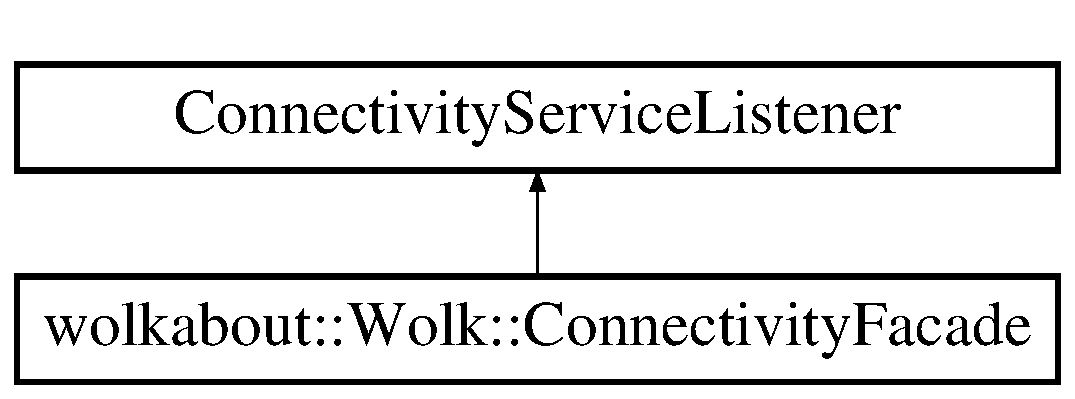
\includegraphics[height=2.000000cm]{classwolkabout_1_1_wolk_1_1_connectivity_facade}
\end{center}
\end{figure}
\subsection*{Public Member Functions}
\begin{DoxyCompactItemize}
\item 
\hyperlink{classwolkabout_1_1_wolk_1_1_connectivity_facade_a85471a9d7bf22254a6c083dceba55450}{Connectivity\+Facade} (Inbound\+Message\+Handler \&handler, std\+::function$<$ void()$>$ connection\+Lost\+Handler)
\item 
void \hyperlink{classwolkabout_1_1_wolk_1_1_connectivity_facade_a40bd02a3c7c65618f9662a4a4234f157}{message\+Received} (const std\+::string \&channel, const std\+::string \&message) override
\item 
void \hyperlink{classwolkabout_1_1_wolk_1_1_connectivity_facade_a16233edc1133bbb6dd19c19985674328}{connection\+Lost} () override
\item 
std\+::vector$<$ std\+::string $>$ \hyperlink{classwolkabout_1_1_wolk_1_1_connectivity_facade_a5494e952f413e2bcf0856d7ccf7dae86}{get\+Channels} () const override
\end{DoxyCompactItemize}
\subsection*{Private Attributes}
\begin{DoxyCompactItemize}
\item 
Inbound\+Message\+Handler \& \hyperlink{classwolkabout_1_1_wolk_1_1_connectivity_facade_a3bb32b6dccd5d889b96d4dd957d5466e}{m\+\_\+message\+Handler}
\item 
std\+::function$<$ void()$>$ \hyperlink{classwolkabout_1_1_wolk_1_1_connectivity_facade_abcb09f790a27656ce879445d147dd090}{m\+\_\+connection\+Lost\+Handler}
\end{DoxyCompactItemize}


\subsection{Constructor \& Destructor Documentation}
\index{wolkabout\+::\+Wolk\+::\+Connectivity\+Facade@{wolkabout\+::\+Wolk\+::\+Connectivity\+Facade}!Connectivity\+Facade@{Connectivity\+Facade}}
\index{Connectivity\+Facade@{Connectivity\+Facade}!wolkabout\+::\+Wolk\+::\+Connectivity\+Facade@{wolkabout\+::\+Wolk\+::\+Connectivity\+Facade}}
\subsubsection[{\texorpdfstring{Connectivity\+Facade(\+Inbound\+Message\+Handler \&handler, std\+::function$<$ void()$>$ connection\+Lost\+Handler)}{ConnectivityFacade(InboundMessageHandler &handler, std::function< void()> connectionLostHandler)}}]{\setlength{\rightskip}{0pt plus 5cm}wolkabout\+::\+Wolk\+::\+Connectivity\+Facade\+::\+Connectivity\+Facade (
\begin{DoxyParamCaption}
\item[{Inbound\+Message\+Handler \&}]{handler, }
\item[{std\+::function$<$ void()$>$}]{connection\+Lost\+Handler}
\end{DoxyParamCaption}
)}\hypertarget{classwolkabout_1_1_wolk_1_1_connectivity_facade_a85471a9d7bf22254a6c083dceba55450}{}\label{classwolkabout_1_1_wolk_1_1_connectivity_facade_a85471a9d7bf22254a6c083dceba55450}


\subsection{Member Function Documentation}
\index{wolkabout\+::\+Wolk\+::\+Connectivity\+Facade@{wolkabout\+::\+Wolk\+::\+Connectivity\+Facade}!connection\+Lost@{connection\+Lost}}
\index{connection\+Lost@{connection\+Lost}!wolkabout\+::\+Wolk\+::\+Connectivity\+Facade@{wolkabout\+::\+Wolk\+::\+Connectivity\+Facade}}
\subsubsection[{\texorpdfstring{connection\+Lost() override}{connectionLost() override}}]{\setlength{\rightskip}{0pt plus 5cm}void wolkabout\+::\+Wolk\+::\+Connectivity\+Facade\+::connection\+Lost (
\begin{DoxyParamCaption}
{}
\end{DoxyParamCaption}
)\hspace{0.3cm}{\ttfamily [override]}}\hypertarget{classwolkabout_1_1_wolk_1_1_connectivity_facade_a16233edc1133bbb6dd19c19985674328}{}\label{classwolkabout_1_1_wolk_1_1_connectivity_facade_a16233edc1133bbb6dd19c19985674328}
\index{wolkabout\+::\+Wolk\+::\+Connectivity\+Facade@{wolkabout\+::\+Wolk\+::\+Connectivity\+Facade}!get\+Channels@{get\+Channels}}
\index{get\+Channels@{get\+Channels}!wolkabout\+::\+Wolk\+::\+Connectivity\+Facade@{wolkabout\+::\+Wolk\+::\+Connectivity\+Facade}}
\subsubsection[{\texorpdfstring{get\+Channels() const override}{getChannels() const override}}]{\setlength{\rightskip}{0pt plus 5cm}std\+::vector$<$ std\+::string $>$ wolkabout\+::\+Wolk\+::\+Connectivity\+Facade\+::get\+Channels (
\begin{DoxyParamCaption}
{}
\end{DoxyParamCaption}
) const\hspace{0.3cm}{\ttfamily [override]}}\hypertarget{classwolkabout_1_1_wolk_1_1_connectivity_facade_a5494e952f413e2bcf0856d7ccf7dae86}{}\label{classwolkabout_1_1_wolk_1_1_connectivity_facade_a5494e952f413e2bcf0856d7ccf7dae86}
\index{wolkabout\+::\+Wolk\+::\+Connectivity\+Facade@{wolkabout\+::\+Wolk\+::\+Connectivity\+Facade}!message\+Received@{message\+Received}}
\index{message\+Received@{message\+Received}!wolkabout\+::\+Wolk\+::\+Connectivity\+Facade@{wolkabout\+::\+Wolk\+::\+Connectivity\+Facade}}
\subsubsection[{\texorpdfstring{message\+Received(const std\+::string \&channel, const std\+::string \&message) override}{messageReceived(const std::string &channel, const std::string &message) override}}]{\setlength{\rightskip}{0pt plus 5cm}void wolkabout\+::\+Wolk\+::\+Connectivity\+Facade\+::message\+Received (
\begin{DoxyParamCaption}
\item[{const std\+::string \&}]{channel, }
\item[{const std\+::string \&}]{message}
\end{DoxyParamCaption}
)\hspace{0.3cm}{\ttfamily [override]}}\hypertarget{classwolkabout_1_1_wolk_1_1_connectivity_facade_a40bd02a3c7c65618f9662a4a4234f157}{}\label{classwolkabout_1_1_wolk_1_1_connectivity_facade_a40bd02a3c7c65618f9662a4a4234f157}


\subsection{Member Data Documentation}
\index{wolkabout\+::\+Wolk\+::\+Connectivity\+Facade@{wolkabout\+::\+Wolk\+::\+Connectivity\+Facade}!m\+\_\+connection\+Lost\+Handler@{m\+\_\+connection\+Lost\+Handler}}
\index{m\+\_\+connection\+Lost\+Handler@{m\+\_\+connection\+Lost\+Handler}!wolkabout\+::\+Wolk\+::\+Connectivity\+Facade@{wolkabout\+::\+Wolk\+::\+Connectivity\+Facade}}
\subsubsection[{\texorpdfstring{m\+\_\+connection\+Lost\+Handler}{m_connectionLostHandler}}]{\setlength{\rightskip}{0pt plus 5cm}std\+::function$<$void()$>$ wolkabout\+::\+Wolk\+::\+Connectivity\+Facade\+::m\+\_\+connection\+Lost\+Handler\hspace{0.3cm}{\ttfamily [private]}}\hypertarget{classwolkabout_1_1_wolk_1_1_connectivity_facade_abcb09f790a27656ce879445d147dd090}{}\label{classwolkabout_1_1_wolk_1_1_connectivity_facade_abcb09f790a27656ce879445d147dd090}
\index{wolkabout\+::\+Wolk\+::\+Connectivity\+Facade@{wolkabout\+::\+Wolk\+::\+Connectivity\+Facade}!m\+\_\+message\+Handler@{m\+\_\+message\+Handler}}
\index{m\+\_\+message\+Handler@{m\+\_\+message\+Handler}!wolkabout\+::\+Wolk\+::\+Connectivity\+Facade@{wolkabout\+::\+Wolk\+::\+Connectivity\+Facade}}
\subsubsection[{\texorpdfstring{m\+\_\+message\+Handler}{m_messageHandler}}]{\setlength{\rightskip}{0pt plus 5cm}Inbound\+Message\+Handler\& wolkabout\+::\+Wolk\+::\+Connectivity\+Facade\+::m\+\_\+message\+Handler\hspace{0.3cm}{\ttfamily [private]}}\hypertarget{classwolkabout_1_1_wolk_1_1_connectivity_facade_a3bb32b6dccd5d889b96d4dd957d5466e}{}\label{classwolkabout_1_1_wolk_1_1_connectivity_facade_a3bb32b6dccd5d889b96d4dd957d5466e}


The documentation for this class was generated from the following files\+:\begin{DoxyCompactItemize}
\item 
src/\hyperlink{_wolk_8h}{Wolk.\+h}\item 
src/\hyperlink{_wolk_8cpp}{Wolk.\+cpp}\end{DoxyCompactItemize}

\hypertarget{classwolkabout_1_1_wolk}{}\section{wolkabout\+:\+:Wolk Class Reference}
\label{classwolkabout_1_1_wolk}\index{wolkabout\+::\+Wolk@{wolkabout\+::\+Wolk}}


{\ttfamily \#include $<$Wolk.\+h$>$}

\subsection*{Classes}
\begin{DoxyCompactItemize}
\item 
class \hyperlink{classwolkabout_1_1_wolk_1_1_connectivity_facade}{Connectivity\+Facade}
\end{DoxyCompactItemize}
\subsection*{Public Member Functions}
\begin{DoxyCompactItemize}
\item 
virtual \hyperlink{classwolkabout_1_1_wolk_a213707a5be879c29a5a32e7ae264e18e}{$\sim$\+Wolk} ()=default
\item 
{\footnotesize template$<$typename T $>$ }\\void \hyperlink{classwolkabout_1_1_wolk_a8b0e5e82c95c206361bc555091581721}{add\+Sensor\+Reading} (const std\+::string \&reference, T value, unsigned long long int rtc=0)
\begin{DoxyCompactList}\small\item\em Publishes sensor reading to Wolk\+About IoT Cloud~\newline
 This method is thread safe, and can be called from multiple thread simultaneously. \end{DoxyCompactList}\item 
{\footnotesize template$<$typename T $>$ }\\void \hyperlink{classwolkabout_1_1_wolk_a107e97d09b14a9ec270834b084aa57c0}{add\+Sensor\+Reading} (const std\+::string \&reference, std\+::initializer\+\_\+list$<$ T $>$ values, unsigned long long int rtc=0)
\begin{DoxyCompactList}\small\item\em Publishes multi-\/value sensor reading to Wolk\+About IoT Cloud~\newline
 This method is thread safe, and can be called from multiple thread simultaneously. \end{DoxyCompactList}\item 
{\footnotesize template$<$typename T $>$ }\\void \hyperlink{classwolkabout_1_1_wolk_a312f30b081b6d4a8f1bb7e2215de0e5d}{add\+Sensor\+Reading} (const std\+::string \&reference, const std\+::vector$<$ T $>$ values, unsigned long long int rtc=0)
\begin{DoxyCompactList}\small\item\em Publishes multi-\/value sensor reading to Wolk\+About IoT Cloud~\newline
 This method is thread safe, and can be called from multiple thread simultaneously. \end{DoxyCompactList}\item 
void \hyperlink{classwolkabout_1_1_wolk_a8bcc9b4aab0fde2de3483d5d2e09e557}{add\+Alarm} (const std\+::string \&reference, bool active, unsigned long long int rtc=0)
\begin{DoxyCompactList}\small\item\em Publishes alarm to Wolk\+About IoT Cloud~\newline
 This method is thread safe, and can be called from multiple thread simultaneously. \end{DoxyCompactList}\item 
void \hyperlink{classwolkabout_1_1_wolk_a44615f58380fb36be1f2c21c5423469a}{publish\+Actuator\+Status} (const std\+::string \&reference)
\begin{DoxyCompactList}\small\item\em Invokes Actuator\+Status\+Provider to obtain actuator status, and the publishes it.~\newline
 This method is thread safe, and can be called from multiple thread simultaneously. \end{DoxyCompactList}\item 
void \hyperlink{classwolkabout_1_1_wolk_a07c1144ebaf09975fa8e9d2cdc908fe5}{publish\+Configuration} ()
\begin{DoxyCompactList}\small\item\em Invokes Configuration\+Provider to obtain device configuration, and the publishes it.~\newline
 This method is thread safe, and can be called from multiple thread simultaneously. \end{DoxyCompactList}\item 
void \hyperlink{classwolkabout_1_1_wolk_ae78f0c33b71e8d33861de8547de1c311}{connect} ()
\begin{DoxyCompactList}\small\item\em Establishes connection with Wolk\+About IoT platform. \end{DoxyCompactList}\item 
void \hyperlink{classwolkabout_1_1_wolk_a805c8f842b1e4a480ac1a8bc1b6add06}{disconnect} ()
\begin{DoxyCompactList}\small\item\em Disconnects from Wolk\+About IoT platform. \end{DoxyCompactList}\item 
void \hyperlink{classwolkabout_1_1_wolk_a692525b11e983643eb12b2bdfc54d4cd}{publish} ()
\begin{DoxyCompactList}\small\item\em Publishes data. \end{DoxyCompactList}\item 
{\footnotesize template$<$typename T $>$ }\\void \hyperlink{classwolkabout_1_1_wolk_a882dcff4a9d9d51fd9d0e76edfd03d9e}{add\+Sensor\+Reading} (const std\+::string \&reference, T value, unsigned long long rtc)
\item 
{\footnotesize template$<$$>$ }\\void \hyperlink{classwolkabout_1_1_wolk_a4704e782ac13a380a6d7ccdbabb3847e}{add\+Sensor\+Reading} (const std\+::string \&reference, std\+::string value, unsigned long long rtc)
\item 
{\footnotesize template$<$$>$ }\\void \hyperlink{classwolkabout_1_1_wolk_ac55d5659566c66a513cdbb2e29833028}{add\+Sensor\+Reading} (const std\+::string \&reference, const std\+::vector$<$ std\+::string $>$ values, unsigned long long int rtc)
\end{DoxyCompactItemize}
\subsection*{Static Public Member Functions}
\begin{DoxyCompactItemize}
\item 
static \hyperlink{classwolkabout_1_1_wolk_builder}{Wolk\+Builder} \hyperlink{classwolkabout_1_1_wolk_a91270bb8552c2dee634e552111db4bb0}{new\+Builder} (Device device)
\begin{DoxyCompactList}\small\item\em Initiates \hyperlink{classwolkabout_1_1_wolk_builder}{wolkabout\+::\+Wolk\+Builder} that configures device to connect to Wolk\+About IoT Cloud. \end{DoxyCompactList}\end{DoxyCompactItemize}
\subsection*{Private Member Functions}
\begin{DoxyCompactItemize}
\item 
\hyperlink{classwolkabout_1_1_wolk_a41022de71360a1b15a7ea31cd2fb2359}{Wolk} (Device device)
\item 
void \hyperlink{classwolkabout_1_1_wolk_ae35585894387377feeb3a2733a9f97f2}{add\+To\+Command\+Buffer} (std\+::function$<$ void()$>$ command)
\item 
void \hyperlink{classwolkabout_1_1_wolk_a19a43047e89446b79eda7e9c698fea23}{flush\+Actuator\+Statuses} ()
\item 
void \hyperlink{classwolkabout_1_1_wolk_a1ec153b5a83bcd5ee6c0940963f8d104}{flush\+Alarms} ()
\item 
void \hyperlink{classwolkabout_1_1_wolk_af8d94d21e60b2a9d68e7274d98194069}{flush\+Sensor\+Readings} ()
\item 
void \hyperlink{classwolkabout_1_1_wolk_aadf1fc338b0c6f3e28b9c7285abce99b}{flush\+Configuration} ()
\item 
void \hyperlink{classwolkabout_1_1_wolk_aa56ee9c2d0ce80c90ed9e15d5304947b}{handle\+Actuator\+Set\+Command} (const std\+::string \&reference, const std\+::string \&value)
\item 
void \hyperlink{classwolkabout_1_1_wolk_a660c9c9ce35be66b1cedfb4a1e852858}{handle\+Actuator\+Get\+Command} (const std\+::string \&reference)
\item 
void \hyperlink{classwolkabout_1_1_wolk_ad2f16682dda7d5fe9ad86d9fadf51cd2}{handle\+Configuration\+Set\+Command} (const Configuration\+Set\+Command \&command)
\item 
void \hyperlink{classwolkabout_1_1_wolk_a1b64a9d38d23032da4e902ee8aa02bf5}{handle\+Configuration\+Get\+Command} ()
\item 
void \hyperlink{classwolkabout_1_1_wolk_a7e210f7d659cc5d390396710ef128e89}{publish\+Firmware\+Version} ()
\item 
std\+::string \hyperlink{classwolkabout_1_1_wolk_a71be75b9c18efa4912aaede25c9f1f4f}{get\+Sensor\+Delimiter} (const std\+::string \&reference)
\item 
std\+::map$<$ std\+::string, std\+::string $>$ \hyperlink{classwolkabout_1_1_wolk_a700e5f1f34057233c90da1c0380c7e3f}{get\+Configuration\+Delimiters} ()
\item 
void \hyperlink{classwolkabout_1_1_wolk_ae1876fe71977816804ce4ec857e95b31}{notify\+Connected} ()
\item 
void \hyperlink{classwolkabout_1_1_wolk_a86338fabbcc8a75991ce77786b23e118}{notify\+Disonnected} ()
\end{DoxyCompactItemize}
\subsection*{Static Private Member Functions}
\begin{DoxyCompactItemize}
\item 
static unsigned long long int \hyperlink{classwolkabout_1_1_wolk_af089e5381e328eea215a99164062b1ef}{current\+Rtc} ()
\end{DoxyCompactItemize}
\subsection*{Private Attributes}
\begin{DoxyCompactItemize}
\item 
Device \hyperlink{classwolkabout_1_1_wolk_a693a46fb484c06e1bf8ac771995420ef}{m\+\_\+device}
\item 
std\+::unique\+\_\+ptr$<$ Data\+Protocol $>$ \hyperlink{classwolkabout_1_1_wolk_a7a8acc5345a3d6fd3b7e92dca9d4649c}{m\+\_\+data\+Protocol}
\item 
std\+::unique\+\_\+ptr$<$ Status\+Protocol $>$ \hyperlink{classwolkabout_1_1_wolk_ab410d711778fd39cba66ebac0c6d1929}{m\+\_\+status\+Protocol}
\item 
std\+::unique\+\_\+ptr$<$ File\+Download\+Protocol $>$ \hyperlink{classwolkabout_1_1_wolk_a0cc964d56e1f921a29b99448c4b6af64}{m\+\_\+file\+Download\+Protocol}
\item 
std\+::unique\+\_\+ptr$<$ Firmware\+Update\+Protocol $>$ \hyperlink{classwolkabout_1_1_wolk_a7b180b579e0bdc7dd0d076c00feb886f}{m\+\_\+firmware\+Update\+Protocol}
\item 
std\+::unique\+\_\+ptr$<$ Connectivity\+Service $>$ \hyperlink{classwolkabout_1_1_wolk_a3b3f8b196063ea4808b7a374b225d97b}{m\+\_\+connectivity\+Service}
\item 
std\+::shared\+\_\+ptr$<$ Persistence $>$ \hyperlink{classwolkabout_1_1_wolk_a648fe96503a4f17efe4a6904d995633c}{m\+\_\+persistence}
\item 
std\+::unique\+\_\+ptr$<$ Inbound\+Message\+Handler $>$ \hyperlink{classwolkabout_1_1_wolk_a968a3f3c38c437876989c747d23d4c68}{m\+\_\+inbound\+Message\+Handler}
\item 
std\+::shared\+\_\+ptr$<$ \hyperlink{classwolkabout_1_1_wolk_1_1_connectivity_facade}{Connectivity\+Facade} $>$ \hyperlink{classwolkabout_1_1_wolk_a7f90b6701319c6a12d4519679e18f730}{m\+\_\+connectivity\+Manager}
\item 
std\+::shared\+\_\+ptr$<$ Data\+Service $>$ \hyperlink{classwolkabout_1_1_wolk_ae9dd0455d678445224ebbb7e73985577}{m\+\_\+data\+Service}
\item 
std\+::shared\+\_\+ptr$<$ File\+Download\+Service $>$ \hyperlink{classwolkabout_1_1_wolk_ab52986b0cbb0939f51f8f8d4d45dfab0}{m\+\_\+file\+Download\+Service}
\item 
std\+::shared\+\_\+ptr$<$ Firmware\+Update\+Service $>$ \hyperlink{classwolkabout_1_1_wolk_aa26f2abac76d31fd3a13f56cf5f8b20d}{m\+\_\+firmware\+Update\+Service}
\item 
std\+::shared\+\_\+ptr$<$ Keep\+Alive\+Service $>$ \hyperlink{classwolkabout_1_1_wolk_a03e41fa47eb856bfaab0adfc5e90770c}{m\+\_\+keep\+Alive\+Service}
\item 
std\+::function$<$ void(std\+::string, std\+::string)$>$ \hyperlink{classwolkabout_1_1_wolk_a0e261d8a574948ab3bed814de0a571da}{m\+\_\+actuation\+Handler\+Lambda}
\item 
std\+::weak\+\_\+ptr$<$ Actuation\+Handler $>$ \hyperlink{classwolkabout_1_1_wolk_a5995d8743c22d508c4dbba6e652f1244}{m\+\_\+actuation\+Handler}
\item 
std\+::function$<$ Actuator\+Status(std\+::string)$>$ \hyperlink{classwolkabout_1_1_wolk_a357c76819475203ea44f0deceb82f3bf}{m\+\_\+actuator\+Status\+Provider\+Lambda}
\item 
std\+::weak\+\_\+ptr$<$ Actuator\+Status\+Provider $>$ \hyperlink{classwolkabout_1_1_wolk_a77da2ea8914c67af1417b39b8c19b928}{m\+\_\+actuator\+Status\+Provider}
\item 
std\+::function$<$ void(const std\+::vector$<$ Configuration\+Item $>$ \&configuration)$>$ \hyperlink{classwolkabout_1_1_wolk_ae47e78eeb1e265a999014209d7bf15df}{m\+\_\+configuration\+Handler\+Lambda}
\item 
std\+::weak\+\_\+ptr$<$ Configuration\+Handler $>$ \hyperlink{classwolkabout_1_1_wolk_a662b0a47eb325a676adaf7bdd07a9c4d}{m\+\_\+configuration\+Handler}
\item 
std\+::function$<$ std\+::vector$<$ Configuration\+Item $>$)$>$ \hyperlink{classwolkabout_1_1_wolk_a0b022ee57d9ae6101b2868828e24b8c1}{m\+\_\+configuration\+Provider\+Lambda}
\item 
std\+::weak\+\_\+ptr$<$ Configuration\+Provider $>$ \hyperlink{classwolkabout_1_1_wolk_a31588377251dadbb584911fb30e9fe5d}{m\+\_\+configuration\+Provider}
\item 
std\+::unique\+\_\+ptr$<$ Command\+Buffer $>$ \hyperlink{classwolkabout_1_1_wolk_a84181505958620f03aa65303362c4103}{m\+\_\+command\+Buffer}
\end{DoxyCompactItemize}
\subsection*{Static Private Attributes}
\begin{DoxyCompactItemize}
\item 
static const constexpr unsigned int \hyperlink{classwolkabout_1_1_wolk_a4546eac23e520d87ab3e335740a044f3}{P\+U\+B\+L\+I\+S\+H\+\_\+\+B\+A\+T\+C\+H\+\_\+\+I\+T\+E\+M\+S\+\_\+\+C\+O\+U\+NT} = 50
\item 
static const constexpr std\+::chrono\+::seconds \hyperlink{classwolkabout_1_1_wolk_a0baa96b788266a9f9b164cd2e8799e73}{K\+E\+E\+P\+\_\+\+A\+L\+I\+V\+E\+\_\+\+I\+N\+T\+E\+R\+V\+AL} \{600\}
\end{DoxyCompactItemize}
\subsection*{Friends}
\begin{DoxyCompactItemize}
\item 
class \hyperlink{classwolkabout_1_1_wolk_aa7f95cb7914ddd6cb902a924d947cc1d}{Wolk\+Builder}
\end{DoxyCompactItemize}


\subsection{Constructor \& Destructor Documentation}
\index{wolkabout\+::\+Wolk@{wolkabout\+::\+Wolk}!````~Wolk@{$\sim$\+Wolk}}
\index{````~Wolk@{$\sim$\+Wolk}!wolkabout\+::\+Wolk@{wolkabout\+::\+Wolk}}
\subsubsection[{\texorpdfstring{$\sim$\+Wolk()=default}{~Wolk()=default}}]{\setlength{\rightskip}{0pt plus 5cm}virtual wolkabout\+::\+Wolk\+::$\sim$\+Wolk (
\begin{DoxyParamCaption}
{}
\end{DoxyParamCaption}
)\hspace{0.3cm}{\ttfamily [virtual]}, {\ttfamily [default]}}\hypertarget{classwolkabout_1_1_wolk_a213707a5be879c29a5a32e7ae264e18e}{}\label{classwolkabout_1_1_wolk_a213707a5be879c29a5a32e7ae264e18e}
\index{wolkabout\+::\+Wolk@{wolkabout\+::\+Wolk}!Wolk@{Wolk}}
\index{Wolk@{Wolk}!wolkabout\+::\+Wolk@{wolkabout\+::\+Wolk}}
\subsubsection[{\texorpdfstring{Wolk(\+Device device)}{Wolk(Device device)}}]{\setlength{\rightskip}{0pt plus 5cm}wolkabout\+::\+Wolk\+::\+Wolk (
\begin{DoxyParamCaption}
\item[{Device}]{device}
\end{DoxyParamCaption}
)\hspace{0.3cm}{\ttfamily [private]}}\hypertarget{classwolkabout_1_1_wolk_a41022de71360a1b15a7ea31cd2fb2359}{}\label{classwolkabout_1_1_wolk_a41022de71360a1b15a7ea31cd2fb2359}


\subsection{Member Function Documentation}
\index{wolkabout\+::\+Wolk@{wolkabout\+::\+Wolk}!add\+Alarm@{add\+Alarm}}
\index{add\+Alarm@{add\+Alarm}!wolkabout\+::\+Wolk@{wolkabout\+::\+Wolk}}
\subsubsection[{\texorpdfstring{add\+Alarm(const std\+::string \&reference, bool active, unsigned long long int rtc=0)}{addAlarm(const std::string &reference, bool active, unsigned long long int rtc=0)}}]{\setlength{\rightskip}{0pt plus 5cm}void wolkabout\+::\+Wolk\+::add\+Alarm (
\begin{DoxyParamCaption}
\item[{const std\+::string \&}]{reference, }
\item[{bool}]{active, }
\item[{unsigned long long int}]{rtc = {\ttfamily 0}}
\end{DoxyParamCaption}
)}\hypertarget{classwolkabout_1_1_wolk_a8bcc9b4aab0fde2de3483d5d2e09e557}{}\label{classwolkabout_1_1_wolk_a8bcc9b4aab0fde2de3483d5d2e09e557}


Publishes alarm to Wolk\+About IoT Cloud~\newline
 This method is thread safe, and can be called from multiple thread simultaneously. 


\begin{DoxyParams}{Parameters}
{\em reference} & Alarm reference \\
\hline
{\em active} & Is alarm active or not \\
\hline
{\em rtc} & P\+O\+S\+IX time at which event occurred -\/ Number of seconds since 01/01/1970~\newline
 If omitted current P\+O\+S\+IX time is adopted \\
\hline
\end{DoxyParams}
\index{wolkabout\+::\+Wolk@{wolkabout\+::\+Wolk}!add\+Sensor\+Reading@{add\+Sensor\+Reading}}
\index{add\+Sensor\+Reading@{add\+Sensor\+Reading}!wolkabout\+::\+Wolk@{wolkabout\+::\+Wolk}}
\subsubsection[{\texorpdfstring{add\+Sensor\+Reading(const std\+::string \&reference, T value, unsigned long long rtc)}{addSensorReading(const std::string &reference, T value, unsigned long long rtc)}}]{\setlength{\rightskip}{0pt plus 5cm}template$<$typename T $>$ void wolkabout\+::\+Wolk\+::add\+Sensor\+Reading (
\begin{DoxyParamCaption}
\item[{const std\+::string \&}]{reference, }
\item[{T}]{value, }
\item[{unsigned long long}]{rtc}
\end{DoxyParamCaption}
)}\hypertarget{classwolkabout_1_1_wolk_a882dcff4a9d9d51fd9d0e76edfd03d9e}{}\label{classwolkabout_1_1_wolk_a882dcff4a9d9d51fd9d0e76edfd03d9e}
\index{wolkabout\+::\+Wolk@{wolkabout\+::\+Wolk}!add\+Sensor\+Reading@{add\+Sensor\+Reading}}
\index{add\+Sensor\+Reading@{add\+Sensor\+Reading}!wolkabout\+::\+Wolk@{wolkabout\+::\+Wolk}}
\subsubsection[{\texorpdfstring{add\+Sensor\+Reading(const std\+::string \&reference, std\+::string value, unsigned long long rtc)}{addSensorReading(const std::string &reference, std::string value, unsigned long long rtc)}}]{\setlength{\rightskip}{0pt plus 5cm}template$<$$>$ void wolkabout\+::\+Wolk\+::add\+Sensor\+Reading (
\begin{DoxyParamCaption}
\item[{const std\+::string \&}]{reference, }
\item[{std\+::string}]{value, }
\item[{unsigned long long}]{rtc}
\end{DoxyParamCaption}
)}\hypertarget{classwolkabout_1_1_wolk_a4704e782ac13a380a6d7ccdbabb3847e}{}\label{classwolkabout_1_1_wolk_a4704e782ac13a380a6d7ccdbabb3847e}
\index{wolkabout\+::\+Wolk@{wolkabout\+::\+Wolk}!add\+Sensor\+Reading@{add\+Sensor\+Reading}}
\index{add\+Sensor\+Reading@{add\+Sensor\+Reading}!wolkabout\+::\+Wolk@{wolkabout\+::\+Wolk}}
\subsubsection[{\texorpdfstring{add\+Sensor\+Reading(const std\+::string \&reference, T value, unsigned long long int rtc=0)}{addSensorReading(const std::string &reference, T value, unsigned long long int rtc=0)}}]{\setlength{\rightskip}{0pt plus 5cm}template$<$typename T $>$ void wolkabout\+::\+Wolk\+::add\+Sensor\+Reading (
\begin{DoxyParamCaption}
\item[{const std\+::string \&}]{reference, }
\item[{T}]{value, }
\item[{unsigned long long int}]{rtc = {\ttfamily 0}}
\end{DoxyParamCaption}
)}\hypertarget{classwolkabout_1_1_wolk_a8b0e5e82c95c206361bc555091581721}{}\label{classwolkabout_1_1_wolk_a8b0e5e82c95c206361bc555091581721}


Publishes sensor reading to Wolk\+About IoT Cloud~\newline
 This method is thread safe, and can be called from multiple thread simultaneously. 


\begin{DoxyParams}{Parameters}
{\em reference} & Sensor reference \\
\hline
{\em value} & Sensor value~\newline
 Supported types\+:~\newline

\begin{DoxyItemize}
\item bool~\newline

\item float~\newline

\item double~\newline

\item signed int~\newline

\item signed long int~\newline

\item signed long long int~\newline

\item unsigned int~\newline

\item unsigned long int~\newline

\item unsigned long long int~\newline

\item string~\newline

\item char$\ast$~\newline

\item const char$\ast$~\newline
 
\end{DoxyItemize}\\
\hline
{\em rtc} & Reading P\+O\+S\+IX time -\/ Number of seconds since 01/01/1970~\newline
 If omitted current P\+O\+S\+IX time is adopted \\
\hline
\end{DoxyParams}
\index{wolkabout\+::\+Wolk@{wolkabout\+::\+Wolk}!add\+Sensor\+Reading@{add\+Sensor\+Reading}}
\index{add\+Sensor\+Reading@{add\+Sensor\+Reading}!wolkabout\+::\+Wolk@{wolkabout\+::\+Wolk}}
\subsubsection[{\texorpdfstring{add\+Sensor\+Reading(const std\+::string \&reference, const std\+::vector$<$ std\+::string $>$ values, unsigned long long int rtc)}{addSensorReading(const std::string &reference, const std::vector< std::string > values, unsigned long long int rtc)}}]{\setlength{\rightskip}{0pt plus 5cm}template$<$$>$ void wolkabout\+::\+Wolk\+::add\+Sensor\+Reading (
\begin{DoxyParamCaption}
\item[{const std\+::string \&}]{reference, }
\item[{const std\+::vector$<$ std\+::string $>$}]{values, }
\item[{unsigned long long int}]{rtc}
\end{DoxyParamCaption}
)}\hypertarget{classwolkabout_1_1_wolk_ac55d5659566c66a513cdbb2e29833028}{}\label{classwolkabout_1_1_wolk_ac55d5659566c66a513cdbb2e29833028}
\index{wolkabout\+::\+Wolk@{wolkabout\+::\+Wolk}!add\+Sensor\+Reading@{add\+Sensor\+Reading}}
\index{add\+Sensor\+Reading@{add\+Sensor\+Reading}!wolkabout\+::\+Wolk@{wolkabout\+::\+Wolk}}
\subsubsection[{\texorpdfstring{add\+Sensor\+Reading(const std\+::string \&reference, std\+::initializer\+\_\+list$<$ T $>$ values, unsigned long long int rtc=0)}{addSensorReading(const std::string &reference, std::initializer_list< T > values, unsigned long long int rtc=0)}}]{\setlength{\rightskip}{0pt plus 5cm}template$<$typename T $>$ void wolkabout\+::\+Wolk\+::add\+Sensor\+Reading (
\begin{DoxyParamCaption}
\item[{const std\+::string \&}]{reference, }
\item[{std\+::initializer\+\_\+list$<$ T $>$}]{values, }
\item[{unsigned long long int}]{rtc = {\ttfamily 0}}
\end{DoxyParamCaption}
)}\hypertarget{classwolkabout_1_1_wolk_a107e97d09b14a9ec270834b084aa57c0}{}\label{classwolkabout_1_1_wolk_a107e97d09b14a9ec270834b084aa57c0}


Publishes multi-\/value sensor reading to Wolk\+About IoT Cloud~\newline
 This method is thread safe, and can be called from multiple thread simultaneously. 


\begin{DoxyParams}{Parameters}
{\em reference} & Sensor reference \\
\hline
{\em values} & Multi-\/value sensor values~\newline
 Supported types\+:~\newline

\begin{DoxyItemize}
\item bool~\newline

\item float~\newline

\item double~\newline

\item signed int~\newline

\item signed long int~\newline

\item signed long long int~\newline

\item unsigned int~\newline

\item unsigned long int~\newline

\item unsigned long long int~\newline

\item string~\newline

\item char$\ast$~\newline

\item const char$\ast$~\newline
 
\end{DoxyItemize}\\
\hline
{\em rtc} & Reading P\+O\+S\+IX time -\/ Number of seconds since 01/01/1970~\newline
 If omitted current P\+O\+S\+IX time is adopted \\
\hline
\end{DoxyParams}
\index{wolkabout\+::\+Wolk@{wolkabout\+::\+Wolk}!add\+Sensor\+Reading@{add\+Sensor\+Reading}}
\index{add\+Sensor\+Reading@{add\+Sensor\+Reading}!wolkabout\+::\+Wolk@{wolkabout\+::\+Wolk}}
\subsubsection[{\texorpdfstring{add\+Sensor\+Reading(const std\+::string \&reference, const std\+::vector$<$ T $>$ values, unsigned long long int rtc=0)}{addSensorReading(const std::string &reference, const std::vector< T > values, unsigned long long int rtc=0)}}]{\setlength{\rightskip}{0pt plus 5cm}template$<$typename T $>$ void wolkabout\+::\+Wolk\+::add\+Sensor\+Reading (
\begin{DoxyParamCaption}
\item[{const std\+::string \&}]{reference, }
\item[{const std\+::vector$<$ T $>$}]{values, }
\item[{unsigned long long int}]{rtc = {\ttfamily 0}}
\end{DoxyParamCaption}
)}\hypertarget{classwolkabout_1_1_wolk_a312f30b081b6d4a8f1bb7e2215de0e5d}{}\label{classwolkabout_1_1_wolk_a312f30b081b6d4a8f1bb7e2215de0e5d}


Publishes multi-\/value sensor reading to Wolk\+About IoT Cloud~\newline
 This method is thread safe, and can be called from multiple thread simultaneously. 


\begin{DoxyParams}{Parameters}
{\em reference} & Sensor reference \\
\hline
{\em values} & Multi-\/value sensor values~\newline
 Supported types\+:~\newline

\begin{DoxyItemize}
\item bool~\newline

\item float~\newline

\item double~\newline

\item signed int~\newline

\item signed long int~\newline

\item signed long long int~\newline

\item unsigned int~\newline

\item unsigned long int~\newline

\item unsigned long long int~\newline

\item string~\newline

\item char$\ast$~\newline

\item const char$\ast$~\newline
 
\end{DoxyItemize}\\
\hline
{\em rtc} & Reading P\+O\+S\+IX time -\/ Number of seconds since 01/01/1970~\newline
 If omitted current P\+O\+S\+IX time is adopted \\
\hline
\end{DoxyParams}
\index{wolkabout\+::\+Wolk@{wolkabout\+::\+Wolk}!add\+To\+Command\+Buffer@{add\+To\+Command\+Buffer}}
\index{add\+To\+Command\+Buffer@{add\+To\+Command\+Buffer}!wolkabout\+::\+Wolk@{wolkabout\+::\+Wolk}}
\subsubsection[{\texorpdfstring{add\+To\+Command\+Buffer(std\+::function$<$ void()$>$ command)}{addToCommandBuffer(std::function< void()> command)}}]{\setlength{\rightskip}{0pt plus 5cm}void wolkabout\+::\+Wolk\+::add\+To\+Command\+Buffer (
\begin{DoxyParamCaption}
\item[{std\+::function$<$ void()$>$}]{command}
\end{DoxyParamCaption}
)\hspace{0.3cm}{\ttfamily [private]}}\hypertarget{classwolkabout_1_1_wolk_ae35585894387377feeb3a2733a9f97f2}{}\label{classwolkabout_1_1_wolk_ae35585894387377feeb3a2733a9f97f2}
\index{wolkabout\+::\+Wolk@{wolkabout\+::\+Wolk}!connect@{connect}}
\index{connect@{connect}!wolkabout\+::\+Wolk@{wolkabout\+::\+Wolk}}
\subsubsection[{\texorpdfstring{connect()}{connect()}}]{\setlength{\rightskip}{0pt plus 5cm}void wolkabout\+::\+Wolk\+::connect (
\begin{DoxyParamCaption}
{}
\end{DoxyParamCaption}
)}\hypertarget{classwolkabout_1_1_wolk_ae78f0c33b71e8d33861de8547de1c311}{}\label{classwolkabout_1_1_wolk_ae78f0c33b71e8d33861de8547de1c311}


Establishes connection with Wolk\+About IoT platform. 

\index{wolkabout\+::\+Wolk@{wolkabout\+::\+Wolk}!current\+Rtc@{current\+Rtc}}
\index{current\+Rtc@{current\+Rtc}!wolkabout\+::\+Wolk@{wolkabout\+::\+Wolk}}
\subsubsection[{\texorpdfstring{current\+Rtc()}{currentRtc()}}]{\setlength{\rightskip}{0pt plus 5cm}unsigned long long wolkabout\+::\+Wolk\+::current\+Rtc (
\begin{DoxyParamCaption}
{}
\end{DoxyParamCaption}
)\hspace{0.3cm}{\ttfamily [static]}, {\ttfamily [private]}}\hypertarget{classwolkabout_1_1_wolk_af089e5381e328eea215a99164062b1ef}{}\label{classwolkabout_1_1_wolk_af089e5381e328eea215a99164062b1ef}
\index{wolkabout\+::\+Wolk@{wolkabout\+::\+Wolk}!disconnect@{disconnect}}
\index{disconnect@{disconnect}!wolkabout\+::\+Wolk@{wolkabout\+::\+Wolk}}
\subsubsection[{\texorpdfstring{disconnect()}{disconnect()}}]{\setlength{\rightskip}{0pt plus 5cm}void wolkabout\+::\+Wolk\+::disconnect (
\begin{DoxyParamCaption}
{}
\end{DoxyParamCaption}
)}\hypertarget{classwolkabout_1_1_wolk_a805c8f842b1e4a480ac1a8bc1b6add06}{}\label{classwolkabout_1_1_wolk_a805c8f842b1e4a480ac1a8bc1b6add06}


Disconnects from Wolk\+About IoT platform. 

\index{wolkabout\+::\+Wolk@{wolkabout\+::\+Wolk}!flush\+Actuator\+Statuses@{flush\+Actuator\+Statuses}}
\index{flush\+Actuator\+Statuses@{flush\+Actuator\+Statuses}!wolkabout\+::\+Wolk@{wolkabout\+::\+Wolk}}
\subsubsection[{\texorpdfstring{flush\+Actuator\+Statuses()}{flushActuatorStatuses()}}]{\setlength{\rightskip}{0pt plus 5cm}void wolkabout\+::\+Wolk\+::flush\+Actuator\+Statuses (
\begin{DoxyParamCaption}
{}
\end{DoxyParamCaption}
)\hspace{0.3cm}{\ttfamily [private]}}\hypertarget{classwolkabout_1_1_wolk_a19a43047e89446b79eda7e9c698fea23}{}\label{classwolkabout_1_1_wolk_a19a43047e89446b79eda7e9c698fea23}
\index{wolkabout\+::\+Wolk@{wolkabout\+::\+Wolk}!flush\+Alarms@{flush\+Alarms}}
\index{flush\+Alarms@{flush\+Alarms}!wolkabout\+::\+Wolk@{wolkabout\+::\+Wolk}}
\subsubsection[{\texorpdfstring{flush\+Alarms()}{flushAlarms()}}]{\setlength{\rightskip}{0pt plus 5cm}void wolkabout\+::\+Wolk\+::flush\+Alarms (
\begin{DoxyParamCaption}
{}
\end{DoxyParamCaption}
)\hspace{0.3cm}{\ttfamily [private]}}\hypertarget{classwolkabout_1_1_wolk_a1ec153b5a83bcd5ee6c0940963f8d104}{}\label{classwolkabout_1_1_wolk_a1ec153b5a83bcd5ee6c0940963f8d104}
\index{wolkabout\+::\+Wolk@{wolkabout\+::\+Wolk}!flush\+Configuration@{flush\+Configuration}}
\index{flush\+Configuration@{flush\+Configuration}!wolkabout\+::\+Wolk@{wolkabout\+::\+Wolk}}
\subsubsection[{\texorpdfstring{flush\+Configuration()}{flushConfiguration()}}]{\setlength{\rightskip}{0pt plus 5cm}void wolkabout\+::\+Wolk\+::flush\+Configuration (
\begin{DoxyParamCaption}
{}
\end{DoxyParamCaption}
)\hspace{0.3cm}{\ttfamily [private]}}\hypertarget{classwolkabout_1_1_wolk_aadf1fc338b0c6f3e28b9c7285abce99b}{}\label{classwolkabout_1_1_wolk_aadf1fc338b0c6f3e28b9c7285abce99b}
\index{wolkabout\+::\+Wolk@{wolkabout\+::\+Wolk}!flush\+Sensor\+Readings@{flush\+Sensor\+Readings}}
\index{flush\+Sensor\+Readings@{flush\+Sensor\+Readings}!wolkabout\+::\+Wolk@{wolkabout\+::\+Wolk}}
\subsubsection[{\texorpdfstring{flush\+Sensor\+Readings()}{flushSensorReadings()}}]{\setlength{\rightskip}{0pt plus 5cm}void wolkabout\+::\+Wolk\+::flush\+Sensor\+Readings (
\begin{DoxyParamCaption}
{}
\end{DoxyParamCaption}
)\hspace{0.3cm}{\ttfamily [private]}}\hypertarget{classwolkabout_1_1_wolk_af8d94d21e60b2a9d68e7274d98194069}{}\label{classwolkabout_1_1_wolk_af8d94d21e60b2a9d68e7274d98194069}
\index{wolkabout\+::\+Wolk@{wolkabout\+::\+Wolk}!get\+Configuration\+Delimiters@{get\+Configuration\+Delimiters}}
\index{get\+Configuration\+Delimiters@{get\+Configuration\+Delimiters}!wolkabout\+::\+Wolk@{wolkabout\+::\+Wolk}}
\subsubsection[{\texorpdfstring{get\+Configuration\+Delimiters()}{getConfigurationDelimiters()}}]{\setlength{\rightskip}{0pt plus 5cm}std\+::map$<$ std\+::string, std\+::string $>$ wolkabout\+::\+Wolk\+::get\+Configuration\+Delimiters (
\begin{DoxyParamCaption}
{}
\end{DoxyParamCaption}
)\hspace{0.3cm}{\ttfamily [private]}}\hypertarget{classwolkabout_1_1_wolk_a700e5f1f34057233c90da1c0380c7e3f}{}\label{classwolkabout_1_1_wolk_a700e5f1f34057233c90da1c0380c7e3f}
\index{wolkabout\+::\+Wolk@{wolkabout\+::\+Wolk}!get\+Sensor\+Delimiter@{get\+Sensor\+Delimiter}}
\index{get\+Sensor\+Delimiter@{get\+Sensor\+Delimiter}!wolkabout\+::\+Wolk@{wolkabout\+::\+Wolk}}
\subsubsection[{\texorpdfstring{get\+Sensor\+Delimiter(const std\+::string \&reference)}{getSensorDelimiter(const std::string &reference)}}]{\setlength{\rightskip}{0pt plus 5cm}std\+::string wolkabout\+::\+Wolk\+::get\+Sensor\+Delimiter (
\begin{DoxyParamCaption}
\item[{const std\+::string \&}]{reference}
\end{DoxyParamCaption}
)\hspace{0.3cm}{\ttfamily [private]}}\hypertarget{classwolkabout_1_1_wolk_a71be75b9c18efa4912aaede25c9f1f4f}{}\label{classwolkabout_1_1_wolk_a71be75b9c18efa4912aaede25c9f1f4f}
\index{wolkabout\+::\+Wolk@{wolkabout\+::\+Wolk}!handle\+Actuator\+Get\+Command@{handle\+Actuator\+Get\+Command}}
\index{handle\+Actuator\+Get\+Command@{handle\+Actuator\+Get\+Command}!wolkabout\+::\+Wolk@{wolkabout\+::\+Wolk}}
\subsubsection[{\texorpdfstring{handle\+Actuator\+Get\+Command(const std\+::string \&reference)}{handleActuatorGetCommand(const std::string &reference)}}]{\setlength{\rightskip}{0pt plus 5cm}void wolkabout\+::\+Wolk\+::handle\+Actuator\+Get\+Command (
\begin{DoxyParamCaption}
\item[{const std\+::string \&}]{reference}
\end{DoxyParamCaption}
)\hspace{0.3cm}{\ttfamily [private]}}\hypertarget{classwolkabout_1_1_wolk_a660c9c9ce35be66b1cedfb4a1e852858}{}\label{classwolkabout_1_1_wolk_a660c9c9ce35be66b1cedfb4a1e852858}
\index{wolkabout\+::\+Wolk@{wolkabout\+::\+Wolk}!handle\+Actuator\+Set\+Command@{handle\+Actuator\+Set\+Command}}
\index{handle\+Actuator\+Set\+Command@{handle\+Actuator\+Set\+Command}!wolkabout\+::\+Wolk@{wolkabout\+::\+Wolk}}
\subsubsection[{\texorpdfstring{handle\+Actuator\+Set\+Command(const std\+::string \&reference, const std\+::string \&value)}{handleActuatorSetCommand(const std::string &reference, const std::string &value)}}]{\setlength{\rightskip}{0pt plus 5cm}void wolkabout\+::\+Wolk\+::handle\+Actuator\+Set\+Command (
\begin{DoxyParamCaption}
\item[{const std\+::string \&}]{reference, }
\item[{const std\+::string \&}]{value}
\end{DoxyParamCaption}
)\hspace{0.3cm}{\ttfamily [private]}}\hypertarget{classwolkabout_1_1_wolk_aa56ee9c2d0ce80c90ed9e15d5304947b}{}\label{classwolkabout_1_1_wolk_aa56ee9c2d0ce80c90ed9e15d5304947b}
\index{wolkabout\+::\+Wolk@{wolkabout\+::\+Wolk}!handle\+Configuration\+Get\+Command@{handle\+Configuration\+Get\+Command}}
\index{handle\+Configuration\+Get\+Command@{handle\+Configuration\+Get\+Command}!wolkabout\+::\+Wolk@{wolkabout\+::\+Wolk}}
\subsubsection[{\texorpdfstring{handle\+Configuration\+Get\+Command()}{handleConfigurationGetCommand()}}]{\setlength{\rightskip}{0pt plus 5cm}void wolkabout\+::\+Wolk\+::handle\+Configuration\+Get\+Command (
\begin{DoxyParamCaption}
{}
\end{DoxyParamCaption}
)\hspace{0.3cm}{\ttfamily [private]}}\hypertarget{classwolkabout_1_1_wolk_a1b64a9d38d23032da4e902ee8aa02bf5}{}\label{classwolkabout_1_1_wolk_a1b64a9d38d23032da4e902ee8aa02bf5}
\index{wolkabout\+::\+Wolk@{wolkabout\+::\+Wolk}!handle\+Configuration\+Set\+Command@{handle\+Configuration\+Set\+Command}}
\index{handle\+Configuration\+Set\+Command@{handle\+Configuration\+Set\+Command}!wolkabout\+::\+Wolk@{wolkabout\+::\+Wolk}}
\subsubsection[{\texorpdfstring{handle\+Configuration\+Set\+Command(const Configuration\+Set\+Command \&command)}{handleConfigurationSetCommand(const ConfigurationSetCommand &command)}}]{\setlength{\rightskip}{0pt plus 5cm}void wolkabout\+::\+Wolk\+::handle\+Configuration\+Set\+Command (
\begin{DoxyParamCaption}
\item[{const Configuration\+Set\+Command \&}]{command}
\end{DoxyParamCaption}
)\hspace{0.3cm}{\ttfamily [private]}}\hypertarget{classwolkabout_1_1_wolk_ad2f16682dda7d5fe9ad86d9fadf51cd2}{}\label{classwolkabout_1_1_wolk_ad2f16682dda7d5fe9ad86d9fadf51cd2}
\index{wolkabout\+::\+Wolk@{wolkabout\+::\+Wolk}!new\+Builder@{new\+Builder}}
\index{new\+Builder@{new\+Builder}!wolkabout\+::\+Wolk@{wolkabout\+::\+Wolk}}
\subsubsection[{\texorpdfstring{new\+Builder(\+Device device)}{newBuilder(Device device)}}]{\setlength{\rightskip}{0pt plus 5cm}{\bf Wolk\+Builder} wolkabout\+::\+Wolk\+::new\+Builder (
\begin{DoxyParamCaption}
\item[{Device}]{device}
\end{DoxyParamCaption}
)\hspace{0.3cm}{\ttfamily [static]}}\hypertarget{classwolkabout_1_1_wolk_a91270bb8552c2dee634e552111db4bb0}{}\label{classwolkabout_1_1_wolk_a91270bb8552c2dee634e552111db4bb0}


Initiates \hyperlink{classwolkabout_1_1_wolk_builder}{wolkabout\+::\+Wolk\+Builder} that configures device to connect to Wolk\+About IoT Cloud. 


\begin{DoxyParams}{Parameters}
{\em device} & wolkabout\+::\+Device \\
\hline
\end{DoxyParams}
\begin{DoxyReturn}{Returns}
\hyperlink{classwolkabout_1_1_wolk_builder}{wolkabout\+::\+Wolk\+Builder} instance 
\end{DoxyReturn}
\index{wolkabout\+::\+Wolk@{wolkabout\+::\+Wolk}!notify\+Connected@{notify\+Connected}}
\index{notify\+Connected@{notify\+Connected}!wolkabout\+::\+Wolk@{wolkabout\+::\+Wolk}}
\subsubsection[{\texorpdfstring{notify\+Connected()}{notifyConnected()}}]{\setlength{\rightskip}{0pt plus 5cm}void wolkabout\+::\+Wolk\+::notify\+Connected (
\begin{DoxyParamCaption}
{}
\end{DoxyParamCaption}
)\hspace{0.3cm}{\ttfamily [private]}}\hypertarget{classwolkabout_1_1_wolk_ae1876fe71977816804ce4ec857e95b31}{}\label{classwolkabout_1_1_wolk_ae1876fe71977816804ce4ec857e95b31}
\index{wolkabout\+::\+Wolk@{wolkabout\+::\+Wolk}!notify\+Disonnected@{notify\+Disonnected}}
\index{notify\+Disonnected@{notify\+Disonnected}!wolkabout\+::\+Wolk@{wolkabout\+::\+Wolk}}
\subsubsection[{\texorpdfstring{notify\+Disonnected()}{notifyDisonnected()}}]{\setlength{\rightskip}{0pt plus 5cm}void wolkabout\+::\+Wolk\+::notify\+Disonnected (
\begin{DoxyParamCaption}
{}
\end{DoxyParamCaption}
)\hspace{0.3cm}{\ttfamily [private]}}\hypertarget{classwolkabout_1_1_wolk_a86338fabbcc8a75991ce77786b23e118}{}\label{classwolkabout_1_1_wolk_a86338fabbcc8a75991ce77786b23e118}
\index{wolkabout\+::\+Wolk@{wolkabout\+::\+Wolk}!publish@{publish}}
\index{publish@{publish}!wolkabout\+::\+Wolk@{wolkabout\+::\+Wolk}}
\subsubsection[{\texorpdfstring{publish()}{publish()}}]{\setlength{\rightskip}{0pt plus 5cm}void wolkabout\+::\+Wolk\+::publish (
\begin{DoxyParamCaption}
{}
\end{DoxyParamCaption}
)}\hypertarget{classwolkabout_1_1_wolk_a692525b11e983643eb12b2bdfc54d4cd}{}\label{classwolkabout_1_1_wolk_a692525b11e983643eb12b2bdfc54d4cd}


Publishes data. 

\index{wolkabout\+::\+Wolk@{wolkabout\+::\+Wolk}!publish\+Actuator\+Status@{publish\+Actuator\+Status}}
\index{publish\+Actuator\+Status@{publish\+Actuator\+Status}!wolkabout\+::\+Wolk@{wolkabout\+::\+Wolk}}
\subsubsection[{\texorpdfstring{publish\+Actuator\+Status(const std\+::string \&reference)}{publishActuatorStatus(const std::string &reference)}}]{\setlength{\rightskip}{0pt plus 5cm}void wolkabout\+::\+Wolk\+::publish\+Actuator\+Status (
\begin{DoxyParamCaption}
\item[{const std\+::string \&}]{reference}
\end{DoxyParamCaption}
)}\hypertarget{classwolkabout_1_1_wolk_a44615f58380fb36be1f2c21c5423469a}{}\label{classwolkabout_1_1_wolk_a44615f58380fb36be1f2c21c5423469a}


Invokes Actuator\+Status\+Provider to obtain actuator status, and the publishes it.~\newline
 This method is thread safe, and can be called from multiple thread simultaneously. 


\begin{DoxyParams}{Parameters}
{\em Actuator} & reference \\
\hline
\end{DoxyParams}
\index{wolkabout\+::\+Wolk@{wolkabout\+::\+Wolk}!publish\+Configuration@{publish\+Configuration}}
\index{publish\+Configuration@{publish\+Configuration}!wolkabout\+::\+Wolk@{wolkabout\+::\+Wolk}}
\subsubsection[{\texorpdfstring{publish\+Configuration()}{publishConfiguration()}}]{\setlength{\rightskip}{0pt plus 5cm}void wolkabout\+::\+Wolk\+::publish\+Configuration (
\begin{DoxyParamCaption}
{}
\end{DoxyParamCaption}
)}\hypertarget{classwolkabout_1_1_wolk_a07c1144ebaf09975fa8e9d2cdc908fe5}{}\label{classwolkabout_1_1_wolk_a07c1144ebaf09975fa8e9d2cdc908fe5}


Invokes Configuration\+Provider to obtain device configuration, and the publishes it.~\newline
 This method is thread safe, and can be called from multiple thread simultaneously. 

\index{wolkabout\+::\+Wolk@{wolkabout\+::\+Wolk}!publish\+Firmware\+Version@{publish\+Firmware\+Version}}
\index{publish\+Firmware\+Version@{publish\+Firmware\+Version}!wolkabout\+::\+Wolk@{wolkabout\+::\+Wolk}}
\subsubsection[{\texorpdfstring{publish\+Firmware\+Version()}{publishFirmwareVersion()}}]{\setlength{\rightskip}{0pt plus 5cm}void wolkabout\+::\+Wolk\+::publish\+Firmware\+Version (
\begin{DoxyParamCaption}
{}
\end{DoxyParamCaption}
)\hspace{0.3cm}{\ttfamily [private]}}\hypertarget{classwolkabout_1_1_wolk_a7e210f7d659cc5d390396710ef128e89}{}\label{classwolkabout_1_1_wolk_a7e210f7d659cc5d390396710ef128e89}


\subsection{Friends And Related Function Documentation}
\index{wolkabout\+::\+Wolk@{wolkabout\+::\+Wolk}!Wolk\+Builder@{Wolk\+Builder}}
\index{Wolk\+Builder@{Wolk\+Builder}!wolkabout\+::\+Wolk@{wolkabout\+::\+Wolk}}
\subsubsection[{\texorpdfstring{Wolk\+Builder}{WolkBuilder}}]{\setlength{\rightskip}{0pt plus 5cm}friend class {\bf Wolk\+Builder}\hspace{0.3cm}{\ttfamily [friend]}}\hypertarget{classwolkabout_1_1_wolk_aa7f95cb7914ddd6cb902a924d947cc1d}{}\label{classwolkabout_1_1_wolk_aa7f95cb7914ddd6cb902a924d947cc1d}


\subsection{Member Data Documentation}
\index{wolkabout\+::\+Wolk@{wolkabout\+::\+Wolk}!K\+E\+E\+P\+\_\+\+A\+L\+I\+V\+E\+\_\+\+I\+N\+T\+E\+R\+V\+AL@{K\+E\+E\+P\+\_\+\+A\+L\+I\+V\+E\+\_\+\+I\+N\+T\+E\+R\+V\+AL}}
\index{K\+E\+E\+P\+\_\+\+A\+L\+I\+V\+E\+\_\+\+I\+N\+T\+E\+R\+V\+AL@{K\+E\+E\+P\+\_\+\+A\+L\+I\+V\+E\+\_\+\+I\+N\+T\+E\+R\+V\+AL}!wolkabout\+::\+Wolk@{wolkabout\+::\+Wolk}}
\subsubsection[{\texorpdfstring{K\+E\+E\+P\+\_\+\+A\+L\+I\+V\+E\+\_\+\+I\+N\+T\+E\+R\+V\+AL}{KEEP_ALIVE_INTERVAL}}]{\setlength{\rightskip}{0pt plus 5cm}const constexpr std\+::chrono\+::seconds wolkabout\+::\+Wolk\+::\+K\+E\+E\+P\+\_\+\+A\+L\+I\+V\+E\+\_\+\+I\+N\+T\+E\+R\+V\+AL \{600\}\hspace{0.3cm}{\ttfamily [static]}, {\ttfamily [private]}}\hypertarget{classwolkabout_1_1_wolk_a0baa96b788266a9f9b164cd2e8799e73}{}\label{classwolkabout_1_1_wolk_a0baa96b788266a9f9b164cd2e8799e73}
\index{wolkabout\+::\+Wolk@{wolkabout\+::\+Wolk}!m\+\_\+actuation\+Handler@{m\+\_\+actuation\+Handler}}
\index{m\+\_\+actuation\+Handler@{m\+\_\+actuation\+Handler}!wolkabout\+::\+Wolk@{wolkabout\+::\+Wolk}}
\subsubsection[{\texorpdfstring{m\+\_\+actuation\+Handler}{m_actuationHandler}}]{\setlength{\rightskip}{0pt plus 5cm}std\+::weak\+\_\+ptr$<$Actuation\+Handler$>$ wolkabout\+::\+Wolk\+::m\+\_\+actuation\+Handler\hspace{0.3cm}{\ttfamily [private]}}\hypertarget{classwolkabout_1_1_wolk_a5995d8743c22d508c4dbba6e652f1244}{}\label{classwolkabout_1_1_wolk_a5995d8743c22d508c4dbba6e652f1244}
\index{wolkabout\+::\+Wolk@{wolkabout\+::\+Wolk}!m\+\_\+actuation\+Handler\+Lambda@{m\+\_\+actuation\+Handler\+Lambda}}
\index{m\+\_\+actuation\+Handler\+Lambda@{m\+\_\+actuation\+Handler\+Lambda}!wolkabout\+::\+Wolk@{wolkabout\+::\+Wolk}}
\subsubsection[{\texorpdfstring{m\+\_\+actuation\+Handler\+Lambda}{m_actuationHandlerLambda}}]{\setlength{\rightskip}{0pt plus 5cm}std\+::function$<$void(std\+::string, std\+::string)$>$ wolkabout\+::\+Wolk\+::m\+\_\+actuation\+Handler\+Lambda\hspace{0.3cm}{\ttfamily [private]}}\hypertarget{classwolkabout_1_1_wolk_a0e261d8a574948ab3bed814de0a571da}{}\label{classwolkabout_1_1_wolk_a0e261d8a574948ab3bed814de0a571da}
\index{wolkabout\+::\+Wolk@{wolkabout\+::\+Wolk}!m\+\_\+actuator\+Status\+Provider@{m\+\_\+actuator\+Status\+Provider}}
\index{m\+\_\+actuator\+Status\+Provider@{m\+\_\+actuator\+Status\+Provider}!wolkabout\+::\+Wolk@{wolkabout\+::\+Wolk}}
\subsubsection[{\texorpdfstring{m\+\_\+actuator\+Status\+Provider}{m_actuatorStatusProvider}}]{\setlength{\rightskip}{0pt plus 5cm}std\+::weak\+\_\+ptr$<$Actuator\+Status\+Provider$>$ wolkabout\+::\+Wolk\+::m\+\_\+actuator\+Status\+Provider\hspace{0.3cm}{\ttfamily [private]}}\hypertarget{classwolkabout_1_1_wolk_a77da2ea8914c67af1417b39b8c19b928}{}\label{classwolkabout_1_1_wolk_a77da2ea8914c67af1417b39b8c19b928}
\index{wolkabout\+::\+Wolk@{wolkabout\+::\+Wolk}!m\+\_\+actuator\+Status\+Provider\+Lambda@{m\+\_\+actuator\+Status\+Provider\+Lambda}}
\index{m\+\_\+actuator\+Status\+Provider\+Lambda@{m\+\_\+actuator\+Status\+Provider\+Lambda}!wolkabout\+::\+Wolk@{wolkabout\+::\+Wolk}}
\subsubsection[{\texorpdfstring{m\+\_\+actuator\+Status\+Provider\+Lambda}{m_actuatorStatusProviderLambda}}]{\setlength{\rightskip}{0pt plus 5cm}std\+::function$<$Actuator\+Status(std\+::string)$>$ wolkabout\+::\+Wolk\+::m\+\_\+actuator\+Status\+Provider\+Lambda\hspace{0.3cm}{\ttfamily [private]}}\hypertarget{classwolkabout_1_1_wolk_a357c76819475203ea44f0deceb82f3bf}{}\label{classwolkabout_1_1_wolk_a357c76819475203ea44f0deceb82f3bf}
\index{wolkabout\+::\+Wolk@{wolkabout\+::\+Wolk}!m\+\_\+command\+Buffer@{m\+\_\+command\+Buffer}}
\index{m\+\_\+command\+Buffer@{m\+\_\+command\+Buffer}!wolkabout\+::\+Wolk@{wolkabout\+::\+Wolk}}
\subsubsection[{\texorpdfstring{m\+\_\+command\+Buffer}{m_commandBuffer}}]{\setlength{\rightskip}{0pt plus 5cm}std\+::unique\+\_\+ptr$<$Command\+Buffer$>$ wolkabout\+::\+Wolk\+::m\+\_\+command\+Buffer\hspace{0.3cm}{\ttfamily [private]}}\hypertarget{classwolkabout_1_1_wolk_a84181505958620f03aa65303362c4103}{}\label{classwolkabout_1_1_wolk_a84181505958620f03aa65303362c4103}
\index{wolkabout\+::\+Wolk@{wolkabout\+::\+Wolk}!m\+\_\+configuration\+Handler@{m\+\_\+configuration\+Handler}}
\index{m\+\_\+configuration\+Handler@{m\+\_\+configuration\+Handler}!wolkabout\+::\+Wolk@{wolkabout\+::\+Wolk}}
\subsubsection[{\texorpdfstring{m\+\_\+configuration\+Handler}{m_configurationHandler}}]{\setlength{\rightskip}{0pt plus 5cm}std\+::weak\+\_\+ptr$<$Configuration\+Handler$>$ wolkabout\+::\+Wolk\+::m\+\_\+configuration\+Handler\hspace{0.3cm}{\ttfamily [private]}}\hypertarget{classwolkabout_1_1_wolk_a662b0a47eb325a676adaf7bdd07a9c4d}{}\label{classwolkabout_1_1_wolk_a662b0a47eb325a676adaf7bdd07a9c4d}
\index{wolkabout\+::\+Wolk@{wolkabout\+::\+Wolk}!m\+\_\+configuration\+Handler\+Lambda@{m\+\_\+configuration\+Handler\+Lambda}}
\index{m\+\_\+configuration\+Handler\+Lambda@{m\+\_\+configuration\+Handler\+Lambda}!wolkabout\+::\+Wolk@{wolkabout\+::\+Wolk}}
\subsubsection[{\texorpdfstring{m\+\_\+configuration\+Handler\+Lambda}{m_configurationHandlerLambda}}]{\setlength{\rightskip}{0pt plus 5cm}std\+::function$<$void(const std\+::vector$<$Configuration\+Item$>$\& configuration)$>$ wolkabout\+::\+Wolk\+::m\+\_\+configuration\+Handler\+Lambda\hspace{0.3cm}{\ttfamily [private]}}\hypertarget{classwolkabout_1_1_wolk_ae47e78eeb1e265a999014209d7bf15df}{}\label{classwolkabout_1_1_wolk_ae47e78eeb1e265a999014209d7bf15df}
\index{wolkabout\+::\+Wolk@{wolkabout\+::\+Wolk}!m\+\_\+configuration\+Provider@{m\+\_\+configuration\+Provider}}
\index{m\+\_\+configuration\+Provider@{m\+\_\+configuration\+Provider}!wolkabout\+::\+Wolk@{wolkabout\+::\+Wolk}}
\subsubsection[{\texorpdfstring{m\+\_\+configuration\+Provider}{m_configurationProvider}}]{\setlength{\rightskip}{0pt plus 5cm}std\+::weak\+\_\+ptr$<$Configuration\+Provider$>$ wolkabout\+::\+Wolk\+::m\+\_\+configuration\+Provider\hspace{0.3cm}{\ttfamily [private]}}\hypertarget{classwolkabout_1_1_wolk_a31588377251dadbb584911fb30e9fe5d}{}\label{classwolkabout_1_1_wolk_a31588377251dadbb584911fb30e9fe5d}
\index{wolkabout\+::\+Wolk@{wolkabout\+::\+Wolk}!m\+\_\+configuration\+Provider\+Lambda@{m\+\_\+configuration\+Provider\+Lambda}}
\index{m\+\_\+configuration\+Provider\+Lambda@{m\+\_\+configuration\+Provider\+Lambda}!wolkabout\+::\+Wolk@{wolkabout\+::\+Wolk}}
\subsubsection[{\texorpdfstring{m\+\_\+configuration\+Provider\+Lambda}{m_configurationProviderLambda}}]{\setlength{\rightskip}{0pt plus 5cm}std\+::function$<$std\+::vector$<$Configuration\+Item$>$)$>$ wolkabout\+::\+Wolk\+::m\+\_\+configuration\+Provider\+Lambda\hspace{0.3cm}{\ttfamily [private]}}\hypertarget{classwolkabout_1_1_wolk_a0b022ee57d9ae6101b2868828e24b8c1}{}\label{classwolkabout_1_1_wolk_a0b022ee57d9ae6101b2868828e24b8c1}
\index{wolkabout\+::\+Wolk@{wolkabout\+::\+Wolk}!m\+\_\+connectivity\+Manager@{m\+\_\+connectivity\+Manager}}
\index{m\+\_\+connectivity\+Manager@{m\+\_\+connectivity\+Manager}!wolkabout\+::\+Wolk@{wolkabout\+::\+Wolk}}
\subsubsection[{\texorpdfstring{m\+\_\+connectivity\+Manager}{m_connectivityManager}}]{\setlength{\rightskip}{0pt plus 5cm}std\+::shared\+\_\+ptr$<${\bf Connectivity\+Facade}$>$ wolkabout\+::\+Wolk\+::m\+\_\+connectivity\+Manager\hspace{0.3cm}{\ttfamily [private]}}\hypertarget{classwolkabout_1_1_wolk_a7f90b6701319c6a12d4519679e18f730}{}\label{classwolkabout_1_1_wolk_a7f90b6701319c6a12d4519679e18f730}
\index{wolkabout\+::\+Wolk@{wolkabout\+::\+Wolk}!m\+\_\+connectivity\+Service@{m\+\_\+connectivity\+Service}}
\index{m\+\_\+connectivity\+Service@{m\+\_\+connectivity\+Service}!wolkabout\+::\+Wolk@{wolkabout\+::\+Wolk}}
\subsubsection[{\texorpdfstring{m\+\_\+connectivity\+Service}{m_connectivityService}}]{\setlength{\rightskip}{0pt plus 5cm}std\+::unique\+\_\+ptr$<$Connectivity\+Service$>$ wolkabout\+::\+Wolk\+::m\+\_\+connectivity\+Service\hspace{0.3cm}{\ttfamily [private]}}\hypertarget{classwolkabout_1_1_wolk_a3b3f8b196063ea4808b7a374b225d97b}{}\label{classwolkabout_1_1_wolk_a3b3f8b196063ea4808b7a374b225d97b}
\index{wolkabout\+::\+Wolk@{wolkabout\+::\+Wolk}!m\+\_\+data\+Protocol@{m\+\_\+data\+Protocol}}
\index{m\+\_\+data\+Protocol@{m\+\_\+data\+Protocol}!wolkabout\+::\+Wolk@{wolkabout\+::\+Wolk}}
\subsubsection[{\texorpdfstring{m\+\_\+data\+Protocol}{m_dataProtocol}}]{\setlength{\rightskip}{0pt plus 5cm}std\+::unique\+\_\+ptr$<$Data\+Protocol$>$ wolkabout\+::\+Wolk\+::m\+\_\+data\+Protocol\hspace{0.3cm}{\ttfamily [private]}}\hypertarget{classwolkabout_1_1_wolk_a7a8acc5345a3d6fd3b7e92dca9d4649c}{}\label{classwolkabout_1_1_wolk_a7a8acc5345a3d6fd3b7e92dca9d4649c}
\index{wolkabout\+::\+Wolk@{wolkabout\+::\+Wolk}!m\+\_\+data\+Service@{m\+\_\+data\+Service}}
\index{m\+\_\+data\+Service@{m\+\_\+data\+Service}!wolkabout\+::\+Wolk@{wolkabout\+::\+Wolk}}
\subsubsection[{\texorpdfstring{m\+\_\+data\+Service}{m_dataService}}]{\setlength{\rightskip}{0pt plus 5cm}std\+::shared\+\_\+ptr$<$Data\+Service$>$ wolkabout\+::\+Wolk\+::m\+\_\+data\+Service\hspace{0.3cm}{\ttfamily [private]}}\hypertarget{classwolkabout_1_1_wolk_ae9dd0455d678445224ebbb7e73985577}{}\label{classwolkabout_1_1_wolk_ae9dd0455d678445224ebbb7e73985577}
\index{wolkabout\+::\+Wolk@{wolkabout\+::\+Wolk}!m\+\_\+device@{m\+\_\+device}}
\index{m\+\_\+device@{m\+\_\+device}!wolkabout\+::\+Wolk@{wolkabout\+::\+Wolk}}
\subsubsection[{\texorpdfstring{m\+\_\+device}{m_device}}]{\setlength{\rightskip}{0pt plus 5cm}Device wolkabout\+::\+Wolk\+::m\+\_\+device\hspace{0.3cm}{\ttfamily [private]}}\hypertarget{classwolkabout_1_1_wolk_a693a46fb484c06e1bf8ac771995420ef}{}\label{classwolkabout_1_1_wolk_a693a46fb484c06e1bf8ac771995420ef}
\index{wolkabout\+::\+Wolk@{wolkabout\+::\+Wolk}!m\+\_\+file\+Download\+Protocol@{m\+\_\+file\+Download\+Protocol}}
\index{m\+\_\+file\+Download\+Protocol@{m\+\_\+file\+Download\+Protocol}!wolkabout\+::\+Wolk@{wolkabout\+::\+Wolk}}
\subsubsection[{\texorpdfstring{m\+\_\+file\+Download\+Protocol}{m_fileDownloadProtocol}}]{\setlength{\rightskip}{0pt plus 5cm}std\+::unique\+\_\+ptr$<$File\+Download\+Protocol$>$ wolkabout\+::\+Wolk\+::m\+\_\+file\+Download\+Protocol\hspace{0.3cm}{\ttfamily [private]}}\hypertarget{classwolkabout_1_1_wolk_a0cc964d56e1f921a29b99448c4b6af64}{}\label{classwolkabout_1_1_wolk_a0cc964d56e1f921a29b99448c4b6af64}
\index{wolkabout\+::\+Wolk@{wolkabout\+::\+Wolk}!m\+\_\+file\+Download\+Service@{m\+\_\+file\+Download\+Service}}
\index{m\+\_\+file\+Download\+Service@{m\+\_\+file\+Download\+Service}!wolkabout\+::\+Wolk@{wolkabout\+::\+Wolk}}
\subsubsection[{\texorpdfstring{m\+\_\+file\+Download\+Service}{m_fileDownloadService}}]{\setlength{\rightskip}{0pt plus 5cm}std\+::shared\+\_\+ptr$<$File\+Download\+Service$>$ wolkabout\+::\+Wolk\+::m\+\_\+file\+Download\+Service\hspace{0.3cm}{\ttfamily [private]}}\hypertarget{classwolkabout_1_1_wolk_ab52986b0cbb0939f51f8f8d4d45dfab0}{}\label{classwolkabout_1_1_wolk_ab52986b0cbb0939f51f8f8d4d45dfab0}
\index{wolkabout\+::\+Wolk@{wolkabout\+::\+Wolk}!m\+\_\+firmware\+Update\+Protocol@{m\+\_\+firmware\+Update\+Protocol}}
\index{m\+\_\+firmware\+Update\+Protocol@{m\+\_\+firmware\+Update\+Protocol}!wolkabout\+::\+Wolk@{wolkabout\+::\+Wolk}}
\subsubsection[{\texorpdfstring{m\+\_\+firmware\+Update\+Protocol}{m_firmwareUpdateProtocol}}]{\setlength{\rightskip}{0pt plus 5cm}std\+::unique\+\_\+ptr$<$Firmware\+Update\+Protocol$>$ wolkabout\+::\+Wolk\+::m\+\_\+firmware\+Update\+Protocol\hspace{0.3cm}{\ttfamily [private]}}\hypertarget{classwolkabout_1_1_wolk_a7b180b579e0bdc7dd0d076c00feb886f}{}\label{classwolkabout_1_1_wolk_a7b180b579e0bdc7dd0d076c00feb886f}
\index{wolkabout\+::\+Wolk@{wolkabout\+::\+Wolk}!m\+\_\+firmware\+Update\+Service@{m\+\_\+firmware\+Update\+Service}}
\index{m\+\_\+firmware\+Update\+Service@{m\+\_\+firmware\+Update\+Service}!wolkabout\+::\+Wolk@{wolkabout\+::\+Wolk}}
\subsubsection[{\texorpdfstring{m\+\_\+firmware\+Update\+Service}{m_firmwareUpdateService}}]{\setlength{\rightskip}{0pt plus 5cm}std\+::shared\+\_\+ptr$<$Firmware\+Update\+Service$>$ wolkabout\+::\+Wolk\+::m\+\_\+firmware\+Update\+Service\hspace{0.3cm}{\ttfamily [private]}}\hypertarget{classwolkabout_1_1_wolk_aa26f2abac76d31fd3a13f56cf5f8b20d}{}\label{classwolkabout_1_1_wolk_aa26f2abac76d31fd3a13f56cf5f8b20d}
\index{wolkabout\+::\+Wolk@{wolkabout\+::\+Wolk}!m\+\_\+inbound\+Message\+Handler@{m\+\_\+inbound\+Message\+Handler}}
\index{m\+\_\+inbound\+Message\+Handler@{m\+\_\+inbound\+Message\+Handler}!wolkabout\+::\+Wolk@{wolkabout\+::\+Wolk}}
\subsubsection[{\texorpdfstring{m\+\_\+inbound\+Message\+Handler}{m_inboundMessageHandler}}]{\setlength{\rightskip}{0pt plus 5cm}std\+::unique\+\_\+ptr$<$Inbound\+Message\+Handler$>$ wolkabout\+::\+Wolk\+::m\+\_\+inbound\+Message\+Handler\hspace{0.3cm}{\ttfamily [private]}}\hypertarget{classwolkabout_1_1_wolk_a968a3f3c38c437876989c747d23d4c68}{}\label{classwolkabout_1_1_wolk_a968a3f3c38c437876989c747d23d4c68}
\index{wolkabout\+::\+Wolk@{wolkabout\+::\+Wolk}!m\+\_\+keep\+Alive\+Service@{m\+\_\+keep\+Alive\+Service}}
\index{m\+\_\+keep\+Alive\+Service@{m\+\_\+keep\+Alive\+Service}!wolkabout\+::\+Wolk@{wolkabout\+::\+Wolk}}
\subsubsection[{\texorpdfstring{m\+\_\+keep\+Alive\+Service}{m_keepAliveService}}]{\setlength{\rightskip}{0pt plus 5cm}std\+::shared\+\_\+ptr$<$Keep\+Alive\+Service$>$ wolkabout\+::\+Wolk\+::m\+\_\+keep\+Alive\+Service\hspace{0.3cm}{\ttfamily [private]}}\hypertarget{classwolkabout_1_1_wolk_a03e41fa47eb856bfaab0adfc5e90770c}{}\label{classwolkabout_1_1_wolk_a03e41fa47eb856bfaab0adfc5e90770c}
\index{wolkabout\+::\+Wolk@{wolkabout\+::\+Wolk}!m\+\_\+persistence@{m\+\_\+persistence}}
\index{m\+\_\+persistence@{m\+\_\+persistence}!wolkabout\+::\+Wolk@{wolkabout\+::\+Wolk}}
\subsubsection[{\texorpdfstring{m\+\_\+persistence}{m_persistence}}]{\setlength{\rightskip}{0pt plus 5cm}std\+::shared\+\_\+ptr$<$Persistence$>$ wolkabout\+::\+Wolk\+::m\+\_\+persistence\hspace{0.3cm}{\ttfamily [private]}}\hypertarget{classwolkabout_1_1_wolk_a648fe96503a4f17efe4a6904d995633c}{}\label{classwolkabout_1_1_wolk_a648fe96503a4f17efe4a6904d995633c}
\index{wolkabout\+::\+Wolk@{wolkabout\+::\+Wolk}!m\+\_\+status\+Protocol@{m\+\_\+status\+Protocol}}
\index{m\+\_\+status\+Protocol@{m\+\_\+status\+Protocol}!wolkabout\+::\+Wolk@{wolkabout\+::\+Wolk}}
\subsubsection[{\texorpdfstring{m\+\_\+status\+Protocol}{m_statusProtocol}}]{\setlength{\rightskip}{0pt plus 5cm}std\+::unique\+\_\+ptr$<$Status\+Protocol$>$ wolkabout\+::\+Wolk\+::m\+\_\+status\+Protocol\hspace{0.3cm}{\ttfamily [private]}}\hypertarget{classwolkabout_1_1_wolk_ab410d711778fd39cba66ebac0c6d1929}{}\label{classwolkabout_1_1_wolk_ab410d711778fd39cba66ebac0c6d1929}
\index{wolkabout\+::\+Wolk@{wolkabout\+::\+Wolk}!P\+U\+B\+L\+I\+S\+H\+\_\+\+B\+A\+T\+C\+H\+\_\+\+I\+T\+E\+M\+S\+\_\+\+C\+O\+U\+NT@{P\+U\+B\+L\+I\+S\+H\+\_\+\+B\+A\+T\+C\+H\+\_\+\+I\+T\+E\+M\+S\+\_\+\+C\+O\+U\+NT}}
\index{P\+U\+B\+L\+I\+S\+H\+\_\+\+B\+A\+T\+C\+H\+\_\+\+I\+T\+E\+M\+S\+\_\+\+C\+O\+U\+NT@{P\+U\+B\+L\+I\+S\+H\+\_\+\+B\+A\+T\+C\+H\+\_\+\+I\+T\+E\+M\+S\+\_\+\+C\+O\+U\+NT}!wolkabout\+::\+Wolk@{wolkabout\+::\+Wolk}}
\subsubsection[{\texorpdfstring{P\+U\+B\+L\+I\+S\+H\+\_\+\+B\+A\+T\+C\+H\+\_\+\+I\+T\+E\+M\+S\+\_\+\+C\+O\+U\+NT}{PUBLISH_BATCH_ITEMS_COUNT}}]{\setlength{\rightskip}{0pt plus 5cm}const constexpr unsigned int wolkabout\+::\+Wolk\+::\+P\+U\+B\+L\+I\+S\+H\+\_\+\+B\+A\+T\+C\+H\+\_\+\+I\+T\+E\+M\+S\+\_\+\+C\+O\+U\+NT = 50\hspace{0.3cm}{\ttfamily [static]}, {\ttfamily [private]}}\hypertarget{classwolkabout_1_1_wolk_a4546eac23e520d87ab3e335740a044f3}{}\label{classwolkabout_1_1_wolk_a4546eac23e520d87ab3e335740a044f3}


The documentation for this class was generated from the following files\+:\begin{DoxyCompactItemize}
\item 
src/\hyperlink{_wolk_8h}{Wolk.\+h}\item 
src/\hyperlink{_wolk_8cpp}{Wolk.\+cpp}\end{DoxyCompactItemize}

\hypertarget{classwolkabout_1_1_wolk_builder}{}\section{wolkabout\+:\+:Wolk\+Builder Class Reference}
\label{classwolkabout_1_1_wolk_builder}\index{wolkabout\+::\+Wolk\+Builder@{wolkabout\+::\+Wolk\+Builder}}


{\ttfamily \#include $<$Wolk\+Builder.\+h$>$}

\subsection*{Public Member Functions}
\begin{DoxyCompactItemize}
\item 
\hyperlink{classwolkabout_1_1_wolk_builder_a7507855f5fcb9f8d7eefc15b6daa63e6}{$\sim$\+Wolk\+Builder} ()=default
\item 
\hyperlink{classwolkabout_1_1_wolk_builder_a9ecf16fb262b7b703ceaeb735ca1aaf7}{Wolk\+Builder} (\hyperlink{classwolkabout_1_1_wolk_builder}{Wolk\+Builder} \&\&)=default
\item 
\hyperlink{classwolkabout_1_1_wolk_builder_a4bd7227f1e389a34e18cc77030dd7d84}{Wolk\+Builder} (Device device)
\begin{DoxyCompactList}\small\item\em \hyperlink{classwolkabout_1_1_wolk_builder}{Wolk\+Builder} Initiates \hyperlink{classwolkabout_1_1_wolk}{wolkabout\+::\+Wolk} builder. \end{DoxyCompactList}\item 
\hyperlink{classwolkabout_1_1_wolk_builder}{Wolk\+Builder} \& \hyperlink{classwolkabout_1_1_wolk_builder_a208c0a0d397efd615863ec1ea4f38f71}{host} (const std\+::string \&host)
\begin{DoxyCompactList}\small\item\em Allows passing of U\+RI to custom Wolk\+About IoT platform instance. \end{DoxyCompactList}\item 
\hyperlink{classwolkabout_1_1_wolk_builder}{Wolk\+Builder} \& \hyperlink{classwolkabout_1_1_wolk_builder_a5c8799ad21b6bb0f0c866af3295a69b7}{actuation\+Handler} (const std\+::function$<$ void(const std\+::string \&reference, const std\+::string \&value)$>$ \&actuation\+Handler)
\begin{DoxyCompactList}\small\item\em Sets actuation handler. \end{DoxyCompactList}\item 
\hyperlink{classwolkabout_1_1_wolk_builder}{Wolk\+Builder} \& \hyperlink{classwolkabout_1_1_wolk_builder_a0680cbb1e0cd4c12841be304d9faa869}{actuation\+Handler} (std\+::weak\+\_\+ptr$<$ Actuation\+Handler $>$ actuation\+Handler)
\begin{DoxyCompactList}\small\item\em Sets actuation handler. \end{DoxyCompactList}\item 
\hyperlink{classwolkabout_1_1_wolk_builder}{Wolk\+Builder} \& \hyperlink{classwolkabout_1_1_wolk_builder_ad85a6b424fc553e0fd044b0e8f61d95d}{actuator\+Status\+Provider} (const std\+::function$<$ Actuator\+Status(const std\+::string \&reference)$>$ \&actuator\+Status\+Provider)
\begin{DoxyCompactList}\small\item\em Sets actuation status provider. \end{DoxyCompactList}\item 
\hyperlink{classwolkabout_1_1_wolk_builder}{Wolk\+Builder} \& \hyperlink{classwolkabout_1_1_wolk_builder_aa6884d08e743c7f2d0a173aa2a0cf529}{actuator\+Status\+Provider} (std\+::weak\+\_\+ptr$<$ Actuator\+Status\+Provider $>$ actuator\+Status\+Provider)
\begin{DoxyCompactList}\small\item\em Sets actuation status provider. \end{DoxyCompactList}\item 
\hyperlink{classwolkabout_1_1_wolk_builder}{Wolk\+Builder} \& \hyperlink{classwolkabout_1_1_wolk_builder_a70278ae29af4f3be9f903394491ddd3c}{configuration\+Handler} (std\+::function$<$ void(const std\+::vector$<$ Configuration\+Item $>$ \&configuration)$>$ configuration\+Handler)
\begin{DoxyCompactList}\small\item\em Sets device configuration handler. \end{DoxyCompactList}\item 
\hyperlink{classwolkabout_1_1_wolk_builder}{Wolk\+Builder} \& \hyperlink{classwolkabout_1_1_wolk_builder_ad3862b32ac54bbd90958a4be94ef301a}{configuration\+Handler} (std\+::weak\+\_\+ptr$<$ Configuration\+Handler $>$ configuration\+Handler)
\begin{DoxyCompactList}\small\item\em Sets device configuration handler. \end{DoxyCompactList}\item 
\hyperlink{classwolkabout_1_1_wolk_builder}{Wolk\+Builder} \& \hyperlink{classwolkabout_1_1_wolk_builder_ab8935ff2f79d2d16e4fb2d34a5e7f7c2}{configuration\+Provider} (std\+::function$<$ std\+::vector$<$ Configuration\+Item $>$()$>$ configuration\+Provider)
\begin{DoxyCompactList}\small\item\em Sets device configuration provider. \end{DoxyCompactList}\item 
\hyperlink{classwolkabout_1_1_wolk_builder}{Wolk\+Builder} \& \hyperlink{classwolkabout_1_1_wolk_builder_afb551712f0966a4bf6a6cb86e2c7f37b}{configuration\+Provider} (std\+::weak\+\_\+ptr$<$ Configuration\+Provider $>$ configuration\+Provider)
\begin{DoxyCompactList}\small\item\em Sets device configuration provider. \end{DoxyCompactList}\item 
\hyperlink{classwolkabout_1_1_wolk_builder}{Wolk\+Builder} \& \hyperlink{classwolkabout_1_1_wolk_builder_ab802dd28b9ad64d62b100ca475776446}{with\+Persistence} (std\+::shared\+\_\+ptr$<$ Persistence $>$ persistence)
\begin{DoxyCompactList}\small\item\em Sets underlying persistence mechanism to be used~\newline
 Sample in-\/memory persistence is used as default. \end{DoxyCompactList}\item 
\hyperlink{classwolkabout_1_1_wolk_builder}{Wolk\+Builder} \& \hyperlink{classwolkabout_1_1_wolk_builder_ae441661b8a61c4aaf8b7d9a794f0debc}{with\+Firmware\+Update} (const std\+::string \&firmware\+Version, std\+::weak\+\_\+ptr$<$ Firmware\+Installer $>$ installer, const std\+::string \&firmware\+Download\+Directory, std\+::uint\+\_\+fast64\+\_\+t max\+Firmware\+File\+Size, std\+::uint\+\_\+fast64\+\_\+t max\+Firmware\+File\+Chunk\+Size)
\begin{DoxyCompactList}\small\item\em with\+Firmware\+Update Enables firmware update for device \end{DoxyCompactList}\item 
\hyperlink{classwolkabout_1_1_wolk_builder}{Wolk\+Builder} \& \hyperlink{classwolkabout_1_1_wolk_builder_a72920612045d4ee812931320a13410c7}{with\+Firmware\+Update} (const std\+::string \&firmware\+Version, std\+::weak\+\_\+ptr$<$ Firmware\+Installer $>$ installer, const std\+::string \&firmware\+Download\+Directory, std\+::uint\+\_\+fast64\+\_\+t max\+Firmware\+File\+Size, std\+::uint\+\_\+fast64\+\_\+t max\+Firmware\+File\+Chunk\+Size, std\+::weak\+\_\+ptr$<$ Url\+File\+Downloader $>$ url\+Downloader)
\begin{DoxyCompactList}\small\item\em with\+Firmware\+Update Enables firmware update for device \end{DoxyCompactList}\item 
\hyperlink{classwolkabout_1_1_wolk_builder}{Wolk\+Builder} \& \hyperlink{classwolkabout_1_1_wolk_builder_a22893971f31f5dccb5dec0690324a038}{without\+Keep\+Alive} ()
\begin{DoxyCompactList}\small\item\em without\+Keep\+Alive Disables ping mechanism used to notify Wolk\+About I\+OT Platform that device is still connected \end{DoxyCompactList}\item 
std\+::unique\+\_\+ptr$<$ \hyperlink{classwolkabout_1_1_wolk}{Wolk} $>$ \hyperlink{classwolkabout_1_1_wolk_builder_aad4c9b0c925a023cf670dc2fdc6631f3}{build} () const 
\begin{DoxyCompactList}\small\item\em Builds \hyperlink{classwolkabout_1_1_wolk}{Wolk} instance. \end{DoxyCompactList}\item 
\hyperlink{classwolkabout_1_1_wolk_builder_a878d41186bd310862e90eecde01a6a1b}{operator std\+::unique\+\_\+ptr$<$ Wolk $>$} () const 
\begin{DoxyCompactList}\small\item\em operator std\+::unique\+\_\+ptr$<$\+Wolk$>$ Conversion to wolkabout\+::wolk as result returns std\+::unique\+\_\+ptr to built \hyperlink{classwolkabout_1_1_wolk}{wolkabout\+::\+Wolk} instance \end{DoxyCompactList}\end{DoxyCompactItemize}
\subsection*{Private Attributes}
\begin{DoxyCompactItemize}
\item 
std\+::string \hyperlink{classwolkabout_1_1_wolk_builder_ad3b00189d917cc82cd557c8cf8062d10}{m\+\_\+host}
\item 
Device \hyperlink{classwolkabout_1_1_wolk_builder_a6e2dd1cd616595f362f8c43667c6998e}{m\+\_\+device}
\item 
std\+::function$<$ void(std\+::string, std\+::string)$>$ \hyperlink{classwolkabout_1_1_wolk_builder_acfce1c54da60e8dc9943b0ab45e27e20}{m\+\_\+actuation\+Handler\+Lambda}
\item 
std\+::weak\+\_\+ptr$<$ Actuation\+Handler $>$ \hyperlink{classwolkabout_1_1_wolk_builder_a3631d60ed3c07bcf1ad46b28ddd3570a}{m\+\_\+actuation\+Handler}
\item 
std\+::function$<$ Actuator\+Status(std\+::string)$>$ \hyperlink{classwolkabout_1_1_wolk_builder_a004905693c244d1616f0ee9fc79f1e0d}{m\+\_\+actuator\+Status\+Provider\+Lambda}
\item 
std\+::weak\+\_\+ptr$<$ Actuator\+Status\+Provider $>$ \hyperlink{classwolkabout_1_1_wolk_builder_a7de9ca5dcb65a67e9c245bc8d928a91f}{m\+\_\+actuator\+Status\+Provider}
\item 
std\+::function$<$ void(const std\+::vector$<$ Configuration\+Item $>$ \&configuration)$>$ \hyperlink{classwolkabout_1_1_wolk_builder_a1d8ed6ff181db71100a627520933fb4b}{m\+\_\+configuration\+Handler\+Lambda}
\item 
std\+::weak\+\_\+ptr$<$ Configuration\+Handler $>$ \hyperlink{classwolkabout_1_1_wolk_builder_ae0103becc951fbb1da1364e9d6f34907}{m\+\_\+configuration\+Handler}
\item 
std\+::function$<$ std\+::vector$<$ Configuration\+Item $>$)$>$ \hyperlink{classwolkabout_1_1_wolk_builder_a524126a80e618c3a4e51b9f0fa249a5c}{m\+\_\+configuration\+Provider\+Lambda}
\item 
std\+::weak\+\_\+ptr$<$ Configuration\+Provider $>$ \hyperlink{classwolkabout_1_1_wolk_builder_af2e250ac23c4c706aee4e4526efe3413}{m\+\_\+configuration\+Provider}
\item 
std\+::shared\+\_\+ptr$<$ Persistence $>$ \hyperlink{classwolkabout_1_1_wolk_builder_a11719e49b1cb83d0d94bf32bfd85af9a}{m\+\_\+persistence}
\item 
std\+::string \hyperlink{classwolkabout_1_1_wolk_builder_a4b70436b72943ab920d3c9400a66657c}{m\+\_\+firmware\+Version}
\item 
std\+::string \hyperlink{classwolkabout_1_1_wolk_builder_a142e4cb00ff1c54b3f49b44bb4e209d8}{m\+\_\+firmware\+Download\+Directory}
\item 
std\+::uint\+\_\+fast64\+\_\+t \hyperlink{classwolkabout_1_1_wolk_builder_aa75d2978dffaf90c5f035022067af06b}{m\+\_\+max\+Firmware\+File\+Size}
\item 
std\+::uint\+\_\+fast64\+\_\+t \hyperlink{classwolkabout_1_1_wolk_builder_a911964cc98bb6fcc6809fc8b1614fef4}{m\+\_\+max\+Firmware\+File\+Chunk\+Size}
\item 
std\+::weak\+\_\+ptr$<$ Firmware\+Installer $>$ \hyperlink{classwolkabout_1_1_wolk_builder_a18535bd3ef0f0b0281b01a6d29836dba}{m\+\_\+firmware\+Installer}
\item 
std\+::weak\+\_\+ptr$<$ Url\+File\+Downloader $>$ \hyperlink{classwolkabout_1_1_wolk_builder_aa39d6efb64ed5718138f49dd54b5cc97}{m\+\_\+url\+File\+Downloader}
\item 
bool \hyperlink{classwolkabout_1_1_wolk_builder_a5a7da163e93e3edebbb62e4ce782b8a1}{m\+\_\+keep\+Alive\+Enabled}
\end{DoxyCompactItemize}
\subsection*{Static Private Attributes}
\begin{DoxyCompactItemize}
\item 
static const constexpr char $\ast$ \hyperlink{classwolkabout_1_1_wolk_builder_ab9b16b4491563b96dc96d90a7e541f5c}{W\+O\+L\+K\+\_\+\+D\+E\+M\+O\+\_\+\+H\+O\+ST} = \char`\"{}ssl\+://api-\/demo.\+wolkabout.\+com\+:8883\char`\"{}
\end{DoxyCompactItemize}


\subsection{Constructor \& Destructor Documentation}
\index{wolkabout\+::\+Wolk\+Builder@{wolkabout\+::\+Wolk\+Builder}!````~Wolk\+Builder@{$\sim$\+Wolk\+Builder}}
\index{````~Wolk\+Builder@{$\sim$\+Wolk\+Builder}!wolkabout\+::\+Wolk\+Builder@{wolkabout\+::\+Wolk\+Builder}}
\subsubsection[{\texorpdfstring{$\sim$\+Wolk\+Builder()=default}{~WolkBuilder()=default}}]{\setlength{\rightskip}{0pt plus 5cm}wolkabout\+::\+Wolk\+Builder\+::$\sim$\+Wolk\+Builder (
\begin{DoxyParamCaption}
{}
\end{DoxyParamCaption}
)\hspace{0.3cm}{\ttfamily [default]}}\hypertarget{classwolkabout_1_1_wolk_builder_a7507855f5fcb9f8d7eefc15b6daa63e6}{}\label{classwolkabout_1_1_wolk_builder_a7507855f5fcb9f8d7eefc15b6daa63e6}
\index{wolkabout\+::\+Wolk\+Builder@{wolkabout\+::\+Wolk\+Builder}!Wolk\+Builder@{Wolk\+Builder}}
\index{Wolk\+Builder@{Wolk\+Builder}!wolkabout\+::\+Wolk\+Builder@{wolkabout\+::\+Wolk\+Builder}}
\subsubsection[{\texorpdfstring{Wolk\+Builder(\+Wolk\+Builder \&\&)=default}{WolkBuilder(WolkBuilder &&)=default}}]{\setlength{\rightskip}{0pt plus 5cm}wolkabout\+::\+Wolk\+Builder\+::\+Wolk\+Builder (
\begin{DoxyParamCaption}
\item[{{\bf Wolk\+Builder} \&\&}]{}
\end{DoxyParamCaption}
)\hspace{0.3cm}{\ttfamily [default]}}\hypertarget{classwolkabout_1_1_wolk_builder_a9ecf16fb262b7b703ceaeb735ca1aaf7}{}\label{classwolkabout_1_1_wolk_builder_a9ecf16fb262b7b703ceaeb735ca1aaf7}
\index{wolkabout\+::\+Wolk\+Builder@{wolkabout\+::\+Wolk\+Builder}!Wolk\+Builder@{Wolk\+Builder}}
\index{Wolk\+Builder@{Wolk\+Builder}!wolkabout\+::\+Wolk\+Builder@{wolkabout\+::\+Wolk\+Builder}}
\subsubsection[{\texorpdfstring{Wolk\+Builder(\+Device device)}{WolkBuilder(Device device)}}]{\setlength{\rightskip}{0pt plus 5cm}wolkabout\+::\+Wolk\+Builder\+::\+Wolk\+Builder (
\begin{DoxyParamCaption}
\item[{Device}]{device}
\end{DoxyParamCaption}
)}\hypertarget{classwolkabout_1_1_wolk_builder_a4bd7227f1e389a34e18cc77030dd7d84}{}\label{classwolkabout_1_1_wolk_builder_a4bd7227f1e389a34e18cc77030dd7d84}


\hyperlink{classwolkabout_1_1_wolk_builder}{Wolk\+Builder} Initiates \hyperlink{classwolkabout_1_1_wolk}{wolkabout\+::\+Wolk} builder. 


\begin{DoxyParams}{Parameters}
{\em device} & Device for which \hyperlink{classwolkabout_1_1_wolk_builder}{wolkabout\+::\+Wolk\+Builder} is instantiated \\
\hline
\end{DoxyParams}


\subsection{Member Function Documentation}
\index{wolkabout\+::\+Wolk\+Builder@{wolkabout\+::\+Wolk\+Builder}!actuation\+Handler@{actuation\+Handler}}
\index{actuation\+Handler@{actuation\+Handler}!wolkabout\+::\+Wolk\+Builder@{wolkabout\+::\+Wolk\+Builder}}
\subsubsection[{\texorpdfstring{actuation\+Handler(const std\+::function$<$ void(const std\+::string \&reference, const std\+::string \&value)$>$ \&actuation\+Handler)}{actuationHandler(const std::function< void(const std::string &reference, const std::string &value)> &actuationHandler)}}]{\setlength{\rightskip}{0pt plus 5cm}{\bf Wolk\+Builder}\& wolkabout\+::\+Wolk\+Builder\+::actuation\+Handler (
\begin{DoxyParamCaption}
\item[{const std\+::function$<$ void(const std\+::string \&reference, const std\+::string \&value)$>$ \&}]{actuation\+Handler}
\end{DoxyParamCaption}
)}\hypertarget{classwolkabout_1_1_wolk_builder_a5c8799ad21b6bb0f0c866af3295a69b7}{}\label{classwolkabout_1_1_wolk_builder_a5c8799ad21b6bb0f0c866af3295a69b7}


Sets actuation handler. 


\begin{DoxyParams}{Parameters}
{\em actuation\+Handler} & Lambda that handles actuation requests \\
\hline
\end{DoxyParams}
\begin{DoxyReturn}{Returns}
Reference to current \hyperlink{classwolkabout_1_1_wolk_builder}{wolkabout\+::\+Wolk\+Builder} instance (Provides fluent interface) 
\end{DoxyReturn}
\index{wolkabout\+::\+Wolk\+Builder@{wolkabout\+::\+Wolk\+Builder}!actuation\+Handler@{actuation\+Handler}}
\index{actuation\+Handler@{actuation\+Handler}!wolkabout\+::\+Wolk\+Builder@{wolkabout\+::\+Wolk\+Builder}}
\subsubsection[{\texorpdfstring{actuation\+Handler(std\+::weak\+\_\+ptr$<$ Actuation\+Handler $>$ actuation\+Handler)}{actuationHandler(std::weak_ptr< ActuationHandler > actuationHandler)}}]{\setlength{\rightskip}{0pt plus 5cm}{\bf Wolk\+Builder} \& wolkabout\+::\+Wolk\+Builder\+::actuation\+Handler (
\begin{DoxyParamCaption}
\item[{std\+::weak\+\_\+ptr$<$ Actuation\+Handler $>$}]{actuation\+Handler}
\end{DoxyParamCaption}
)}\hypertarget{classwolkabout_1_1_wolk_builder_a0680cbb1e0cd4c12841be304d9faa869}{}\label{classwolkabout_1_1_wolk_builder_a0680cbb1e0cd4c12841be304d9faa869}


Sets actuation handler. 


\begin{DoxyParams}{Parameters}
{\em actuation\+Handler} & Instance of wolkabout\+::\+Actuation\+Handler \\
\hline
\end{DoxyParams}
\begin{DoxyReturn}{Returns}
Reference to current \hyperlink{classwolkabout_1_1_wolk_builder}{wolkabout\+::\+Wolk\+Builder} instance (Provides fluent interface) 
\end{DoxyReturn}
\index{wolkabout\+::\+Wolk\+Builder@{wolkabout\+::\+Wolk\+Builder}!actuator\+Status\+Provider@{actuator\+Status\+Provider}}
\index{actuator\+Status\+Provider@{actuator\+Status\+Provider}!wolkabout\+::\+Wolk\+Builder@{wolkabout\+::\+Wolk\+Builder}}
\subsubsection[{\texorpdfstring{actuator\+Status\+Provider(const std\+::function$<$ Actuator\+Status(const std\+::string \&reference)$>$ \&actuator\+Status\+Provider)}{actuatorStatusProvider(const std::function< ActuatorStatus(const std::string &reference)> &actuatorStatusProvider)}}]{\setlength{\rightskip}{0pt plus 5cm}{\bf Wolk\+Builder}\& wolkabout\+::\+Wolk\+Builder\+::actuator\+Status\+Provider (
\begin{DoxyParamCaption}
\item[{const std\+::function$<$ Actuator\+Status(const std\+::string \&reference)$>$ \&}]{actuator\+Status\+Provider}
\end{DoxyParamCaption}
)}\hypertarget{classwolkabout_1_1_wolk_builder_ad85a6b424fc553e0fd044b0e8f61d95d}{}\label{classwolkabout_1_1_wolk_builder_ad85a6b424fc553e0fd044b0e8f61d95d}


Sets actuation status provider. 


\begin{DoxyParams}{Parameters}
{\em actuator\+Status\+Provider} & Lambda that provides Actuator\+Status by reference of requested actuator \\
\hline
\end{DoxyParams}
\begin{DoxyReturn}{Returns}
Reference to current \hyperlink{classwolkabout_1_1_wolk_builder}{wolkabout\+::\+Wolk\+Builder} instance (Provides fluent interface) 
\end{DoxyReturn}
\index{wolkabout\+::\+Wolk\+Builder@{wolkabout\+::\+Wolk\+Builder}!actuator\+Status\+Provider@{actuator\+Status\+Provider}}
\index{actuator\+Status\+Provider@{actuator\+Status\+Provider}!wolkabout\+::\+Wolk\+Builder@{wolkabout\+::\+Wolk\+Builder}}
\subsubsection[{\texorpdfstring{actuator\+Status\+Provider(std\+::weak\+\_\+ptr$<$ Actuator\+Status\+Provider $>$ actuator\+Status\+Provider)}{actuatorStatusProvider(std::weak_ptr< ActuatorStatusProvider > actuatorStatusProvider)}}]{\setlength{\rightskip}{0pt plus 5cm}{\bf Wolk\+Builder} \& wolkabout\+::\+Wolk\+Builder\+::actuator\+Status\+Provider (
\begin{DoxyParamCaption}
\item[{std\+::weak\+\_\+ptr$<$ Actuator\+Status\+Provider $>$}]{actuator\+Status\+Provider}
\end{DoxyParamCaption}
)}\hypertarget{classwolkabout_1_1_wolk_builder_aa6884d08e743c7f2d0a173aa2a0cf529}{}\label{classwolkabout_1_1_wolk_builder_aa6884d08e743c7f2d0a173aa2a0cf529}


Sets actuation status provider. 


\begin{DoxyParams}{Parameters}
{\em actuator\+Status\+Provider} & Instance of wolkabout\+::\+Actuator\+Status\+Provider \\
\hline
\end{DoxyParams}
\begin{DoxyReturn}{Returns}
Reference to current \hyperlink{classwolkabout_1_1_wolk_builder}{wolkabout\+::\+Wolk\+Builder} instance (Provides fluent interface) 
\end{DoxyReturn}
\index{wolkabout\+::\+Wolk\+Builder@{wolkabout\+::\+Wolk\+Builder}!build@{build}}
\index{build@{build}!wolkabout\+::\+Wolk\+Builder@{wolkabout\+::\+Wolk\+Builder}}
\subsubsection[{\texorpdfstring{build() const }{build() const }}]{\setlength{\rightskip}{0pt plus 5cm}std\+::unique\+\_\+ptr$<$ {\bf Wolk} $>$ wolkabout\+::\+Wolk\+Builder\+::build (
\begin{DoxyParamCaption}
{}
\end{DoxyParamCaption}
) const}\hypertarget{classwolkabout_1_1_wolk_builder_aad4c9b0c925a023cf670dc2fdc6631f3}{}\label{classwolkabout_1_1_wolk_builder_aad4c9b0c925a023cf670dc2fdc6631f3}


Builds \hyperlink{classwolkabout_1_1_wolk}{Wolk} instance. 

\begin{DoxyReturn}{Returns}
\hyperlink{classwolkabout_1_1_wolk}{Wolk} instance as std\+::unique\+\_\+ptr$<$\+Wolk$>$
\end{DoxyReturn}

\begin{DoxyExceptions}{Exceptions}
{\em std\+::logic\+\_\+error} & if device key is not present in wolkabout\+::\+Device \\
\hline
{\em std\+::logic\+\_\+error} & if actuator status provider is not set, and wolkabout\+::\+Device has actuator references \\
\hline
{\em std\+::logic\+\_\+error} & if actuation handler is not set, and wolkabout\+::\+Device has actuator references \\
\hline
\end{DoxyExceptions}
\index{wolkabout\+::\+Wolk\+Builder@{wolkabout\+::\+Wolk\+Builder}!configuration\+Handler@{configuration\+Handler}}
\index{configuration\+Handler@{configuration\+Handler}!wolkabout\+::\+Wolk\+Builder@{wolkabout\+::\+Wolk\+Builder}}
\subsubsection[{\texorpdfstring{configuration\+Handler(std\+::function$<$ void(const std\+::vector$<$ Configuration\+Item $>$ \&configuration)$>$ configuration\+Handler)}{configurationHandler(std::function< void(const std::vector< ConfigurationItem > &configuration)> configurationHandler)}}]{\setlength{\rightskip}{0pt plus 5cm}{\bf Wolk\+Builder} \& wolkabout\+::\+Wolk\+Builder\+::configuration\+Handler (
\begin{DoxyParamCaption}
\item[{std\+::function$<$ void(const std\+::vector$<$ Configuration\+Item $>$ \&configuration)$>$}]{configuration\+Handler}
\end{DoxyParamCaption}
)}\hypertarget{classwolkabout_1_1_wolk_builder_a70278ae29af4f3be9f903394491ddd3c}{}\label{classwolkabout_1_1_wolk_builder_a70278ae29af4f3be9f903394491ddd3c}


Sets device configuration handler. 


\begin{DoxyParams}{Parameters}
{\em configuration\+Handler} & Lambda that handles setting of configuration \\
\hline
\end{DoxyParams}
\begin{DoxyReturn}{Returns}
Reference to current \hyperlink{classwolkabout_1_1_wolk_builder}{wolkabout\+::\+Wolk\+Builder} instance (Provides fluent interface) 
\end{DoxyReturn}
\index{wolkabout\+::\+Wolk\+Builder@{wolkabout\+::\+Wolk\+Builder}!configuration\+Handler@{configuration\+Handler}}
\index{configuration\+Handler@{configuration\+Handler}!wolkabout\+::\+Wolk\+Builder@{wolkabout\+::\+Wolk\+Builder}}
\subsubsection[{\texorpdfstring{configuration\+Handler(std\+::weak\+\_\+ptr$<$ Configuration\+Handler $>$ configuration\+Handler)}{configurationHandler(std::weak_ptr< ConfigurationHandler > configurationHandler)}}]{\setlength{\rightskip}{0pt plus 5cm}{\bf wolkabout\+::\+Wolk\+Builder} \& wolkabout\+::\+Wolk\+Builder\+::configuration\+Handler (
\begin{DoxyParamCaption}
\item[{std\+::weak\+\_\+ptr$<$ Configuration\+Handler $>$}]{configuration\+Handler}
\end{DoxyParamCaption}
)}\hypertarget{classwolkabout_1_1_wolk_builder_ad3862b32ac54bbd90958a4be94ef301a}{}\label{classwolkabout_1_1_wolk_builder_ad3862b32ac54bbd90958a4be94ef301a}


Sets device configuration handler. 


\begin{DoxyParams}{Parameters}
{\em configuration\+Handler} & Instance of wolkabout\+::\+Configuration\+Handler that handles setting of configuration \\
\hline
\end{DoxyParams}
\begin{DoxyReturn}{Returns}
Reference to current \hyperlink{classwolkabout_1_1_wolk_builder}{wolkabout\+::\+Wolk\+Builder} instance (Provides fluent interface) 
\end{DoxyReturn}
\index{wolkabout\+::\+Wolk\+Builder@{wolkabout\+::\+Wolk\+Builder}!configuration\+Provider@{configuration\+Provider}}
\index{configuration\+Provider@{configuration\+Provider}!wolkabout\+::\+Wolk\+Builder@{wolkabout\+::\+Wolk\+Builder}}
\subsubsection[{\texorpdfstring{configuration\+Provider(std\+::function$<$ std\+::vector$<$ Configuration\+Item $>$()$>$ configuration\+Provider)}{configurationProvider(std::function< std::vector< ConfigurationItem >()> configurationProvider)}}]{\setlength{\rightskip}{0pt plus 5cm}{\bf Wolk\+Builder} \& wolkabout\+::\+Wolk\+Builder\+::configuration\+Provider (
\begin{DoxyParamCaption}
\item[{std\+::function$<$ std\+::vector$<$ Configuration\+Item $>$()$>$}]{configuration\+Provider}
\end{DoxyParamCaption}
)}\hypertarget{classwolkabout_1_1_wolk_builder_ab8935ff2f79d2d16e4fb2d34a5e7f7c2}{}\label{classwolkabout_1_1_wolk_builder_ab8935ff2f79d2d16e4fb2d34a5e7f7c2}


Sets device configuration provider. 


\begin{DoxyParams}{Parameters}
{\em configuration\+Provider} & Lambda that provides device configuration \\
\hline
\end{DoxyParams}
\begin{DoxyReturn}{Returns}
Reference to current \hyperlink{classwolkabout_1_1_wolk_builder}{wolkabout\+::\+Wolk\+Builder} instance (Provides fluent interface) 
\end{DoxyReturn}
\index{wolkabout\+::\+Wolk\+Builder@{wolkabout\+::\+Wolk\+Builder}!configuration\+Provider@{configuration\+Provider}}
\index{configuration\+Provider@{configuration\+Provider}!wolkabout\+::\+Wolk\+Builder@{wolkabout\+::\+Wolk\+Builder}}
\subsubsection[{\texorpdfstring{configuration\+Provider(std\+::weak\+\_\+ptr$<$ Configuration\+Provider $>$ configuration\+Provider)}{configurationProvider(std::weak_ptr< ConfigurationProvider > configurationProvider)}}]{\setlength{\rightskip}{0pt plus 5cm}{\bf wolkabout\+::\+Wolk\+Builder} \& wolkabout\+::\+Wolk\+Builder\+::configuration\+Provider (
\begin{DoxyParamCaption}
\item[{std\+::weak\+\_\+ptr$<$ Configuration\+Provider $>$}]{configuration\+Provider}
\end{DoxyParamCaption}
)}\hypertarget{classwolkabout_1_1_wolk_builder_afb551712f0966a4bf6a6cb86e2c7f37b}{}\label{classwolkabout_1_1_wolk_builder_afb551712f0966a4bf6a6cb86e2c7f37b}


Sets device configuration provider. 


\begin{DoxyParams}{Parameters}
{\em configuration\+Provider} & Instance of wolkabout\+::\+Configuration\+Provider that provides device configuration \\
\hline
\end{DoxyParams}
\begin{DoxyReturn}{Returns}
Reference to current \hyperlink{classwolkabout_1_1_wolk_builder}{wolkabout\+::\+Wolk\+Builder} instance (Provides fluent interface) 
\end{DoxyReturn}
\index{wolkabout\+::\+Wolk\+Builder@{wolkabout\+::\+Wolk\+Builder}!host@{host}}
\index{host@{host}!wolkabout\+::\+Wolk\+Builder@{wolkabout\+::\+Wolk\+Builder}}
\subsubsection[{\texorpdfstring{host(const std\+::string \&host)}{host(const std::string &host)}}]{\setlength{\rightskip}{0pt plus 5cm}{\bf Wolk\+Builder} \& wolkabout\+::\+Wolk\+Builder\+::host (
\begin{DoxyParamCaption}
\item[{const std\+::string \&}]{host}
\end{DoxyParamCaption}
)}\hypertarget{classwolkabout_1_1_wolk_builder_a208c0a0d397efd615863ec1ea4f38f71}{}\label{classwolkabout_1_1_wolk_builder_a208c0a0d397efd615863ec1ea4f38f71}


Allows passing of U\+RI to custom Wolk\+About IoT platform instance. 


\begin{DoxyParams}{Parameters}
{\em host} & Server U\+RI \\
\hline
\end{DoxyParams}
\begin{DoxyReturn}{Returns}
Reference to current \hyperlink{classwolkabout_1_1_wolk_builder}{wolkabout\+::\+Wolk\+Builder} instance (Provides fluent interface) 
\end{DoxyReturn}
\index{wolkabout\+::\+Wolk\+Builder@{wolkabout\+::\+Wolk\+Builder}!operator std\+::unique\+\_\+ptr$<$ Wolk $>$@{operator std\+::unique\+\_\+ptr$<$ Wolk $>$}}
\index{operator std\+::unique\+\_\+ptr$<$ Wolk $>$@{operator std\+::unique\+\_\+ptr$<$ Wolk $>$}!wolkabout\+::\+Wolk\+Builder@{wolkabout\+::\+Wolk\+Builder}}
\subsubsection[{\texorpdfstring{operator std\+::unique\+\_\+ptr$<$ Wolk $>$() const }{operator std::unique_ptr< Wolk >() const }}]{\setlength{\rightskip}{0pt plus 5cm}wolkabout\+::\+Wolk\+Builder\+::operator std\+::unique\+\_\+ptr$<$ {\bf Wolk} $>$ (
\begin{DoxyParamCaption}
{}
\end{DoxyParamCaption}
) const}\hypertarget{classwolkabout_1_1_wolk_builder_a878d41186bd310862e90eecde01a6a1b}{}\label{classwolkabout_1_1_wolk_builder_a878d41186bd310862e90eecde01a6a1b}


operator std\+::unique\+\_\+ptr$<$\+Wolk$>$ Conversion to wolkabout\+::wolk as result returns std\+::unique\+\_\+ptr to built \hyperlink{classwolkabout_1_1_wolk}{wolkabout\+::\+Wolk} instance 

\index{wolkabout\+::\+Wolk\+Builder@{wolkabout\+::\+Wolk\+Builder}!with\+Firmware\+Update@{with\+Firmware\+Update}}
\index{with\+Firmware\+Update@{with\+Firmware\+Update}!wolkabout\+::\+Wolk\+Builder@{wolkabout\+::\+Wolk\+Builder}}
\subsubsection[{\texorpdfstring{with\+Firmware\+Update(const std\+::string \&firmware\+Version, std\+::weak\+\_\+ptr$<$ Firmware\+Installer $>$ installer, const std\+::string \&firmware\+Download\+Directory, std\+::uint\+\_\+fast64\+\_\+t max\+Firmware\+File\+Size, std\+::uint\+\_\+fast64\+\_\+t max\+Firmware\+File\+Chunk\+Size)}{withFirmwareUpdate(const std::string &firmwareVersion, std::weak_ptr< FirmwareInstaller > installer, const std::string &firmwareDownloadDirectory, std::uint_fast64_t maxFirmwareFileSize, std::uint_fast64_t maxFirmwareFileChunkSize)}}]{\setlength{\rightskip}{0pt plus 5cm}{\bf Wolk\+Builder}\& wolkabout\+::\+Wolk\+Builder\+::with\+Firmware\+Update (
\begin{DoxyParamCaption}
\item[{const std\+::string \&}]{firmware\+Version, }
\item[{std\+::weak\+\_\+ptr$<$ Firmware\+Installer $>$}]{installer, }
\item[{const std\+::string \&}]{firmware\+Download\+Directory, }
\item[{std\+::uint\+\_\+fast64\+\_\+t}]{max\+Firmware\+File\+Size, }
\item[{std\+::uint\+\_\+fast64\+\_\+t}]{max\+Firmware\+File\+Chunk\+Size}
\end{DoxyParamCaption}
)}\hypertarget{classwolkabout_1_1_wolk_builder_ae441661b8a61c4aaf8b7d9a794f0debc}{}\label{classwolkabout_1_1_wolk_builder_ae441661b8a61c4aaf8b7d9a794f0debc}


with\+Firmware\+Update Enables firmware update for device 


\begin{DoxyParams}{Parameters}
{\em firmware\+Version} & Current version of the firmware \\
\hline
{\em installer} & Instance of wolkabout\+::\+Firmware\+Installer used to install firmware \\
\hline
{\em firmware\+Download\+Directory} & Directory where to download firmware file \\
\hline
{\em max\+Firmware\+File\+Size} & Maximum size of firmware file that can be handled \\
\hline
\end{DoxyParams}
\begin{DoxyReturn}{Returns}
Reference to current \hyperlink{classwolkabout_1_1_wolk_builder}{wolkabout\+::\+Wolk\+Builder} instance (Provides fluent interface) 
\end{DoxyReturn}
\index{wolkabout\+::\+Wolk\+Builder@{wolkabout\+::\+Wolk\+Builder}!with\+Firmware\+Update@{with\+Firmware\+Update}}
\index{with\+Firmware\+Update@{with\+Firmware\+Update}!wolkabout\+::\+Wolk\+Builder@{wolkabout\+::\+Wolk\+Builder}}
\subsubsection[{\texorpdfstring{with\+Firmware\+Update(const std\+::string \&firmware\+Version, std\+::weak\+\_\+ptr$<$ Firmware\+Installer $>$ installer, const std\+::string \&firmware\+Download\+Directory, std\+::uint\+\_\+fast64\+\_\+t max\+Firmware\+File\+Size, std\+::uint\+\_\+fast64\+\_\+t max\+Firmware\+File\+Chunk\+Size, std\+::weak\+\_\+ptr$<$ Url\+File\+Downloader $>$ url\+Downloader)}{withFirmwareUpdate(const std::string &firmwareVersion, std::weak_ptr< FirmwareInstaller > installer, const std::string &firmwareDownloadDirectory, std::uint_fast64_t maxFirmwareFileSize, std::uint_fast64_t maxFirmwareFileChunkSize, std::weak_ptr< UrlFileDownloader > urlDownloader)}}]{\setlength{\rightskip}{0pt plus 5cm}{\bf Wolk\+Builder}\& wolkabout\+::\+Wolk\+Builder\+::with\+Firmware\+Update (
\begin{DoxyParamCaption}
\item[{const std\+::string \&}]{firmware\+Version, }
\item[{std\+::weak\+\_\+ptr$<$ Firmware\+Installer $>$}]{installer, }
\item[{const std\+::string \&}]{firmware\+Download\+Directory, }
\item[{std\+::uint\+\_\+fast64\+\_\+t}]{max\+Firmware\+File\+Size, }
\item[{std\+::uint\+\_\+fast64\+\_\+t}]{max\+Firmware\+File\+Chunk\+Size, }
\item[{std\+::weak\+\_\+ptr$<$ Url\+File\+Downloader $>$}]{url\+Downloader}
\end{DoxyParamCaption}
)}\hypertarget{classwolkabout_1_1_wolk_builder_a72920612045d4ee812931320a13410c7}{}\label{classwolkabout_1_1_wolk_builder_a72920612045d4ee812931320a13410c7}


with\+Firmware\+Update Enables firmware update for device 


\begin{DoxyParams}{Parameters}
{\em firmware\+Version} & Current version of the firmware \\
\hline
{\em installer} & Instance of wolkabout\+::\+Firmware\+Installer used to install firmware \\
\hline
{\em firmware\+Download\+Directory} & Directory where to download firmware file \\
\hline
{\em max\+Firmware\+File\+Size} & Maximum size of firmware file that can be handled \\
\hline
{\em url\+Downloader} & Instance of wolkabout\+::\+Url\+File\+Downloader used to downlad firmware from provided url \\
\hline
\end{DoxyParams}
\begin{DoxyReturn}{Returns}
Reference to current \hyperlink{classwolkabout_1_1_wolk_builder}{wolkabout\+::\+Wolk\+Builder} instance (Provides fluent interface) 
\end{DoxyReturn}
\index{wolkabout\+::\+Wolk\+Builder@{wolkabout\+::\+Wolk\+Builder}!without\+Keep\+Alive@{without\+Keep\+Alive}}
\index{without\+Keep\+Alive@{without\+Keep\+Alive}!wolkabout\+::\+Wolk\+Builder@{wolkabout\+::\+Wolk\+Builder}}
\subsubsection[{\texorpdfstring{without\+Keep\+Alive()}{withoutKeepAlive()}}]{\setlength{\rightskip}{0pt plus 5cm}{\bf Wolk\+Builder} \& wolkabout\+::\+Wolk\+Builder\+::without\+Keep\+Alive (
\begin{DoxyParamCaption}
{}
\end{DoxyParamCaption}
)}\hypertarget{classwolkabout_1_1_wolk_builder_a22893971f31f5dccb5dec0690324a038}{}\label{classwolkabout_1_1_wolk_builder_a22893971f31f5dccb5dec0690324a038}


without\+Keep\+Alive Disables ping mechanism used to notify Wolk\+About I\+OT Platform that device is still connected 

\begin{DoxyReturn}{Returns}
Reference to current \hyperlink{classwolkabout_1_1_wolk_builder}{wolkabout\+::\+Wolk\+Builder} instance (Provides fluent interface) 
\end{DoxyReturn}
\index{wolkabout\+::\+Wolk\+Builder@{wolkabout\+::\+Wolk\+Builder}!with\+Persistence@{with\+Persistence}}
\index{with\+Persistence@{with\+Persistence}!wolkabout\+::\+Wolk\+Builder@{wolkabout\+::\+Wolk\+Builder}}
\subsubsection[{\texorpdfstring{with\+Persistence(std\+::shared\+\_\+ptr$<$ Persistence $>$ persistence)}{withPersistence(std::shared_ptr< Persistence > persistence)}}]{\setlength{\rightskip}{0pt plus 5cm}{\bf Wolk\+Builder} \& wolkabout\+::\+Wolk\+Builder\+::with\+Persistence (
\begin{DoxyParamCaption}
\item[{std\+::shared\+\_\+ptr$<$ Persistence $>$}]{persistence}
\end{DoxyParamCaption}
)}\hypertarget{classwolkabout_1_1_wolk_builder_ab802dd28b9ad64d62b100ca475776446}{}\label{classwolkabout_1_1_wolk_builder_ab802dd28b9ad64d62b100ca475776446}


Sets underlying persistence mechanism to be used~\newline
 Sample in-\/memory persistence is used as default. 


\begin{DoxyParams}{Parameters}
{\em persistence} & std\+::shared\+\_\+ptr to wolkabout\+::\+Persistence implementation \\
\hline
\end{DoxyParams}
\begin{DoxyReturn}{Returns}
Reference to current \hyperlink{classwolkabout_1_1_wolk_builder}{wolkabout\+::\+Wolk\+Builder} instance (Provides fluent interface) 
\end{DoxyReturn}


\subsection{Member Data Documentation}
\index{wolkabout\+::\+Wolk\+Builder@{wolkabout\+::\+Wolk\+Builder}!m\+\_\+actuation\+Handler@{m\+\_\+actuation\+Handler}}
\index{m\+\_\+actuation\+Handler@{m\+\_\+actuation\+Handler}!wolkabout\+::\+Wolk\+Builder@{wolkabout\+::\+Wolk\+Builder}}
\subsubsection[{\texorpdfstring{m\+\_\+actuation\+Handler}{m_actuationHandler}}]{\setlength{\rightskip}{0pt plus 5cm}std\+::weak\+\_\+ptr$<$Actuation\+Handler$>$ wolkabout\+::\+Wolk\+Builder\+::m\+\_\+actuation\+Handler\hspace{0.3cm}{\ttfamily [private]}}\hypertarget{classwolkabout_1_1_wolk_builder_a3631d60ed3c07bcf1ad46b28ddd3570a}{}\label{classwolkabout_1_1_wolk_builder_a3631d60ed3c07bcf1ad46b28ddd3570a}
\index{wolkabout\+::\+Wolk\+Builder@{wolkabout\+::\+Wolk\+Builder}!m\+\_\+actuation\+Handler\+Lambda@{m\+\_\+actuation\+Handler\+Lambda}}
\index{m\+\_\+actuation\+Handler\+Lambda@{m\+\_\+actuation\+Handler\+Lambda}!wolkabout\+::\+Wolk\+Builder@{wolkabout\+::\+Wolk\+Builder}}
\subsubsection[{\texorpdfstring{m\+\_\+actuation\+Handler\+Lambda}{m_actuationHandlerLambda}}]{\setlength{\rightskip}{0pt plus 5cm}std\+::function$<$void(std\+::string, std\+::string)$>$ wolkabout\+::\+Wolk\+Builder\+::m\+\_\+actuation\+Handler\+Lambda\hspace{0.3cm}{\ttfamily [private]}}\hypertarget{classwolkabout_1_1_wolk_builder_acfce1c54da60e8dc9943b0ab45e27e20}{}\label{classwolkabout_1_1_wolk_builder_acfce1c54da60e8dc9943b0ab45e27e20}
\index{wolkabout\+::\+Wolk\+Builder@{wolkabout\+::\+Wolk\+Builder}!m\+\_\+actuator\+Status\+Provider@{m\+\_\+actuator\+Status\+Provider}}
\index{m\+\_\+actuator\+Status\+Provider@{m\+\_\+actuator\+Status\+Provider}!wolkabout\+::\+Wolk\+Builder@{wolkabout\+::\+Wolk\+Builder}}
\subsubsection[{\texorpdfstring{m\+\_\+actuator\+Status\+Provider}{m_actuatorStatusProvider}}]{\setlength{\rightskip}{0pt plus 5cm}std\+::weak\+\_\+ptr$<$Actuator\+Status\+Provider$>$ wolkabout\+::\+Wolk\+Builder\+::m\+\_\+actuator\+Status\+Provider\hspace{0.3cm}{\ttfamily [private]}}\hypertarget{classwolkabout_1_1_wolk_builder_a7de9ca5dcb65a67e9c245bc8d928a91f}{}\label{classwolkabout_1_1_wolk_builder_a7de9ca5dcb65a67e9c245bc8d928a91f}
\index{wolkabout\+::\+Wolk\+Builder@{wolkabout\+::\+Wolk\+Builder}!m\+\_\+actuator\+Status\+Provider\+Lambda@{m\+\_\+actuator\+Status\+Provider\+Lambda}}
\index{m\+\_\+actuator\+Status\+Provider\+Lambda@{m\+\_\+actuator\+Status\+Provider\+Lambda}!wolkabout\+::\+Wolk\+Builder@{wolkabout\+::\+Wolk\+Builder}}
\subsubsection[{\texorpdfstring{m\+\_\+actuator\+Status\+Provider\+Lambda}{m_actuatorStatusProviderLambda}}]{\setlength{\rightskip}{0pt plus 5cm}std\+::function$<$Actuator\+Status(std\+::string)$>$ wolkabout\+::\+Wolk\+Builder\+::m\+\_\+actuator\+Status\+Provider\+Lambda\hspace{0.3cm}{\ttfamily [private]}}\hypertarget{classwolkabout_1_1_wolk_builder_a004905693c244d1616f0ee9fc79f1e0d}{}\label{classwolkabout_1_1_wolk_builder_a004905693c244d1616f0ee9fc79f1e0d}
\index{wolkabout\+::\+Wolk\+Builder@{wolkabout\+::\+Wolk\+Builder}!m\+\_\+configuration\+Handler@{m\+\_\+configuration\+Handler}}
\index{m\+\_\+configuration\+Handler@{m\+\_\+configuration\+Handler}!wolkabout\+::\+Wolk\+Builder@{wolkabout\+::\+Wolk\+Builder}}
\subsubsection[{\texorpdfstring{m\+\_\+configuration\+Handler}{m_configurationHandler}}]{\setlength{\rightskip}{0pt plus 5cm}std\+::weak\+\_\+ptr$<$Configuration\+Handler$>$ wolkabout\+::\+Wolk\+Builder\+::m\+\_\+configuration\+Handler\hspace{0.3cm}{\ttfamily [private]}}\hypertarget{classwolkabout_1_1_wolk_builder_ae0103becc951fbb1da1364e9d6f34907}{}\label{classwolkabout_1_1_wolk_builder_ae0103becc951fbb1da1364e9d6f34907}
\index{wolkabout\+::\+Wolk\+Builder@{wolkabout\+::\+Wolk\+Builder}!m\+\_\+configuration\+Handler\+Lambda@{m\+\_\+configuration\+Handler\+Lambda}}
\index{m\+\_\+configuration\+Handler\+Lambda@{m\+\_\+configuration\+Handler\+Lambda}!wolkabout\+::\+Wolk\+Builder@{wolkabout\+::\+Wolk\+Builder}}
\subsubsection[{\texorpdfstring{m\+\_\+configuration\+Handler\+Lambda}{m_configurationHandlerLambda}}]{\setlength{\rightskip}{0pt plus 5cm}std\+::function$<$void(const std\+::vector$<$Configuration\+Item$>$\& configuration)$>$ wolkabout\+::\+Wolk\+Builder\+::m\+\_\+configuration\+Handler\+Lambda\hspace{0.3cm}{\ttfamily [private]}}\hypertarget{classwolkabout_1_1_wolk_builder_a1d8ed6ff181db71100a627520933fb4b}{}\label{classwolkabout_1_1_wolk_builder_a1d8ed6ff181db71100a627520933fb4b}
\index{wolkabout\+::\+Wolk\+Builder@{wolkabout\+::\+Wolk\+Builder}!m\+\_\+configuration\+Provider@{m\+\_\+configuration\+Provider}}
\index{m\+\_\+configuration\+Provider@{m\+\_\+configuration\+Provider}!wolkabout\+::\+Wolk\+Builder@{wolkabout\+::\+Wolk\+Builder}}
\subsubsection[{\texorpdfstring{m\+\_\+configuration\+Provider}{m_configurationProvider}}]{\setlength{\rightskip}{0pt plus 5cm}std\+::weak\+\_\+ptr$<$Configuration\+Provider$>$ wolkabout\+::\+Wolk\+Builder\+::m\+\_\+configuration\+Provider\hspace{0.3cm}{\ttfamily [private]}}\hypertarget{classwolkabout_1_1_wolk_builder_af2e250ac23c4c706aee4e4526efe3413}{}\label{classwolkabout_1_1_wolk_builder_af2e250ac23c4c706aee4e4526efe3413}
\index{wolkabout\+::\+Wolk\+Builder@{wolkabout\+::\+Wolk\+Builder}!m\+\_\+configuration\+Provider\+Lambda@{m\+\_\+configuration\+Provider\+Lambda}}
\index{m\+\_\+configuration\+Provider\+Lambda@{m\+\_\+configuration\+Provider\+Lambda}!wolkabout\+::\+Wolk\+Builder@{wolkabout\+::\+Wolk\+Builder}}
\subsubsection[{\texorpdfstring{m\+\_\+configuration\+Provider\+Lambda}{m_configurationProviderLambda}}]{\setlength{\rightskip}{0pt plus 5cm}std\+::function$<$std\+::vector$<$Configuration\+Item$>$)$>$ wolkabout\+::\+Wolk\+Builder\+::m\+\_\+configuration\+Provider\+Lambda\hspace{0.3cm}{\ttfamily [private]}}\hypertarget{classwolkabout_1_1_wolk_builder_a524126a80e618c3a4e51b9f0fa249a5c}{}\label{classwolkabout_1_1_wolk_builder_a524126a80e618c3a4e51b9f0fa249a5c}
\index{wolkabout\+::\+Wolk\+Builder@{wolkabout\+::\+Wolk\+Builder}!m\+\_\+device@{m\+\_\+device}}
\index{m\+\_\+device@{m\+\_\+device}!wolkabout\+::\+Wolk\+Builder@{wolkabout\+::\+Wolk\+Builder}}
\subsubsection[{\texorpdfstring{m\+\_\+device}{m_device}}]{\setlength{\rightskip}{0pt plus 5cm}Device wolkabout\+::\+Wolk\+Builder\+::m\+\_\+device\hspace{0.3cm}{\ttfamily [private]}}\hypertarget{classwolkabout_1_1_wolk_builder_a6e2dd1cd616595f362f8c43667c6998e}{}\label{classwolkabout_1_1_wolk_builder_a6e2dd1cd616595f362f8c43667c6998e}
\index{wolkabout\+::\+Wolk\+Builder@{wolkabout\+::\+Wolk\+Builder}!m\+\_\+firmware\+Download\+Directory@{m\+\_\+firmware\+Download\+Directory}}
\index{m\+\_\+firmware\+Download\+Directory@{m\+\_\+firmware\+Download\+Directory}!wolkabout\+::\+Wolk\+Builder@{wolkabout\+::\+Wolk\+Builder}}
\subsubsection[{\texorpdfstring{m\+\_\+firmware\+Download\+Directory}{m_firmwareDownloadDirectory}}]{\setlength{\rightskip}{0pt plus 5cm}std\+::string wolkabout\+::\+Wolk\+Builder\+::m\+\_\+firmware\+Download\+Directory\hspace{0.3cm}{\ttfamily [private]}}\hypertarget{classwolkabout_1_1_wolk_builder_a142e4cb00ff1c54b3f49b44bb4e209d8}{}\label{classwolkabout_1_1_wolk_builder_a142e4cb00ff1c54b3f49b44bb4e209d8}
\index{wolkabout\+::\+Wolk\+Builder@{wolkabout\+::\+Wolk\+Builder}!m\+\_\+firmware\+Installer@{m\+\_\+firmware\+Installer}}
\index{m\+\_\+firmware\+Installer@{m\+\_\+firmware\+Installer}!wolkabout\+::\+Wolk\+Builder@{wolkabout\+::\+Wolk\+Builder}}
\subsubsection[{\texorpdfstring{m\+\_\+firmware\+Installer}{m_firmwareInstaller}}]{\setlength{\rightskip}{0pt plus 5cm}std\+::weak\+\_\+ptr$<$Firmware\+Installer$>$ wolkabout\+::\+Wolk\+Builder\+::m\+\_\+firmware\+Installer\hspace{0.3cm}{\ttfamily [private]}}\hypertarget{classwolkabout_1_1_wolk_builder_a18535bd3ef0f0b0281b01a6d29836dba}{}\label{classwolkabout_1_1_wolk_builder_a18535bd3ef0f0b0281b01a6d29836dba}
\index{wolkabout\+::\+Wolk\+Builder@{wolkabout\+::\+Wolk\+Builder}!m\+\_\+firmware\+Version@{m\+\_\+firmware\+Version}}
\index{m\+\_\+firmware\+Version@{m\+\_\+firmware\+Version}!wolkabout\+::\+Wolk\+Builder@{wolkabout\+::\+Wolk\+Builder}}
\subsubsection[{\texorpdfstring{m\+\_\+firmware\+Version}{m_firmwareVersion}}]{\setlength{\rightskip}{0pt plus 5cm}std\+::string wolkabout\+::\+Wolk\+Builder\+::m\+\_\+firmware\+Version\hspace{0.3cm}{\ttfamily [private]}}\hypertarget{classwolkabout_1_1_wolk_builder_a4b70436b72943ab920d3c9400a66657c}{}\label{classwolkabout_1_1_wolk_builder_a4b70436b72943ab920d3c9400a66657c}
\index{wolkabout\+::\+Wolk\+Builder@{wolkabout\+::\+Wolk\+Builder}!m\+\_\+host@{m\+\_\+host}}
\index{m\+\_\+host@{m\+\_\+host}!wolkabout\+::\+Wolk\+Builder@{wolkabout\+::\+Wolk\+Builder}}
\subsubsection[{\texorpdfstring{m\+\_\+host}{m_host}}]{\setlength{\rightskip}{0pt plus 5cm}std\+::string wolkabout\+::\+Wolk\+Builder\+::m\+\_\+host\hspace{0.3cm}{\ttfamily [private]}}\hypertarget{classwolkabout_1_1_wolk_builder_ad3b00189d917cc82cd557c8cf8062d10}{}\label{classwolkabout_1_1_wolk_builder_ad3b00189d917cc82cd557c8cf8062d10}
\index{wolkabout\+::\+Wolk\+Builder@{wolkabout\+::\+Wolk\+Builder}!m\+\_\+keep\+Alive\+Enabled@{m\+\_\+keep\+Alive\+Enabled}}
\index{m\+\_\+keep\+Alive\+Enabled@{m\+\_\+keep\+Alive\+Enabled}!wolkabout\+::\+Wolk\+Builder@{wolkabout\+::\+Wolk\+Builder}}
\subsubsection[{\texorpdfstring{m\+\_\+keep\+Alive\+Enabled}{m_keepAliveEnabled}}]{\setlength{\rightskip}{0pt plus 5cm}bool wolkabout\+::\+Wolk\+Builder\+::m\+\_\+keep\+Alive\+Enabled\hspace{0.3cm}{\ttfamily [private]}}\hypertarget{classwolkabout_1_1_wolk_builder_a5a7da163e93e3edebbb62e4ce782b8a1}{}\label{classwolkabout_1_1_wolk_builder_a5a7da163e93e3edebbb62e4ce782b8a1}
\index{wolkabout\+::\+Wolk\+Builder@{wolkabout\+::\+Wolk\+Builder}!m\+\_\+max\+Firmware\+File\+Chunk\+Size@{m\+\_\+max\+Firmware\+File\+Chunk\+Size}}
\index{m\+\_\+max\+Firmware\+File\+Chunk\+Size@{m\+\_\+max\+Firmware\+File\+Chunk\+Size}!wolkabout\+::\+Wolk\+Builder@{wolkabout\+::\+Wolk\+Builder}}
\subsubsection[{\texorpdfstring{m\+\_\+max\+Firmware\+File\+Chunk\+Size}{m_maxFirmwareFileChunkSize}}]{\setlength{\rightskip}{0pt plus 5cm}std\+::uint\+\_\+fast64\+\_\+t wolkabout\+::\+Wolk\+Builder\+::m\+\_\+max\+Firmware\+File\+Chunk\+Size\hspace{0.3cm}{\ttfamily [private]}}\hypertarget{classwolkabout_1_1_wolk_builder_a911964cc98bb6fcc6809fc8b1614fef4}{}\label{classwolkabout_1_1_wolk_builder_a911964cc98bb6fcc6809fc8b1614fef4}
\index{wolkabout\+::\+Wolk\+Builder@{wolkabout\+::\+Wolk\+Builder}!m\+\_\+max\+Firmware\+File\+Size@{m\+\_\+max\+Firmware\+File\+Size}}
\index{m\+\_\+max\+Firmware\+File\+Size@{m\+\_\+max\+Firmware\+File\+Size}!wolkabout\+::\+Wolk\+Builder@{wolkabout\+::\+Wolk\+Builder}}
\subsubsection[{\texorpdfstring{m\+\_\+max\+Firmware\+File\+Size}{m_maxFirmwareFileSize}}]{\setlength{\rightskip}{0pt plus 5cm}std\+::uint\+\_\+fast64\+\_\+t wolkabout\+::\+Wolk\+Builder\+::m\+\_\+max\+Firmware\+File\+Size\hspace{0.3cm}{\ttfamily [private]}}\hypertarget{classwolkabout_1_1_wolk_builder_aa75d2978dffaf90c5f035022067af06b}{}\label{classwolkabout_1_1_wolk_builder_aa75d2978dffaf90c5f035022067af06b}
\index{wolkabout\+::\+Wolk\+Builder@{wolkabout\+::\+Wolk\+Builder}!m\+\_\+persistence@{m\+\_\+persistence}}
\index{m\+\_\+persistence@{m\+\_\+persistence}!wolkabout\+::\+Wolk\+Builder@{wolkabout\+::\+Wolk\+Builder}}
\subsubsection[{\texorpdfstring{m\+\_\+persistence}{m_persistence}}]{\setlength{\rightskip}{0pt plus 5cm}std\+::shared\+\_\+ptr$<$Persistence$>$ wolkabout\+::\+Wolk\+Builder\+::m\+\_\+persistence\hspace{0.3cm}{\ttfamily [private]}}\hypertarget{classwolkabout_1_1_wolk_builder_a11719e49b1cb83d0d94bf32bfd85af9a}{}\label{classwolkabout_1_1_wolk_builder_a11719e49b1cb83d0d94bf32bfd85af9a}
\index{wolkabout\+::\+Wolk\+Builder@{wolkabout\+::\+Wolk\+Builder}!m\+\_\+url\+File\+Downloader@{m\+\_\+url\+File\+Downloader}}
\index{m\+\_\+url\+File\+Downloader@{m\+\_\+url\+File\+Downloader}!wolkabout\+::\+Wolk\+Builder@{wolkabout\+::\+Wolk\+Builder}}
\subsubsection[{\texorpdfstring{m\+\_\+url\+File\+Downloader}{m_urlFileDownloader}}]{\setlength{\rightskip}{0pt plus 5cm}std\+::weak\+\_\+ptr$<$Url\+File\+Downloader$>$ wolkabout\+::\+Wolk\+Builder\+::m\+\_\+url\+File\+Downloader\hspace{0.3cm}{\ttfamily [private]}}\hypertarget{classwolkabout_1_1_wolk_builder_aa39d6efb64ed5718138f49dd54b5cc97}{}\label{classwolkabout_1_1_wolk_builder_aa39d6efb64ed5718138f49dd54b5cc97}
\index{wolkabout\+::\+Wolk\+Builder@{wolkabout\+::\+Wolk\+Builder}!W\+O\+L\+K\+\_\+\+D\+E\+M\+O\+\_\+\+H\+O\+ST@{W\+O\+L\+K\+\_\+\+D\+E\+M\+O\+\_\+\+H\+O\+ST}}
\index{W\+O\+L\+K\+\_\+\+D\+E\+M\+O\+\_\+\+H\+O\+ST@{W\+O\+L\+K\+\_\+\+D\+E\+M\+O\+\_\+\+H\+O\+ST}!wolkabout\+::\+Wolk\+Builder@{wolkabout\+::\+Wolk\+Builder}}
\subsubsection[{\texorpdfstring{W\+O\+L\+K\+\_\+\+D\+E\+M\+O\+\_\+\+H\+O\+ST}{WOLK_DEMO_HOST}}]{\setlength{\rightskip}{0pt plus 5cm}const constexpr char$\ast$ wolkabout\+::\+Wolk\+Builder\+::\+W\+O\+L\+K\+\_\+\+D\+E\+M\+O\+\_\+\+H\+O\+ST = \char`\"{}ssl\+://api-\/demo.\+wolkabout.\+com\+:8883\char`\"{}\hspace{0.3cm}{\ttfamily [static]}, {\ttfamily [private]}}\hypertarget{classwolkabout_1_1_wolk_builder_ab9b16b4491563b96dc96d90a7e541f5c}{}\label{classwolkabout_1_1_wolk_builder_ab9b16b4491563b96dc96d90a7e541f5c}


The documentation for this class was generated from the following files\+:\begin{DoxyCompactItemize}
\item 
src/\hyperlink{_wolk_builder_8h}{Wolk\+Builder.\+h}\item 
src/\hyperlink{_wolk_builder_8cpp}{Wolk\+Builder.\+cpp}\end{DoxyCompactItemize}

\chapter{File Documentation}
\hypertarget{_wolk_connect-_functional-_documentation_8md}{}\section{doc/templates/\+Wolk\+Connect-\/\+Functional-\/\+Documentation.md File Reference}
\label{_wolk_connect-_functional-_documentation_8md}\index{doc/templates/\+Wolk\+Connect-\/\+Functional-\/\+Documentation.\+md@{doc/templates/\+Wolk\+Connect-\/\+Functional-\/\+Documentation.\+md}}

\hypertarget{_r_e_a_d_m_e_8md}{}\section{R\+E\+A\+D\+M\+E.\+md File Reference}
\label{_r_e_a_d_m_e_8md}\index{R\+E\+A\+D\+M\+E.\+md@{R\+E\+A\+D\+M\+E.\+md}}

\hypertarget{examples_2full__feature__set_2_r_e_a_d_m_e_8md}{}\section{examples/full\+\_\+feature\+\_\+set/\+R\+E\+A\+D\+ME.md File Reference}
\label{examples_2full__feature__set_2_r_e_a_d_m_e_8md}\index{examples/full\+\_\+feature\+\_\+set/\+R\+E\+A\+D\+M\+E.\+md@{examples/full\+\_\+feature\+\_\+set/\+R\+E\+A\+D\+M\+E.\+md}}

\hypertarget{_version_8h}{}\section{src/\+Version.h File Reference}
\label{_version_8h}\index{src/\+Version.\+h@{src/\+Version.\+h}}
\subsection*{Macros}
\begin{DoxyCompactItemize}
\item 
\#define \hyperlink{_version_8h_a90a889ddce439d02a1ad5fa9c5d6bafa}{W\+O\+L\+K\+\_\+\+C\+O\+N\+N\+E\+C\+T\+\_\+\+V\+E\+R\+S\+I\+O\+N\+\_\+\+M\+A\+J\+OR}~2
\item 
\#define \hyperlink{_version_8h_ae7e205d85229f5f66b3fea8a07ec0110}{W\+O\+L\+K\+\_\+\+C\+O\+N\+N\+E\+C\+T\+\_\+\+V\+E\+R\+S\+I\+O\+N\+\_\+\+M\+I\+N\+OR}~2
\item 
\#define \hyperlink{_version_8h_ae3dae5b63067d4ed1387884ee76f9496}{W\+O\+L\+K\+\_\+\+C\+O\+N\+N\+E\+C\+T\+\_\+\+V\+E\+R\+S\+I\+O\+N\+\_\+\+P\+A\+T\+CH}~0
\end{DoxyCompactItemize}


\subsection{Macro Definition Documentation}
\index{Version.\+h@{Version.\+h}!W\+O\+L\+K\+\_\+\+C\+O\+N\+N\+E\+C\+T\+\_\+\+V\+E\+R\+S\+I\+O\+N\+\_\+\+M\+A\+J\+OR@{W\+O\+L\+K\+\_\+\+C\+O\+N\+N\+E\+C\+T\+\_\+\+V\+E\+R\+S\+I\+O\+N\+\_\+\+M\+A\+J\+OR}}
\index{W\+O\+L\+K\+\_\+\+C\+O\+N\+N\+E\+C\+T\+\_\+\+V\+E\+R\+S\+I\+O\+N\+\_\+\+M\+A\+J\+OR@{W\+O\+L\+K\+\_\+\+C\+O\+N\+N\+E\+C\+T\+\_\+\+V\+E\+R\+S\+I\+O\+N\+\_\+\+M\+A\+J\+OR}!Version.\+h@{Version.\+h}}
\subsubsection[{\texorpdfstring{W\+O\+L\+K\+\_\+\+C\+O\+N\+N\+E\+C\+T\+\_\+\+V\+E\+R\+S\+I\+O\+N\+\_\+\+M\+A\+J\+OR}{WOLK_CONNECT_VERSION_MAJOR}}]{\setlength{\rightskip}{0pt plus 5cm}\#define W\+O\+L\+K\+\_\+\+C\+O\+N\+N\+E\+C\+T\+\_\+\+V\+E\+R\+S\+I\+O\+N\+\_\+\+M\+A\+J\+OR~2}\hypertarget{_version_8h_a90a889ddce439d02a1ad5fa9c5d6bafa}{}\label{_version_8h_a90a889ddce439d02a1ad5fa9c5d6bafa}
\index{Version.\+h@{Version.\+h}!W\+O\+L\+K\+\_\+\+C\+O\+N\+N\+E\+C\+T\+\_\+\+V\+E\+R\+S\+I\+O\+N\+\_\+\+M\+I\+N\+OR@{W\+O\+L\+K\+\_\+\+C\+O\+N\+N\+E\+C\+T\+\_\+\+V\+E\+R\+S\+I\+O\+N\+\_\+\+M\+I\+N\+OR}}
\index{W\+O\+L\+K\+\_\+\+C\+O\+N\+N\+E\+C\+T\+\_\+\+V\+E\+R\+S\+I\+O\+N\+\_\+\+M\+I\+N\+OR@{W\+O\+L\+K\+\_\+\+C\+O\+N\+N\+E\+C\+T\+\_\+\+V\+E\+R\+S\+I\+O\+N\+\_\+\+M\+I\+N\+OR}!Version.\+h@{Version.\+h}}
\subsubsection[{\texorpdfstring{W\+O\+L\+K\+\_\+\+C\+O\+N\+N\+E\+C\+T\+\_\+\+V\+E\+R\+S\+I\+O\+N\+\_\+\+M\+I\+N\+OR}{WOLK_CONNECT_VERSION_MINOR}}]{\setlength{\rightskip}{0pt plus 5cm}\#define W\+O\+L\+K\+\_\+\+C\+O\+N\+N\+E\+C\+T\+\_\+\+V\+E\+R\+S\+I\+O\+N\+\_\+\+M\+I\+N\+OR~2}\hypertarget{_version_8h_ae7e205d85229f5f66b3fea8a07ec0110}{}\label{_version_8h_ae7e205d85229f5f66b3fea8a07ec0110}
\index{Version.\+h@{Version.\+h}!W\+O\+L\+K\+\_\+\+C\+O\+N\+N\+E\+C\+T\+\_\+\+V\+E\+R\+S\+I\+O\+N\+\_\+\+P\+A\+T\+CH@{W\+O\+L\+K\+\_\+\+C\+O\+N\+N\+E\+C\+T\+\_\+\+V\+E\+R\+S\+I\+O\+N\+\_\+\+P\+A\+T\+CH}}
\index{W\+O\+L\+K\+\_\+\+C\+O\+N\+N\+E\+C\+T\+\_\+\+V\+E\+R\+S\+I\+O\+N\+\_\+\+P\+A\+T\+CH@{W\+O\+L\+K\+\_\+\+C\+O\+N\+N\+E\+C\+T\+\_\+\+V\+E\+R\+S\+I\+O\+N\+\_\+\+P\+A\+T\+CH}!Version.\+h@{Version.\+h}}
\subsubsection[{\texorpdfstring{W\+O\+L\+K\+\_\+\+C\+O\+N\+N\+E\+C\+T\+\_\+\+V\+E\+R\+S\+I\+O\+N\+\_\+\+P\+A\+T\+CH}{WOLK_CONNECT_VERSION_PATCH}}]{\setlength{\rightskip}{0pt plus 5cm}\#define W\+O\+L\+K\+\_\+\+C\+O\+N\+N\+E\+C\+T\+\_\+\+V\+E\+R\+S\+I\+O\+N\+\_\+\+P\+A\+T\+CH~0}\hypertarget{_version_8h_ae3dae5b63067d4ed1387884ee76f9496}{}\label{_version_8h_ae3dae5b63067d4ed1387884ee76f9496}

\hypertarget{_wolk_8cpp}{}\section{src/\+Wolk.cpp File Reference}
\label{_wolk_8cpp}\index{src/\+Wolk.\+cpp@{src/\+Wolk.\+cpp}}
{\ttfamily \#include \char`\"{}Wolk.\+h\char`\"{}}\\*
{\ttfamily \#include \char`\"{}Actuation\+Handler.\+h\char`\"{}}\\*
{\ttfamily \#include \char`\"{}Actuator\+Status\+Provider.\+h\char`\"{}}\\*
{\ttfamily \#include \char`\"{}Wolk\+Builder.\+h\char`\"{}}\\*
{\ttfamily \#include \char`\"{}connectivity/\+Connectivity\+Service.\+h\char`\"{}}\\*
{\ttfamily \#include \char`\"{}model/\+Alarm.\+h\char`\"{}}\\*
{\ttfamily \#include \char`\"{}model/\+Configuration\+Set\+Command.\+h\char`\"{}}\\*
{\ttfamily \#include \char`\"{}model/\+Device.\+h\char`\"{}}\\*
{\ttfamily \#include \char`\"{}model/\+Message.\+h\char`\"{}}\\*
{\ttfamily \#include \char`\"{}model/\+Sensor\+Reading.\+h\char`\"{}}\\*
{\ttfamily \#include \char`\"{}service/\+Data\+Service.\+h\char`\"{}}\\*
{\ttfamily \#include \char`\"{}service/\+Firmware\+Update\+Service.\+h\char`\"{}}\\*
{\ttfamily \#include \char`\"{}service/\+Keep\+Alive\+Service.\+h\char`\"{}}\\*
{\ttfamily \#include \char`\"{}utilities/\+Logger.\+h\char`\"{}}\\*
{\ttfamily \#include \char`\"{}utilities/\+String\+Utils.\+h\char`\"{}}\\*
{\ttfamily \#include $<$algorithm$>$}\\*
{\ttfamily \#include $<$initializer\+\_\+list$>$}\\*
{\ttfamily \#include $<$sstream$>$}\\*
{\ttfamily \#include $<$thread$>$}\\*
{\ttfamily \#include $<$utility$>$}\\*
\subsection*{Namespaces}
\begin{DoxyCompactItemize}
\item 
 \hyperlink{namespacewolkabout}{wolkabout}
\end{DoxyCompactItemize}
\subsection*{Macros}
\begin{DoxyCompactItemize}
\item 
\#define \hyperlink{_wolk_8cpp_a64047893233c25ce653382a93b7fdf33}{I\+N\+S\+T\+A\+N\+T\+I\+A\+T\+E\+\_\+\+A\+D\+D\+\_\+\+S\+E\+N\+S\+O\+R\+\_\+\+R\+E\+A\+D\+I\+N\+G\+\_\+\+F\+OR}(x)
\end{DoxyCompactItemize}
\subsection*{Functions}
\begin{DoxyCompactItemize}
\item 
\hyperlink{namespacewolkabout_acf58e41de427961a5e7714b79fa10704}{wolkabout\+::\+I\+N\+S\+T\+A\+N\+T\+I\+A\+T\+E\+\_\+\+A\+D\+D\+\_\+\+S\+E\+N\+S\+O\+R\+\_\+\+R\+E\+A\+D\+I\+N\+G\+\_\+\+F\+OR} (std\+::string)
\item 
\hyperlink{namespacewolkabout_af191b2fc15ac0af9ac9bfe5f07e7201b}{wolkabout\+::\+I\+N\+S\+T\+A\+N\+T\+I\+A\+T\+E\+\_\+\+A\+D\+D\+\_\+\+S\+E\+N\+S\+O\+R\+\_\+\+R\+E\+A\+D\+I\+N\+G\+\_\+\+F\+OR} (char)
\item 
\hyperlink{namespacewolkabout_a118ef4c42d9083afb2b528eb1b69784a}{wolkabout\+::\+I\+N\+S\+T\+A\+N\+T\+I\+A\+T\+E\+\_\+\+A\+D\+D\+\_\+\+S\+E\+N\+S\+O\+R\+\_\+\+R\+E\+A\+D\+I\+N\+G\+\_\+\+F\+OR} (char $\ast$)
\item 
\hyperlink{namespacewolkabout_a4a95f33a89ba3c6fc12e0ad84509f0b4}{wolkabout\+::\+I\+N\+S\+T\+A\+N\+T\+I\+A\+T\+E\+\_\+\+A\+D\+D\+\_\+\+S\+E\+N\+S\+O\+R\+\_\+\+R\+E\+A\+D\+I\+N\+G\+\_\+\+F\+OR} (const char $\ast$)
\item 
\hyperlink{namespacewolkabout_a919fbd2207fb46701d043e501da5b68a}{wolkabout\+::\+I\+N\+S\+T\+A\+N\+T\+I\+A\+T\+E\+\_\+\+A\+D\+D\+\_\+\+S\+E\+N\+S\+O\+R\+\_\+\+R\+E\+A\+D\+I\+N\+G\+\_\+\+F\+OR} (bool)
\item 
\hyperlink{namespacewolkabout_aff83b1d051bc4c1df8c1287b1516f0a4}{wolkabout\+::\+I\+N\+S\+T\+A\+N\+T\+I\+A\+T\+E\+\_\+\+A\+D\+D\+\_\+\+S\+E\+N\+S\+O\+R\+\_\+\+R\+E\+A\+D\+I\+N\+G\+\_\+\+F\+OR} (float)
\item 
\hyperlink{namespacewolkabout_acec04aaacd6884a6461566daaedbb8e4}{wolkabout\+::\+I\+N\+S\+T\+A\+N\+T\+I\+A\+T\+E\+\_\+\+A\+D\+D\+\_\+\+S\+E\+N\+S\+O\+R\+\_\+\+R\+E\+A\+D\+I\+N\+G\+\_\+\+F\+OR} (double)
\item 
\hyperlink{namespacewolkabout_a256aceb36e95861f1102f0fb25b0fc75}{wolkabout\+::\+I\+N\+S\+T\+A\+N\+T\+I\+A\+T\+E\+\_\+\+A\+D\+D\+\_\+\+S\+E\+N\+S\+O\+R\+\_\+\+R\+E\+A\+D\+I\+N\+G\+\_\+\+F\+OR} (signed int)
\item 
\hyperlink{namespacewolkabout_ab65c3e275b87f02c18984c06c7c111a2}{wolkabout\+::\+I\+N\+S\+T\+A\+N\+T\+I\+A\+T\+E\+\_\+\+A\+D\+D\+\_\+\+S\+E\+N\+S\+O\+R\+\_\+\+R\+E\+A\+D\+I\+N\+G\+\_\+\+F\+OR} (signed long int)
\item 
\hyperlink{namespacewolkabout_aa64fdafbb11e94d12f9609697e0b6e6f}{wolkabout\+::\+I\+N\+S\+T\+A\+N\+T\+I\+A\+T\+E\+\_\+\+A\+D\+D\+\_\+\+S\+E\+N\+S\+O\+R\+\_\+\+R\+E\+A\+D\+I\+N\+G\+\_\+\+F\+OR} (signed long long int)
\item 
\hyperlink{namespacewolkabout_a16ee0f0916e84040e73aa1567faa2633}{wolkabout\+::\+I\+N\+S\+T\+A\+N\+T\+I\+A\+T\+E\+\_\+\+A\+D\+D\+\_\+\+S\+E\+N\+S\+O\+R\+\_\+\+R\+E\+A\+D\+I\+N\+G\+\_\+\+F\+OR} (unsigned int)
\item 
\hyperlink{namespacewolkabout_ac9bd46ccf1bf73874b6c6d62f57c1cc0}{wolkabout\+::\+I\+N\+S\+T\+A\+N\+T\+I\+A\+T\+E\+\_\+\+A\+D\+D\+\_\+\+S\+E\+N\+S\+O\+R\+\_\+\+R\+E\+A\+D\+I\+N\+G\+\_\+\+F\+OR} (unsigned long int)
\item 
\hyperlink{namespacewolkabout_a4a78eb660a66b9b19493648db27cd773}{wolkabout\+::\+I\+N\+S\+T\+A\+N\+T\+I\+A\+T\+E\+\_\+\+A\+D\+D\+\_\+\+S\+E\+N\+S\+O\+R\+\_\+\+R\+E\+A\+D\+I\+N\+G\+\_\+\+F\+OR} (unsigned long long int)
\end{DoxyCompactItemize}


\subsection{Macro Definition Documentation}
\index{Wolk.\+cpp@{Wolk.\+cpp}!I\+N\+S\+T\+A\+N\+T\+I\+A\+T\+E\+\_\+\+A\+D\+D\+\_\+\+S\+E\+N\+S\+O\+R\+\_\+\+R\+E\+A\+D\+I\+N\+G\+\_\+\+F\+OR@{I\+N\+S\+T\+A\+N\+T\+I\+A\+T\+E\+\_\+\+A\+D\+D\+\_\+\+S\+E\+N\+S\+O\+R\+\_\+\+R\+E\+A\+D\+I\+N\+G\+\_\+\+F\+OR}}
\index{I\+N\+S\+T\+A\+N\+T\+I\+A\+T\+E\+\_\+\+A\+D\+D\+\_\+\+S\+E\+N\+S\+O\+R\+\_\+\+R\+E\+A\+D\+I\+N\+G\+\_\+\+F\+OR@{I\+N\+S\+T\+A\+N\+T\+I\+A\+T\+E\+\_\+\+A\+D\+D\+\_\+\+S\+E\+N\+S\+O\+R\+\_\+\+R\+E\+A\+D\+I\+N\+G\+\_\+\+F\+OR}!Wolk.\+cpp@{Wolk.\+cpp}}
\subsubsection[{\texorpdfstring{I\+N\+S\+T\+A\+N\+T\+I\+A\+T\+E\+\_\+\+A\+D\+D\+\_\+\+S\+E\+N\+S\+O\+R\+\_\+\+R\+E\+A\+D\+I\+N\+G\+\_\+\+F\+OR}{INSTANTIATE_ADD_SENSOR_READING_FOR}}]{\setlength{\rightskip}{0pt plus 5cm}\#define I\+N\+S\+T\+A\+N\+T\+I\+A\+T\+E\+\_\+\+A\+D\+D\+\_\+\+S\+E\+N\+S\+O\+R\+\_\+\+R\+E\+A\+D\+I\+N\+G\+\_\+\+F\+OR(
\begin{DoxyParamCaption}
\item[{}]{x}
\end{DoxyParamCaption}
)}\hypertarget{_wolk_8cpp_a64047893233c25ce653382a93b7fdf33}{}\label{_wolk_8cpp_a64047893233c25ce653382a93b7fdf33}
{\bfseries Value\+:}
\begin{DoxyCode}
\textcolor{keyword}{template} \textcolor{keywordtype}{void} Wolk::addSensorReading<x>(\textcolor{keyword}{const} std::string& reference, x value, \textcolor{keywordtype}{unsigned} \textcolor{keywordtype}{long} \textcolor{keywordtype}{long} rtc); \(\backslash\)
    template \textcolor{keywordtype}{void} Wolk::addSensorReading<x>(\textcolor{keyword}{const} std::string& reference, std::initializer\_list<x> value,  
       \(\backslash\)
                                            unsigned \textcolor{keywordtype}{long} \textcolor{keywordtype}{long} \textcolor{keywordtype}{int} rtc);                                   
       \(\backslash\)
    template \textcolor{keywordtype}{void} Wolk::addSensorReading<x>(\textcolor{keyword}{const} std::string& reference, \textcolor{keyword}{const} std::vector<x> values,     
       \(\backslash\)
                                            unsigned \textcolor{keywordtype}{long} \textcolor{keywordtype}{long} \textcolor{keywordtype}{int} rtc)
\end{DoxyCode}

\hypertarget{_wolk_8h}{}\section{src/\+Wolk.h File Reference}
\label{_wolk_8h}\index{src/\+Wolk.\+h@{src/\+Wolk.\+h}}
{\ttfamily \#include \char`\"{}Actuation\+Handler.\+h\char`\"{}}\\*
{\ttfamily \#include \char`\"{}Actuator\+Status\+Provider.\+h\char`\"{}}\\*
{\ttfamily \#include \char`\"{}Configuration\+Handler.\+h\char`\"{}}\\*
{\ttfamily \#include \char`\"{}Configuration\+Provider.\+h\char`\"{}}\\*
{\ttfamily \#include \char`\"{}Wolk\+Builder.\+h\char`\"{}}\\*
{\ttfamily \#include \char`\"{}model/\+Actuator\+Status.\+h\char`\"{}}\\*
{\ttfamily \#include \char`\"{}model/\+Device.\+h\char`\"{}}\\*
{\ttfamily \#include \char`\"{}protocol/\+Data\+Protocol.\+h\char`\"{}}\\*
{\ttfamily \#include \char`\"{}protocol/\+File\+Download\+Protocol.\+h\char`\"{}}\\*
{\ttfamily \#include \char`\"{}protocol/\+Firmware\+Update\+Protocol.\+h\char`\"{}}\\*
{\ttfamily \#include \char`\"{}protocol/\+Status\+Protocol.\+h\char`\"{}}\\*
{\ttfamily \#include \char`\"{}utilities/\+Command\+Buffer.\+h\char`\"{}}\\*
{\ttfamily \#include $<$functional$>$}\\*
{\ttfamily \#include $<$initializer\+\_\+list$>$}\\*
{\ttfamily \#include $<$map$>$}\\*
{\ttfamily \#include $<$memory$>$}\\*
{\ttfamily \#include $<$string$>$}\\*
{\ttfamily \#include $<$vector$>$}\\*
\subsection*{Classes}
\begin{DoxyCompactItemize}
\item 
class \hyperlink{classwolkabout_1_1_wolk}{wolkabout\+::\+Wolk}
\item 
class \hyperlink{classwolkabout_1_1_wolk_1_1_connectivity_facade}{wolkabout\+::\+Wolk\+::\+Connectivity\+Facade}
\end{DoxyCompactItemize}
\subsection*{Namespaces}
\begin{DoxyCompactItemize}
\item 
 \hyperlink{namespacewolkabout}{wolkabout}
\end{DoxyCompactItemize}

\hypertarget{_wolk_builder_8cpp}{}\section{src/\+Wolk\+Builder.cpp File Reference}
\label{_wolk_builder_8cpp}\index{src/\+Wolk\+Builder.\+cpp@{src/\+Wolk\+Builder.\+cpp}}
{\ttfamily \#include \char`\"{}Wolk\+Builder.\+h\char`\"{}}\\*
{\ttfamily \#include \char`\"{}Actuation\+Handler.\+h\char`\"{}}\\*
{\ttfamily \#include \char`\"{}Actuator\+Status\+Provider.\+h\char`\"{}}\\*
{\ttfamily \#include \char`\"{}File\+Handler.\+h\char`\"{}}\\*
{\ttfamily \#include \char`\"{}Inbound\+Platform\+Message\+Handler.\+h\char`\"{}}\\*
{\ttfamily \#include \char`\"{}Wolk.\+h\char`\"{}}\\*
{\ttfamily \#include \char`\"{}connectivity/\+Connectivity\+Service.\+h\char`\"{}}\\*
{\ttfamily \#include \char`\"{}connectivity/mqtt/\+Mqtt\+Connectivity\+Service.\+h\char`\"{}}\\*
{\ttfamily \#include \char`\"{}connectivity/mqtt/\+Paho\+Mqtt\+Client.\+h\char`\"{}}\\*
{\ttfamily \#include \char`\"{}model/\+Device.\+h\char`\"{}}\\*
{\ttfamily \#include \char`\"{}model/\+Firmware\+Update\+Command.\+h\char`\"{}}\\*
{\ttfamily \#include \char`\"{}persistence/\+Persistence.\+h\char`\"{}}\\*
{\ttfamily \#include \char`\"{}persistence/inmemory/\+In\+Memory\+Persistence.\+h\char`\"{}}\\*
{\ttfamily \#include \char`\"{}protocol/json/\+D\+F\+U\+Protocol.\+h\char`\"{}}\\*
{\ttfamily \#include \char`\"{}protocol/json/\+Download\+Protocol.\+h\char`\"{}}\\*
{\ttfamily \#include \char`\"{}protocol/json/\+Json\+Protocol.\+h\char`\"{}}\\*
{\ttfamily \#include \char`\"{}protocol/json/\+Json\+Single\+Reference\+Protocol.\+h\char`\"{}}\\*
{\ttfamily \#include \char`\"{}protocol/json/\+Json\+Status\+Protocol.\+h\char`\"{}}\\*
{\ttfamily \#include \char`\"{}service/\+Data\+Service.\+h\char`\"{}}\\*
{\ttfamily \#include \char`\"{}service/\+File\+Download\+Service.\+h\char`\"{}}\\*
{\ttfamily \#include \char`\"{}service/\+Firmware\+Update\+Service.\+h\char`\"{}}\\*
{\ttfamily \#include \char`\"{}service/\+Keep\+Alive\+Service.\+h\char`\"{}}\\*
{\ttfamily \#include $<$functional$>$}\\*
{\ttfamily \#include $<$stdexcept$>$}\\*
\subsection*{Namespaces}
\begin{DoxyCompactItemize}
\item 
 \hyperlink{namespacewolkabout}{wolkabout}
\end{DoxyCompactItemize}

\hypertarget{_wolk_builder_8h}{}\section{src/\+Wolk\+Builder.h File Reference}
\label{_wolk_builder_8h}\index{src/\+Wolk\+Builder.\+h@{src/\+Wolk\+Builder.\+h}}
{\ttfamily \#include \char`\"{}Actuation\+Handler.\+h\char`\"{}}\\*
{\ttfamily \#include \char`\"{}Actuator\+Status\+Provider.\+h\char`\"{}}\\*
{\ttfamily \#include \char`\"{}Configuration\+Handler.\+h\char`\"{}}\\*
{\ttfamily \#include \char`\"{}Configuration\+Provider.\+h\char`\"{}}\\*
{\ttfamily \#include \char`\"{}Inbound\+Message\+Handler.\+h\char`\"{}}\\*
{\ttfamily \#include \char`\"{}connectivity/\+Connectivity\+Service.\+h\char`\"{}}\\*
{\ttfamily \#include \char`\"{}model/\+Device.\+h\char`\"{}}\\*
{\ttfamily \#include \char`\"{}persistence/\+Persistence.\+h\char`\"{}}\\*
{\ttfamily \#include $<$cstdint$>$}\\*
{\ttfamily \#include $<$functional$>$}\\*
{\ttfamily \#include $<$map$>$}\\*
{\ttfamily \#include $<$memory$>$}\\*
{\ttfamily \#include $<$string$>$}\\*
\subsection*{Classes}
\begin{DoxyCompactItemize}
\item 
class \hyperlink{classwolkabout_1_1_wolk_builder}{wolkabout\+::\+Wolk\+Builder}
\end{DoxyCompactItemize}
\subsection*{Namespaces}
\begin{DoxyCompactItemize}
\item 
 \hyperlink{namespacewolkabout}{wolkabout}
\end{DoxyCompactItemize}

%--- End generated contents ---

% Index
\backmatter
\newpage
\phantomsection
\clearemptydoublepage
\addcontentsline{toc}{chapter}{Index}
\printindex

\end{document}
